% PRIVATE DRAFT -- for expert review only. Not peer reviewed. Do not distribute.
% Sources of truth (project notes): notes/thmA_proof.md (roadmap), notes/thmA_audit.md (issue table),
% notes/lemmaM_results.md (Theorem DD), notes/hypD_results.md (Theorems S, S', K, Prop PZ),
% notes/pcest_results.md (Lemma GB, FM, Lemma 8.5', Lemma DS, Theorem R, Lemma Kern),
% notes/lv6_results.md (post-processing, Lemma IR, batch smoothness),
% notes/ldbound_results.md (design (a'''_k; mu), Lemma W, Theorem L2_fam, Theorem LD*).
% notes/lem85_results.md (self-contained proof of Lemma 8.5', Appendix A).
\documentclass[11pt]{amsart}

\usepackage[utf8]{inputenc}
\usepackage[T1]{fontenc}
\usepackage{amsmath,amssymb,amsthm}
\usepackage{mathtools}
\usepackage{booktabs}
\usepackage{enumitem}
\usepackage[margin=1.1in]{geometry}
\usepackage{xcolor}
\usepackage{tikz}
\usetikzlibrary{arrows.meta,positioning}
\usepackage[colorlinks=true,linkcolor=blue!50!black,citecolor=green!35!black,urlcolor=blue!50!black]{hyperref}

\newtheorem{theorem}{Theorem}[section]
\newtheorem{lemma}[theorem]{Lemma}
\newtheorem{proposition}[theorem]{Proposition}
\newtheorem{corollary}[theorem]{Corollary}
\newtheorem{fact}[theorem]{Fact}
\theoremstyle{definition}
\newtheorem{definition}[theorem]{Definition}
\newtheorem{remark}[theorem]{Remark}
\newtheorem{algorithm}[theorem]{Algorithm}

\newcommand{\Z}{\mathbb{Z}}
\newcommand{\Q}{\mathbb{Q}}
\newcommand{\R}{\mathbb{R}}
\newcommand{\F}{\mathbb{F}}
\newcommand{\cA}{\mathcal{A}}
\newcommand{\cB}{\mathcal{B}}
\newcommand{\cD}{\mathcal{D}}
\newcommand{\cE}{\mathcal{E}}
\newcommand{\cF}{\mathcal{F}}
\newcommand{\cG}{\mathcal{G}}
\newcommand{\cL}{\mathcal{L}}
\newcommand{\cN}{\mathcal{N}}
\newcommand{\cO}{\mathcal{O}}
\newcommand{\cP}{\mathcal{P}}
\newcommand{\cR}{\mathcal{R}}
\newcommand{\cS}{\mathcal{S}}
\newcommand{\cT}{\mathcal{T}}
\newcommand{\cX}{\mathcal{X}}
\newcommand{\sH}{\mathsf{H}}
\newcommand{\sS}{\mathsf{S}}
\newcommand{\sX}{\mathsf{X}}
\newcommand{\sY}{\mathsf{Y}}
\newcommand{\fq}{\mathfrak{q}}
\newcommand{\fp}{\mathfrak{p}}
\newcommand{\fa}{\mathfrak{a}}
\newcommand{\fP}{\mathfrak{P}}
\newcommand{\fQ}{\mathfrak{Q}}
\newcommand{\bmu}{\boldsymbol{\mu}_2}
\newcommand{\Tshape}{\mathrm{T}_{\mathrm{shape}}}
\newcommand{\TSQ}{\mathrm{T}_{\mathrm{SQ}}}
\newcommand{\Vm}{V_{-}}
\newcommand{\VM}{V_{\max}}
\newcommand{\Xr}{X_{r}}
\newcommand{\XF}{X^{*}}
\newcommand{\rr}{\rho_r}
\newcommand{\rF}{\rho_F}
\newcommand{\Ex}{\mathbb{E}}
\newcommand{\Prob}{\Pr}
\newcommand{\Pp}{P^{+}}
\newcommand{\sgn}{\operatorname{sgn}}
\newcommand{\ord}{\operatorname{ord}}
\newcommand{\disc}{\operatorname{disc}}
\newcommand{\cont}{\operatorname{cont}}
\newcommand{\Norm}{\operatorname{N}}
\newcommand{\polylog}{(\log N)^{O(1)}}
\newcommand{\TODO}[1]{\par\medskip\noindent\fbox{\parbox{0.95\textwidth}{\small\textbf{TODO.} #1}}\par\medskip}
\setlength{\emergencystretch}{3em}
\allowdisplaybreaks

\title[{Factoring in expected time $L_N[1/2,c]$, $c<1$}]{Rigorous integer factorisation in expected time\\
$L_N[1/2,c]$ for every $c>1/\sqrt2$}

\author{}
\address{}
\email{}

\date{PRIVATE DRAFT for expert review --- not for distribution. Version of 20 October 2026.}

\begin{document}

\begin{abstract}
We describe a Las Vegas algorithm which, given any integer $N\ge2$, outputs the complete prime
factorisation of $N$, and we give a proof that for every $c>1/\sqrt2$ its parameters can be fixed so
that its expected running time is $O(L_N[1/2,c])$, where $L_N[1/2,c]=\exp\bigl(c\sqrt{\log N\log\log
N}\bigr)$. The proof uses no unproved hypothesis. The previous best rigorous bound for factoring every integer is
$L_N[1/2,1+o(1)]$, due to Lenstra and Pomerance (1992).

For each fixed choice of parameters (an odd degree $d$, a number $k$ of large primes, a base exponent
$\mu$ and a slack $\eta_0$) the expected time is $L_N[1/2,(1+\theta)/\sqrt2+o(1)]$, where $\theta=\theta(d,k,\mu,\eta_0)$
is an explicit exponent. For $d=9$ and $k=13$ this is below $1$ ($c\approx0.9972$). The infimum over
fixed parameters at $d=9$ is $1.3/\sqrt2\approx0.9192$, and over all $d$ it is $1/\sqrt2$. These are
infima: we do not prove that a single algorithm of fixed degree attains $(1+3/(d+1))/\sqrt2+o(1)$.

The algorithm combines four ingredients. The first is a ``Dixon descent'': a uniformly random square
$r^2\bmod N$ is written as a ratio $u/v$ of two integers of size $\sqrt N$, and each prime of $uv$ is
descended by a special-$q$ relation in a randomised number field sieve of fixed degree. Because the
root $r$ is never used, every dependency is fruitful with probability $1-2^{1-\omega(N)}$. Second,
the halves $u,v$ are completely factored with the Lenstra--Pomerance algorithm at cost $L_{\sqrt
N}[1/2,1]=L_N[1/2,1/\sqrt2]$, rather than being combined. Third, the supply of relations is reduced
to a single averaged estimate, which we prove by the Paley--Zygmund inequality from a first moment (a
restricted Bombieri--Vinogradov theorem for the moduli $\ell\cdot(\text{smooth})$, in the spirit of Lee--Venkatesan) and a second moment. The
second moment is made tractable by randomising the rational side in two dimensions and by a random
prime multiplier $w$ of the resultant, $F(g_0,g_1)=Nw$, which spreads a forced residue class.
It is then proved with divisor switching and the large sieve. Fourth, the number field sieve
post-processing of Buhler--Lenstra--Pomerance and Lee--Venkatesan is carried out rigorously at fixed
degree, and batch smoothness detection removes any dependence on the hyperelliptic curve method.
\end{abstract}

\maketitle

\begin{center}
\fbox{\parbox{0.92\textwidth}{\small\textbf{PRIVATE DRAFT for expert review.}%
\footnote{This manuscript has not been peer reviewed. Its proofs were written and checked with
substantial AI assistance (see the Acknowledgements). They have been checked by AI referees only,
and not by any human referee.}
Do not distribute. The author field is intentionally blank. All inputs are published, numbered
statements. One of them, Drappeau's Lemme~5 (used in Appendix~\ref{app:85}), has a published proof that refers to
computations in an unpublished preprint of Harper; see the discussion at the start of Appendix~\ref{app:85}.}}
\end{center}

\tableofcontents

%======================================================================
\section{Introduction}\label{sec:intro}
%======================================================================

\subsection{Background}

Write $L_N[\alpha,c]=\exp\bigl(c(\log N)^\alpha(\log\log N)^{1-\alpha}\bigr)$ and $L=L_N[1/2,1]$. The
fastest factoring algorithms in practice, the quadratic and number field sieves, run in heuristic time
$L_N[1/2,1+o(1)]$ and $L_N[1/3,(64/9)^{1/3}+o(1)]$
\cite{pomerance1982,lllm1990,blp1993}. Their running times are not proved: they rest on assumptions that
certain polynomial values behave like random integers with respect to smoothness, and that the
resulting congruences of squares are not all trivial.

Rigorous analysis has a separate history.
\begin{itemize}
\item Dixon's random-squares method \cite{dixon1981} was the first factoring algorithm with a proved
  subexponential running time, $L_N[1/2,O(1)]$. Its correctness argument is simple and is the starting point of
  this paper. Draw $r$ uniformly, look for relations $r^2\equiv\prod p^{e_p}\pmod N$ over a factor base,
  and combine them into $X^2\equiv Y^2$. Since $Y$ is computed without looking at the roots $r$, the
  class of $X/Y$ in the group of square roots of unity is uniformly distributed, and $\gcd(X-Y,N)$ is
  a proper factor with probability at least $1/2$. This is the same fibre symmetry that underlies
  Rabin's reduction from computing square roots to factoring \cite{rabin1979}.
\item Pomerance analysed and refined these methods \cite{pomerance1982}, and proved $L_N[1/2,\sqrt2+o(1)]$ for
  random squares with a rigorous elliptic curve smoothness test \cite{pomerance1987}. Vallée's
  sampler of small squares gave $L_N[1/2,\sqrt{4/3}+o(1)]$ \cite{vallee1991}.
\item Class-group methods reached exponent $1$: Schnorr and Lenstra \cite{schnorrlenstra1984} under
  hypotheses, and Seysen \cite{seysen1987} and A.~K.~Lenstra \cite{aklenstra1988} under the generalised Riemann hypothesis. Lenstra and Pomerance
  \cite{lp1992} removed every hypothesis. They proved that the complete prime factorisation of every
  $N$ can be found in expected time $L_N[1/2,1+o(1)]$. That bound has stood since 1992. It is still
  described as the best rigorous probabilistic bound, for instance by Pomerance \cite{pomerance2008}
  and Harvey \cite{harvey2021}.
\item Lee and Venkatesan \cite{lv2018} analysed rigorously an explicitly randomised number field sieve. They proved that it finds
  congruences of squares in expected time $L_N[1/3,(64/9)^{1/3}+o(1)]$. Whether these congruences yield
  a factor is left to a conjecture (their Conjecture~7.1), and their factoring conclusion is
  stated for $N=pq$ with $p\equiv q\equiv3\pmod 4$. Their techniques for the first moment of smooth
  values (a randomisation that makes algebraic values nearly uniform on long progressions, and a restricted
  Bombieri--Vinogradov estimate for smooth moduli built on Harper's work \cite{harper2012}) and for the post-processing
  (random characters, Stark--Landau) are the models for ours.
\end{itemize}
There is also a folklore heuristic that $L[1/2,1]$ is a natural barrier for methods that combine random-like
auxiliary integers of size at least $N^{1/2}$ into a square. Croot, Granville, Pemantle and Tetali
\cite{cgpt2012} and Balister, Bollob\'as and Morris \cite{bbm2018} made it sharp for random integers. We found no
theorem showing that $c=1$ is a barrier for rigorous factoring itself.

\subsection{The result}

All our parameters are fixed: an odd degree $d\ge3$, an integer $k>(d+1)/4$, a rational base exponent
$\mu$ and a slack $\eta_0>0$. Put $\nu=1/(4k)$ and
\begin{equation}\label{eq:theta}
h_*(\mu)=\max\bigl(2\nu,\ \mu-(d-2)\nu,\ 1-d\mu+\nu\bigr),\qquad
\theta=\theta(d,k,\mu,\eta_0)=2\mu+h_*(\mu)+\eta_0+(d-1)\nu .
\end{equation}
The parameters are \emph{admissible} if $\nu+\eta_0\le\mu<1$ and $\theta<1$.

\begin{theorem}[main theorem, fixed parameters]\label{thm:main}
For every admissible $(d,k,\mu,\eta_0)$ there is a Las Vegas algorithm which, given any integer $N\ge2$,
outputs the complete prime factorisation of $N$. Its expected running time is
\[
L_N\bigl[1/2,\ (1+\theta)/\sqrt2+o(1)\bigr]\qquad(N\to\infty),
\]
where the $o(1)$ depends only on $(d,k,\mu,\eta_0)$.
\end{theorem}

Minimising $\theta$ over $\mu$ (Lemma~\ref{lem:optmu}) gives, at $\eta_0\downarrow0$,
\[
\theta_{\min}(d,k)=\begin{cases}
\dfrac2d+\dfrac{d^2+d-2}{d}\,\nu,& k<(d^2+1)/4,\\[2mm]
\dfrac3{d+1}+\dfrac{4d-2}{d+1}\,\nu,& k\ge(d^2+1)/4,
\end{cases}
\qquad
\inf_{k,\eta_0}\frac{1+\theta}{\sqrt2}=\frac{1+3/(d+1)}{\sqrt2}.
\]
Letting $d$ grow gives the uniform statement.

\begin{corollary}\label{cor:main}
For every $c>1/\sqrt2$ there is a Las Vegas algorithm which, given any integer $N\ge2$, outputs its
complete prime factorisation in expected time $O(L_N[1/2,c])$.
\end{corollary}

\begin{proof}
Choose $d$ with $(1+3/(d+1))/\sqrt2<c$, then $k$ large and $\eta_0$ small with $(1+\theta)/\sqrt2<c$, and apply
Theorem~\ref{thm:main}. Finitely many $N$ cost $O(1)$.
\end{proof}

Table~\ref{tab:constants} lists exact values. The constant is below $1$ if and only if $\theta<\sqrt2-1=0.41421\ldots$.

\begin{table}[ht]
\centering\small
\begin{tabular}{@{}rcccccccc@{}}
\toprule
$d$ & least $k$ & $\theta$ there ($\eta_0\downarrow0$) & $c$ there & need $\eta_0<$ & $c$ at $k=50$ & $k=1000$ & $\inf_{k,\eta_0}c$\\
\midrule
7  & 21 & $139/336$ & $0.99963$ & $0.00052$ & $0.98376$ & $0.97285$ & $0.97227$\\
9  & 13 & $16/39$   & $0.99720$ & $0.00396$ & $0.93126$ & $0.91984$ & $0.91924$\\
11 & 13 & $9/22$    & $0.99638$ & $0.00512$ & $0.89626$ & $0.88450$ & $0.88388$\\
13 & 14 & $73/182$  & $0.99073$ & $0.01311$ & $0.87126$ & $0.85926$ & $0.85863$\\
19 & 17 & $257/646$ & $0.98842$ & $0.01638$ & $0.85188$ & $0.81383$ & $0.81317$\\
\midrule
$d\to\infty$ & & & & & & & $1/\sqrt2=0.70711$\\
\bottomrule
\end{tabular}
\medskip
\caption{The constant $c=(1+\theta)/\sqrt2$ of Theorem~\ref{thm:main} at the optimal $\mu$. ``Least $k$''
is the least $k$ with $c<1$ for all sufficiently small $\eta_0>0$. At $d=9$, $k=13$: $\mu=17/156$,
$h_*=1/26$, and $(1+16/39)^2=3025/1521<2=3042/1521$; at $k=12$ the minimum is $\theta=23/54>\sqrt2-1$.
For $d\le5$ the constant is never below $1$ ($d=5$: infimum $1.0607$). Computed in exact rational
arithmetic by \texttt{src/thmA/params.py}; independently re-derived in two referee rounds.}
\label{tab:constants}
\end{table}

\begin{remark}[what is and is not claimed]\label{rem:claims}
\begin{enumerate}[label=(\alph*)]
\item \emph{Infimum, not $o(1)$.} At fixed $d$ the value $(1+3/(d+1))/\sqrt2$ is an infimum over fixed
  $(k,\eta_0)$. It is not attained, and we do not claim $L_N[1/2,(1+3/(d+1))/\sqrt2+o(1)]$ for any fixed
  $d$. That would require letting $k=k(N)\to\infty$. Our constants depend on $k$ through factors
  $(\log N)^{O(k)}$, $\binom{2k}{k}$ and thresholds $N_0(k)$, and we have not carried out such a
  diagonalisation. At $d=9$ the best single algorithm we analyse has $c\approx0.9972+\eta_0/\sqrt2$.
\item \emph{Complete factorisation.} The algorithm outputs the full factorisation, with every prime
  certified (AKS \cite{aks2004}). Prime powers, perfect powers and small prime factors are handled before the
  main splitting routine. The splitting routine is applied at most $\log_2N$ times
  (Section~\ref{sec:uniform}).
\item \emph{No hypotheses, no exceptional set.} Nothing is assumed beyond published theorems. In
  particular no Riemann hypothesis, no hyperelliptic curve method (whose published proof trail is
  incomplete), and no exceptional set of $N$. Every input is a published, numbered statement. One of them,
  Drappeau's Lemme~5, has a published proof that points to computations in Harper's unpublished preprint
  (Appendix~\ref{app:85}). The threshold beyond which the time bound holds involves Stark's, Landau's and
  Lagarias--Odlyzko's effective constants, so it is effective but enormous; the algorithm itself uses no analytic
  constant (Remark~\ref{rem:noN0}). The bound holds for every $N$, not on average.
\item \emph{Status.} The proof is new and has not been peer reviewed. It is long and rests on several
  delicate interfaces, so it should be treated with caution until experts have checked it.
\end{enumerate}
\end{remark}

\subsection{Comparison with Lenstra--Pomerance}

\begin{center}\small
\begin{tabular}{@{}p{0.17\textwidth}p{0.36\textwidth}p{0.4\textwidth}@{}}
\toprule
& Lenstra--Pomerance 1992 \cite{lp1992} & this paper\\
\midrule
output & complete factorisation, Las Vegas & complete factorisation, Las Vegas\\
hypotheses & none & none\\
expected time & $L_N[1/2,1+o(1)]$ & $L_N[1/2,(1+\theta)/\sqrt2+o(1)]$, $\theta<1$ fixed\\
best constant & $1$ & any $c>1/\sqrt2$ (Corollary~\ref{cor:main})\\
relations & class-group relations with multipliers & Dixon descent in a randomised NFS\\
smoothness tests & ECM on ``recognisable'' smooth numbers & batch smooth parts (no ECM/HECM)\\
use of the other & --- & LP factors the two $\sqrt N$-size halves\\
\bottomrule
\end{tabular}
\end{center}

\noindent We use the Lenstra--Pomerance algorithm as a subroutine. It factors integers of size $\sqrt{2N}$
in time $L_{\sqrt N}[1/2,1+o(1)]=L_N[1/2,1/\sqrt2+o(1)]$, and that is exactly where the constant $1/\sqrt2$
comes from. Any improvement of the rigorous constant for factoring $\sqrt N$-size integers would
improve ours (Section~\ref{sec:limits}).

\subsection{The idea in one page}\label{sec:idea}

\paragraph{Fruitfulness without characters.} Take $r$ uniform in $(\Z/N)^\times$ and $R=r^2$. Suppose we can
express $R$ multiplicatively over some factor base, in a way that depends on $R$ and on independent coins
but never on $r$. Then the exponent vectors of many such $R$ can be combined by linear algebra, and the
resulting congruence $\sX^2\equiv\sY^2$ has $\sX/\sY$ uniform in $\bmu=\{\epsilon:\epsilon^2=1\}\cong\{\pm1\}^{\omega(N)}$. So
it is fruitful with probability exactly $1-2^{1-\omega(N)}$, whatever the factor base is
(Theorem~\ref{thm:DD}). Dixon's method expresses $R$ itself as smooth, which is expensive. We
\emph{descend} it instead, as the individual-logarithm phase of number field sieve discrete-log
algorithms does \cite{gordon1993,jouxlercier2003,commeinesemaev2006}. Write $R\equiv u/v\pmod N$ with $|u|,|v|\le\sqrt{2N}$, by
Gauss reduction of a lattice of determinant $N$. Then express each prime $\ell\mid uv$ through a
special-$q$ relation of a number field sieve.

\paragraph{The shape test.} We accept $R$ only if $|u|$ and $|v|$ are products of at most $k$ distinct
primes, all in one dyadic interval $J$ around $N^{1/(2k)}$. Deciding this requires complete
factorisation of $\sqrt N$-size integers whose prime factors are $N^{\Theta(1)}$. We pay for it with the
Lenstra--Pomerance algorithm, at $L_N[1/2,1/\sqrt2]$ per trial. With $k$ fixed, a ``good'' field (one in
which a fraction $\delta\ge L^{-o(1)}$ of the primes of $J$ can be descended) accepts a fraction
$\ge(\delta/\log N)^{2k}2^{-\omega(N)}=L^{-o(1)}$ of all $R$. This follows from a
Dixon--Pomerance-type counting lemma in ratio form (Theorems~\ref{thm:S} and~\ref{thm:Sprime}), which
holds for an arbitrary set of admissible primes.

\paragraph{One averaged estimate suffices.} Theorem~\ref{thm:K} shows that complete descents in one field
follow from a single averaged statement: $\Prob_{A,\ell}[\ell\text{ descends in field }A]\ge L^{-o(1)}$,
where $A$ is a random field and $\ell$ a random prime of $J$. No joint event across the $k$ targets of a split is
needed, because each field only uses splits inside its own set of descendable primes.

\paragraph{The field and the moments.} The field is $F_A=\hat F+G\cdot R_c$, a binary form of degree $d$,
where:
\begin{itemize}
\item $G(x,y)=g_1x-g_0y$ with $(g_0,g_1)$ random of size $M=N^\mu$;
\item $\hat F$ is the base-$(g_0,g_1)$ expansion of $Nw$ for a random prime $w$ slightly larger than $MN^\nu$;
\item $R_c$ has random coefficients of size $H=N^h$.
\end{itemize}
A prime $\ell\in J$ descends if some primitive $P=(a,b)$ in the special-$q$ lattice $\{\ell\mid G(P)\}$, in a box of side $V\approx
N^{\nu}$, has $G(P)/\ell$ and $F_A(P)$ both $B$-smooth with $B=L^{\theta/\sqrt2}$. The two smooth values have sizes
$N^{\mu-\nu}$ and $N^{\mu+h+d\nu}$, with total exponent $\theta$. The Paley--Zygmund inequality reduces the
averaged statement to the following two moment bounds.
\begin{itemize}
\item A \emph{first moment} (Theorem~\ref{thm:FM}). The algebraic values lie in a progression to the
  modulus $|G(P)|$, which is a multiple of $\ell$. The randomisation of $R_c$ makes them nearly uniform
  on long progressions, as in Lee--Venkatesan. A restricted Bombieri--Vinogradov estimate for the
  moduli $\ell\cdot(\text{smooth})$ (Lemma~\ref{lem:85}) shows that bad moduli are rare.
\item A \emph{second moment} (Theorem~\ref{thm:LD}). Pairs of candidates in one lattice are coupled
  through a kernel lattice of index $|\det(P,P')|$ (Lemma~\ref{lem:kern}). The forced residue
  $F_A(P)\equiv Nw\,b^dg_1^{-d}\pmod{G(P)}$ would couple them through the rational data. The random
  prime $w$ spreads it (Lemma~\ref{lem:W}, Brun--Titchmarsh). What is left is an all-residue second moment of smooth
  numbers to the moduli $\ell^2nq$. We prove it at the precision we need by divisor switching and the large
  sieve, averaged over $\ell$ (Theorem~\ref{thm:L2}).
\end{itemize}

\paragraph{Cost.} About $B$ rows are needed. Each costs $L^{1/\sqrt2}$ for the shape test and $S^2\approx
L^{\theta/(2a)}$ for the special-$q$ searches, where $B=L^a$. Linear algebra costs $B^2$. The total is
$L^{\max(2a,\,a+1/\sqrt2,\,a+\theta/(2a))}$, minimised at $a=\theta/\sqrt2$, which gives $(1+\theta)/\sqrt2$.
The folklore $L[1/2,1]$ model does not bind. The two $\sqrt N$-size halves are factored, not combined. The
relations that enter the linear algebra are descent norms of total size $N^{\theta}$ with
$\theta<\sqrt2-1<1/2$.

\subsection{Prior art and attributions}\label{sec:prior}
Most components are known. We list them with the precise debt; the combination is what we did not find.
\begin{itemize}
\item \emph{Fibre symmetry and fruitfulness.} Rabin \cite{rabin1979} and Dixon \cite{dixon1981}, with
  Pomerance's analyses \cite{pomerance1982,pomerance1987}. Theorem~\ref{thm:DD} is this argument applied to a
  descent; we regard it as folklore-level.
\item \emph{Descent.} Rational reconstruction of a target as $u/v$, followed by special-$q$ descent of
  its large primes, is the initial step of number field sieve individual-logarithm algorithms
  \cite{gordon1993,jouxlercier2003,commeinesemaev2006}. These analyses are heuristic. Stange \cite{stange2022} studies
  index calculus modulo a composite $n$ with random exponents and multiplicative relations, with an NFS
  variant, under her Hypothesis~3.1. She is the closest conceptual precedent for using hidden random
  elements as targets.
\item \emph{Split counting.} Theorems~\ref{thm:S} and~\ref{thm:Sprime} adapt the Dixon--Pomerance
  random-squares counting \cite{dixon1981,pomerance1982} to the ratio form $u\equiv Rv$.
\item \emph{Non-monic linear side and post-processing.} The linear form $g_1x-g_0y$ with a base-$(g_0,g_1)$
  expansion is the base-$(m_1,m_2)$ variant of Buhler, Lenstra and Pomerance \cite[\S\S3,12]{blp1993}; see also
  Murphy \cite[\S2.3.2]{murphy1999} and Kleinjung \cite{kleinjung2006}. Our post-processing follows BLP's
  obstruction-group analysis, their proposal of random quadratic characters, their $p$-adic square root and their parity coordinate for
  the leading coefficient \cite[\S\S6,8,9,12]{blp1993}, the last after Weinberger--Rothschild \cite{weinbergerrothschild1976}. It also follows
  Lee--Venkatesan's rigorous treatment of characters through Stark and Landau \cite[\S6]{lv2018}. What we add
  is the fixed-degree specialisation with explicit bounds (Section~\ref{sec:lv6}).
\item \emph{Randomised NFS and the first moment.} The randomisation $f=\hat f+(x-m)R$ and the use of a restricted
  Bombieri--Vinogradov estimate over smooth moduli are due to Lee--Venkatesan \cite[\S\S5,8]{lv2018}, building on Harper's
  Bombieri--Vinogradov and Barban--Davenport--Halberstam theorems for smooth numbers \cite{harper2012}. Our Lemma~\ref{lem:85} is the
  analogue for the moduli $\ell\cdot(\text{smooth})$. Its proof (Appendix~\ref{app:85}) is self-contained apart from one published lemma
  of Drappeau \cite[Lemme~5]{drappeau2015} (also Pascadi \cite[Lemma~3.2]{pascadi2025}) for characters of small conductor, and
  the classical large sieve \cite[Thm.~7.13]{ik2004}. Our one-point smoothing Lemma~\ref{lem:smooth1} replaces Lee--Venkatesan's
  Lemmas~5.13--5.20.
\item \emph{Second moment.} Lemma~\ref{lem:DS} is a progression form of the standard flexible factorisation
  of smooth numbers \cite{friedlander1981,hildebrand1985} (cf.\ \cite[Smooth Numbers Result~3]{harper2016}). Theorem~\ref{thm:L2} follows
  the classical large-sieve route to Barban--Davenport--Halberstam upper bounds \cite{gallagher1967,montgomery1970}, with a
  Hooley-type rearrangement \cite{hooley1975}. We found no statement of it.
\item \emph{The multiplier.} Multipliers are an old device. Knuth--Schroeppel multipliers $kN$ appear in the continued fraction and quadratic sieve methods
  \cite{morrisonbrillhart1975}; Schnorr--Lenstra \cite{schnorrlenstra1984} and Lenstra--Pomerance \cite{lp1992} use multipliers of the
  discriminant (LP: ``the main device \ldots is the use of multipliers''); and $kN$ is used in NFS
  polynomial selection \cite{murphy1999}. Our use differs. The multiplier $w$ is a large random
  prime of the resultant, of the size of the rational modulus, chosen to spread a forced residue in a rigorous second moment. We found no
  earlier instance of this.
\item \emph{Batch smoothness.} Bernstein's smooth-parts algorithm \cite{bernstein2004,bernstein2008}. Bernstein
  proposed it as a replacement for ECM in rigorous bounds \cite{bernstein2002}. We apply it to complete
  special-$q$ boxes (Section~\ref{sec:batch}).
\item \emph{Shape test.} Lenstra--Pomerance \cite{lp1992}, used as a black box.
\end{itemize}
We make no novelty claim beyond saying that we did not find this combination, or a rigorous
$L_N[1/2,c]$ with $c<1$ (conditional or unconditional), in the literature.

\subsection{Organisation}
Section~\ref{sec:notation} fixes notation and lists the published results we use, with their exact
ranges. Section~\ref{sec:algorithm} gives the parameters, the field law and the algorithm.
Section~\ref{sec:overview} outlines the proof and gives a dependency diagram. The proof proper is in
Sections~\ref{sec:split}--\ref{sec:uniform}, and Appendix~\ref{app:85} proves Lemma~\ref{lem:85}.
Section~\ref{sec:toy} describes a toy implementation, and Section~\ref{sec:limits} lists the limitations.

%======================================================================
\section{Notation and published inputs}\label{sec:notation}
%======================================================================

\subsection{Notation}
Throughout, $\log$ is the natural logarithm and
\[
\cL=\cL_N:=\sqrt{\log N\log\log N},\qquad L=L_N[1/2,1]=e^{\cL},\qquad L_N[1/2,c]=L^c .
\]
We write $L^{o(1)}$ for any quantity of the form $\exp(o(\cL))$, with the $o(1)$ uniform in $N$.
Fixed powers $L^{\varepsilon}$ and quantities $N^{o(1)}$ are \emph{not} $L^{o(1)}$; when they occur, they
are always absorbed by a fixed power of $N$. Constants $C,c,C_d,\dots$ may depend on the fixed
parameters $(d,k,\mu,\eta_0)$ and change from line to line. $(\log N)^{O(1)}$ denotes a fixed power of
$\log N$.

$\omega(n)$ is the number of distinct prime factors of $n$, $\tau(n)$ the number of divisors,
$\varphi$ Euler's function and $\Pp(n)$ the largest prime factor of $n$ ($\Pp(1)=1$). $\pi(x)$ counts
primes. For the smoothness bound $B$ fixed in Section~\ref{sec:params} we write
\begin{align*}
\Psi(x)&=\#\{1\le n\le x:\Pp(n)\le B\},\qquad \varrho(x)=\Psi(x)/x,\\
\Psi(x;t,r)&=\#\{1\le n\le x:\Pp(n)\le B,\ n\equiv r\ (t)\},\\
\Psi_t(x)&=\#\{1\le n\le x:\Pp(n)\le B,\ (n,t)=1\},
\end{align*}
and $\Psi(x;\chi)=\sum_{n\le x,\,\Pp(n)\le B}\chi(n)$ for a Dirichlet character $\chi$. When we need
another smoothness bound $y$ we write $\Psi(x,y)$, and so on. The set of nonzero $B$-smooth
integers is $\cS_B=\{n\in\Z\setminus\{0\}:\Pp(|n|)\le B\}$. ``Smooth'' always means $B$-smooth.

$\bmu=\bmu(N)=\{\epsilon\in(\Z/N)^\times:\epsilon^2=1\}$ and $Q_N=((\Z/N)^\times)^2$. For odd $N$,
each $(\Z/p^e)^\times$ is cyclic of even order, so $\bmu\cong\{\pm1\}^{\omega(N)}$ and
$[(\Z/N)^\times:Q_N]=2^{\omega(N)}$.

A \emph{gcd check} of an integer $x$ computes $g=\gcd(x,N)$. If $1<g<N$, the current procedure stops
and returns $g$ as a proper factor (a \emph{factor exit}). If $g=N$, the current object is rejected.

\subsection{Smooth numbers}

\begin{fact}[Canfield--Erd\H{o}s--Pomerance \cite{cep1983}]\label{fact:CEP}
For each $\varepsilon>0$, uniformly for $u\to\infty$ with $u\le(1-\varepsilon)\log x/\log\log x$,
$\Psi(x,x^{1/u})=x\,u^{-u(1+o(1))}$.
\end{fact}

\begin{fact}[Hildebrand--Tenenbaum {\cite[Thm.~3]{ht1986}}; {\cite[Fact~3.15]{lv2018}}]\label{fact:HT}
Put $u=\log x/\log y$. There is $\alpha=\alpha(x,y)$ such that, uniformly for $x\ge y\ge2$ and $1\le c\le y$,
\[
\Psi(cx,y)=\Psi(x,y)\,c^{\alpha}\Bigl(1+O\Bigl(\frac1u+\frac{\log y}{y}\Bigr)\Bigr),\qquad
\alpha=\frac{\log(1+y/\log x)}{\log y}\Bigl(1+O\Bigl(\frac{\log\log(y+1)}{\log y}\Bigr)\Bigr).
\]
\end{fact}

\begin{fact}[Tenenbaum \cite{tenenbaum1993}; {\cite[Fact~3.16, Cor.~3.17]{lv2018}}]\label{fact:Ten}
Fix $c>0$. Uniformly for $2\le y\le x$ and integers $q$ with $\omega(q)\le y^{c/\log(1+u)}$,
\[
\Psi_q(x,y)=\frac{\varphi(q)}{q}\Psi(x,y)\Bigl(1+O_c\Bigl(\frac{\log(1+u)\log(1+\omega(q))}{\log y}\Bigr)\Bigr)
\Bigl(1+O\Bigl(\frac{\omega(q)}{y}\Bigr)\Bigr).
\]
\end{fact}

We use these only in the following range. Fix $0<\xi_1<\xi_2$. We say $x$ is \emph{in range} if
$N^{\xi_1}\le x\le N^{\xi_2}$, and we take $y=B=\lfloor L^{a}\rfloor$ with $a>0$ fixed. Then
$u=\log x/\log B\asymp(\log N/\log\log N)^{1/2}$, so $(\log x)^K<B<x^{1/\log\log x}$ for every fixed $K$ and large $N$.

\begin{lemma}[local behaviour of $\varrho$]\label{lem:local}
Let $C\ge1$ be fixed. For $N\ge N_0(C,\xi_1,\xi_2,a)$ and $z_1\le z_2\le z_1B^{C}$ with $z_1$ in range:
\begin{enumerate}[label=(\roman*)]
\item $\varrho(z_2)\le2\varrho(z_1)$;
\item $\varrho(z_1)\le(\log N)^{O(C)}\varrho(z_2)$;
\item for fixed $Z\ge1$, $\Psi(z_1(1+1/Z))-\Psi(z_1)\ge\Psi(z_1)/(3Z)$, and $\Psi(z_1/2)\ge\Psi(z_1)/3$;
\item if $z=N^{\xi}L^{O(1)}$ with $\xi_1\le\xi\le\xi_2$, then $\varrho(z)=L^{-\xi/(2a)+o(1)}$.
\end{enumerate}
\end{lemma}

\begin{proof}
By Fact~\ref{fact:HT}, $\log(1+B/\log x)=\log B-\log\log x+O(\log x/B)$, so
$(1-\alpha)\log B=\log\log x+O(\log\log B)=O(\log\log N)$; in particular $\alpha\to1$. For $1\le c\le B$,
Fact~\ref{fact:HT} gives $\varrho(cx)/\varrho(x)=c^{\alpha-1}(1+O(1/u))$, which lies between
$B^{\alpha-1}(1-O(1/u))\ge(\log N)^{-O(1)}$ and $1+O(1/u)$. Writing $z_2/z_1$ as a product of at most $C+1$ factors in
$[1,B]$ gives (i) and (ii), since $u\to\infty$ uniformly in range. For (iii), $\Psi(z_1(1+1/Z))-\Psi(z_1)=\Psi(z_1)\bigl((1+1/Z)^\alpha(1+O(1/u))-1\bigr)\ge\Psi(z_1)(\alpha/(Z+1)-O(1/u))$.
Also $\Psi(z_1/2)=2^{-\alpha}\Psi(z_1)(1+O(1/u))$. For (iv), $u=(\xi\log N+O(\cL))/(a\cL+O(1))=(\xi/a)(\log
N/\log\log N)^{1/2}+O(1)$ and $\log u=\frac12\log\log N(1+o(1))$, so Fact~\ref{fact:CEP} gives
$\log(1/\varrho(z))=u\log u(1+o(1))=(\xi/(2a))\cL(1+o(1))$.
\end{proof}

\subsection{Other published inputs}

\begin{fact}[Lenstra--Pomerance \cite{lp1992}]\label{fact:LP}
There is a Las Vegas algorithm which, for every integer $n>1$, finds the complete prime factorisation of
$n$ in expected time at most $L_n[1/2,1+o(1)]$.
\end{fact}

\begin{fact}[AKS \cite{aks2004}]\label{fact:AKS}
Primality of $n$ can be decided deterministically in time $(\log n)^{O(1)}$.
\end{fact}

\begin{fact}[large sieve; Montgomery--Vaughan {\cite[Thm.~1]{mv1973}}, see \cite{montgomery1978}]\label{fact:LS}
For complex numbers $a_F$ supported on $K$ consecutive integers and $Q\ge1$,
$\sum_{m\le Q}\sum_{(b,m)=1,\,b\bmod m}\bigl|\sum_Fa_Fe(bF/m)\bigr|^2\le(K+Q^2)\sum_F|a_F|^2$.
\end{fact}

\begin{fact}[Brun--Titchmarsh; Montgomery--Vaughan {\cite[Thm.~2]{mv1973}}]\label{fact:BT}
For $1\le q<y$ and $(a,q)=1$, $\pi(x+y;q,a)-\pi(x;q,a)<2y/(\varphi(q)\log(y/q))$.
\end{fact}

\noindent The inputs for the restricted Bombieri--Vinogradov estimate (Drappeau's Lemme~5, de la
Bret\`eche--Tenenbaum's local bound, and the multiplicative large sieve) are stated in Appendix~\ref{app:85}. The number-field inputs (Lagarias--Odlyzko, Stark,
Landau) are stated in Section~\ref{sec:lv6}.

%======================================================================
\section{Parameters, field law and the algorithm}\label{sec:algorithm}
%======================================================================

\subsection{Parameters}\label{sec:params}
\emph{Fixed parameters.} An odd integer $d\ge3$; an integer $k>(d+1)/4$; $\nu:=1/(4k)$; a rational $\mu$ with
$\nu+\eta_0\le\mu<1$; a rational $\eta_0>0$. Put
\[
h:=h_*(\mu)+\eta_0,\qquad h_*(\mu)=\max\bigl(\underbrace{2\nu}_{\text{kernel}},\ \underbrace{\mu-(d-2)\nu}_{\text{level }1/2},\
\underbrace{1-d\mu+\nu}_{\text{window}}\bigr),\qquad \theta:=2\mu+h+(d-1)\nu,
\]
and assume $\theta<1$. Put $a:=\theta/\sqrt2$.

\emph{Quantities depending on $N$} (the integer handed to the splitting routine, see
Section~\ref{sec:uniform}):
\begin{itemize}
\item $B:=\lfloor L^{a}\rfloor$, the smoothness bound;
\item $X:=\lfloor\sqrt{N/2}\rfloor$; $j$ maximal with $2^{kj}\le X$; $Y:=2^{j-1}$; $J:=\{\ell\text{ prime}:Y<\ell\le2Y\}$;
  $\pi_J:=\#J$;
\item $S:=\lceil L^{1/(2\sqrt2)}\rceil$, so that $S^2=L^{\theta/(2a)+o(1)}$;
\item for $\ell\in J$: $V_\ell:=\lfloor\sqrt\ell\,S\rfloor$, with envelopes $\Vm:=\lfloor\sqrt Y\,S\rfloor\le
  V_\ell\le\VM:=\lfloor\sqrt{2Y}\,S\rfloor$; and $T_\ell:=dHV_\ell^{d-1}$;
\item $M:=\lfloor N^\mu\rfloor$, $H:=\lfloor N^h\rfloor$, $W:=\lceil N^{\mu+\nu+\eta_0/2}\rceil$;
\item $\XF:=C'_dMH\VM^d$ and $\Xr:=2M\VM/Y$, where $C'_d:=2^{2d+5}+2d$; and
  $\rr:=\varrho(\Xr)$, $\rF:=\varrho(\XF)$.
\end{itemize}
Since $2^{k(j+1)}>X$, we have $X^{1/k}/4<Y\le X^{1/k}/2$, so $Y=N^{2\nu+o(1)}$ and every product of $k$ primes of $J$ is at most $X$.
$V_\ell=N^\nu L^{1/(2\sqrt2)+o(1)}$, $\Xr=N^{\mu-\nu}L^{O(1)}$ and $\XF=N^{\mu+h+d\nu}L^{O(1)}$. By Lemma~\ref{lem:local}(iv),
\begin{equation}\label{eq:rhosizes}
\rr\rF=L^{-(\mu-\nu+\mu+h+d\nu)/(2a)+o(1)}=L^{-\theta/(2a)+o(1)}=L^{-1/\sqrt2+o(1)},\qquad\text{so}\qquad S^2\rr\rF=L^{o(1)}.
\end{equation}

\begin{lemma}[size relations]\label{lem:sizes}
For $N\ge N_0(d,k,\mu,\eta_0)$:
\begin{enumerate}[label=(\alph*)]
\item $B<2S^2<Y<\ell$ for $\ell\in J$; $S<\sqrt Y$; $V_\ell<\ell$; and $B<V_\ell/2$.
\item $2M\VM<W$, $W/(2M\VM)\ge N^{\eta_0/3}$, and $2W<N$.
\item $M/\VM\ge N^{\eta_0/2}$ and $H/\VM^2\ge N^{\eta_0/2}$.
\item $M(H+1)<N$ and $2H+1<N$.
\item $2X^2<N$.
\end{enumerate}
\end{lemma}

\begin{proof}
(a) $B=L^{\theta/\sqrt2}\le L^{1/\sqrt2}<2S^2$ since $\theta<1$; $S^2=L^{O(1)}$ while $Y=N^{2\nu+o(1)}$; $V_\ell\le\sqrt\ell S<\ell$; $V_\ell/2\ge N^{\nu+o(1)}>B$.
(b) $2M\VM=N^{\mu+\nu}L^{O(1)}$. Also $\mu+\nu+\eta_0/2\le\theta<1$, because $\mu\ge\nu$, $h\ge2\nu+\eta_0$ and $d\ge3$.
(c) $\mu-\nu\ge\eta_0$ and $h-2\nu\ge\eta_0$.
(d) $\mu+h=\theta-\mu-(d-1)\nu<\theta<1$.
(e) $N$ is odd in our application, so $2X^2\le N-1$.
\end{proof}

\noindent At $d=9$, $k=13$ the exponents are $\nu=1/52$, $\mu=17/156$, $h=1/26+\eta_0$; the rational
cofactor has exponent $\mu-\nu=14/156$ and the algebraic value $\mu+h+d\nu=59/156+\eta_0$.

\begin{lemma}[optimal $\mu$]\label{lem:optmu}
At $\eta_0\downarrow0$, the minimum of $\theta$ over $\mu\in[\nu,1)$ is attained at $\mu=(1-\nu)/d$ with
$\theta=2/d+(d^2+d-2)\nu/d$ if $k<(d^2+1)/4$, and at $\mu=(1+(d-1)\nu)/(d+1)$ with $\theta=3/(d+1)+(4d-2)\nu/(d+1)$
if $k\ge(d^2+1)/4$.
\end{lemma}

\begin{proof}
At zero slack $\theta(\mu)=\max\bigl(2\mu+(d+1)\nu,\ 3\mu+\nu,\ 1+(2-d)\mu+d\nu\bigr)$. The first two
are increasing and the third decreasing, so the minimum is at the intersection of the third with the
larger of the first two. The third meets the first at $\mu=(1-\nu)/d$ and the second at
$\mu=(1+(d-1)\nu)/(d+1)$. Comparing the first two there, the first is the larger iff $\mu\le d\nu$, which
at $\mu=(1-\nu)/d$ means $k<(d^2+1)/4$.
\end{proof}

\subsection{The field law}\label{sec:field}

\begin{lemma}[generalised base expansion; cf.\ {\cite[\S3]{blp1993}}]\label{lem:GB}
Let $g_1\ge2$, $\gcd(g_0,g_1)=1$, $\gcd(g_1,N)=1$, and let $w$ be a prime with $w>g_1$. Put $T_d:=Nw$
and, for $i=d,d-1,\dots,1$: let $a_i$ be the integer with $|a_i|\le g_1/2$ and $a_i\equiv T_ig_0^{-i}\pmod{g_1}$,
and $T_{i-1}:=(T_i-a_ig_0^i)/g_1$. Put $a_0:=T_0$. Then the form $\hat F(x,y):=\sum_{i=0}^da_ix^iy^{d-i}$ satisfies
$\hat F(g_0,g_1)=Nw$. If $g_0,g_1\in[M/2,M]$, then $|a_0|\le2^dNw/M^d+d2^{d-1}M$, and $a_d\not\equiv0\pmod{g_1}$.
\end{lemma}

\begin{proof}
$T_i\equiv a_ig_0^i\pmod{g_1}$, so $T_{i-1}\in\Z$, and by induction $T_i=\sum_{j\le i}a_jg_0^jg_1^{i-j}$.
At $i=d$ this is $\hat F(g_0,g_1)=Nw$. Next, $a_0=(Nw-\sum_{i\ge1}a_ig_0^ig_1^{d-i})/g_1^d$, with $Nw/g_1^d\le2^dNw/M^d$
and $|a_i|(g_0/g_1)^i\le(M/2)2^i$. Finally $a_dg_0^d\equiv Nw\pmod{g_1}$, and $Nw$ is a unit modulo $g_1$
because $\gcd(g_1,N)=1$ and $w$ is a prime larger than $g_1$.
\end{proof}

\begin{definition}[field law $\cA$]\label{def:field}
Let $\cG:=\{(g_0,g_1)\in\Z^2\cap[M/2,M]^2:\gcd(g_0,g_1)=1\}$ and $C_H:=[-H,H]^d\cap\Z^d$. A \emph{field}
is $A=(g,w,c)$ with three independent components: $g=(g_0,g_1)$ uniform on $\cG$; $w$ uniform among the primes
in $(W,2W]$; $c$ uniform on $C_H$. Put
\[
G(x,y)=G_g(x,y):=g_1x-g_0y,\quad R_c(x,y):=\sum_{i=0}^{d-1}c_ix^{d-1-i}y^i,\quad F_A:=\hat F_{g,w}+G\cdot R_c,
\]
where $\hat F_{g,w}$ is Lemma~\ref{lem:GB} applied to $Nw$, and $f=f_A(x):=F_A(x,1)=\sum_if_ix^i$. For $P=(a,b)$ put
$v(P):=(a^{d-1-i}b^i)_{0\le i<d}$, so that $F_A(P)=\hat F(P)+G(P)\langle c,v(P)\rangle$.
\end{definition}

So $F_A(g_0,g_1)=Nw$, $f_d=a_d+g_1c_0\equiv a_d\not\equiv0\pmod{g_1}$, and if $\gcd(g_1,N)=1$ the map
$x\mapsto m:=g_0g_1^{-1}\bmod N$ kills $f$, because $f(m)\equiv g_1^{-d}F_A(g_0,g_1)=g_1^{-d}Nw\equiv0$. Thus
$(f,g_1x-g_0)$ is a number field sieve pair for $N$, with resultant $\pm Nw$.

\begin{lemma}[sizes]\label{lem:valuesizes}
Let $N\ge N_0$, $A$ a field, $\ell\in J$, $P=(a,b)$ with $|a|,|b|\le V_\ell$, and $|z|\le T_\ell$. Then
$|G(P)|\le2MV_\ell$, $|\hat F(P)|\le C_dMHV_\ell^dN^{-\eta_0/2}$ with $C_d=2^{2d+5}$, and
$|\hat F(P)+G(P)z|\le\XF$. In particular $|F_A(P)|\le\XF$.
\end{lemma}

\begin{proof}
$|G(P)|\le|g_1a|+|g_0b|\le2MV_\ell$. By Lemma~\ref{lem:GB}, $|\hat F(P)|\le(dM/2+|a_0|)V_\ell^d$ and
$|a_0|\le2^dNw/M^d+d2^{d-1}M$. Since $w\le2W\le3N^{\mu+\nu+\eta_0/2}$ and $M\ge N^\mu/2$,
$Nw/M^d\le3\cdot2^dN^{1-(d-1)\mu+\nu+\eta_0/2}$, which is at most $12\cdot2^dMHN^{-\eta_0/2}$ because
$h\ge1-d\mu+\nu+\eta_0$. Also $d2^dM\le MHN^{-\eta_0/2}$ for large $N$. This gives the bound on $\hat F$. Finally
$|G(P)z|\le2MV_\ell\cdot dHV_\ell^{d-1}$, and $|\langle c,v(P)\rangle|\le dHV_\ell^{d-1}=T_\ell$.
\end{proof}

\begin{lemma}[homogeneity]\label{lem:homog}
For every field and every $P$, $g_1^dF_A(P)\equiv Nw\,b^d\pmod{G(P)}$, and $F_A(P)\equiv\hat F(P)\pmod{G(P)}$.
\end{lemma}

\begin{proof}
$g_1P-b(g_0,g_1)=(G(P),0)$, and $F_A(x_1+G,x_2)\equiv F_A(x_1,x_2)\pmod G$ because $F_A$ has integer
coefficients. Hence $g_1^dF_A(P)=F_A(g_1P)\equiv F_A(bg_0,bg_1)=b^dF_A(g_0,g_1)=b^dNw$. The second claim holds because
$F_A-\hat F=G\cdot R_c$.
\end{proof}

\subsection{Candidates and the counted relations}\label{sec:candidates}
For $\ell\in J$ and a field $A$:
\begin{itemize}
\item $\cP_\ell:=\{P=(a,b)\in\Z^2:\ b\text{ prime},\ V_\ell/2<b\le V_\ell,\ |a|\le V_\ell,\ \gcd(a,b)=1\}$;
\item $\Lambda_\ell(g):=\{P\in\Z^2:\ell\mid G_g(P)\}$, a lattice of index $\ell$ (since $\gcd(g_0,g_1)=1$, $g\not\equiv0\bmod\ell$);
\item the \emph{filtered count}
\[
N_\ell(A):=\#\Bigl\{P\in\cP_\ell\cap\Lambda_\ell(g):\ \tfrac{1}{32}MV_\ell\le|G(P)|,\ \ G(P)/\ell\in\cS_B,\ \ F_A(P)\in\cS_B\Bigr\},
\]
  and $N_\ell(A):=0$ if $\ell\mid N$;
\item the set of \emph{descendable primes} $\cD_A:=\{\ell\in J:N_\ell(A)\ge1\}$, $\delta_A:=|\cD_A|/\pi_J$, and
  $\gamma:=\Ex_{A\sim\cA}\delta_A=\Prob_{A,\ell}[N_\ell(A)\ge1]$, with $\ell$ uniform on $J$.
\end{itemize}
The upper filter $|G(P)|\le2MV_\ell$ holds automatically (Lemma~\ref{lem:valuesizes}). For a counted
$P$ we call $(P,\ell)$ an \emph{atom}. Writing $G(P)=\sigma_P\ell n_P$ with $\sigma_P=\pm1$ and $n_P>0$ smooth,
an atom certifies $\ell\equiv\sigma_PG(P)/n_P\pmod N$ together with the smoothness of $F_A(P)$.

\begin{lemma}[regularity; cf.\ {\cite{pollard1993}}]\label{lem:reg}
Let $\lambda_1$ be the length of a shortest nonzero vector of $\Lambda_\ell(g)$. If $\lambda_1<\sqrt\ell/(2S)$, then
$\Lambda_\ell(g)\cap\cP_\ell=\emptyset$. Otherwise $\#(\Lambda_\ell(g)\cap[-V_\ell,V_\ell]^2)\le200S^2$.
\end{lemma}

\begin{proof}
Write $V=V_\ell$. Let $w_0$ be a shortest vector, with content $e\le|w_0|<\ell$. Then $e$ is invertible modulo $\ell$, so
$w_0/e\in\Lambda_\ell(g)$, and minimality gives $e=1$. Thus $w_0$ is primitive in $\Lambda_\ell(g)$, and the lattice is
the union of the lines $jw'+\Z w_0$ ($j\in\Z$), parallel to $w_0$ at spacing $\ell/|w_0|>2S\sqrt\ell\ge2V$. Every point
of $[-V,V]^2$ has norm at most $\sqrt2V<2V$, so it lies on $\Z w_0$. The only primitive points there are
$\pm w_0$, and $|w_0|<\sqrt\ell/(2S)<V/2<b$ for every $(a,b)\in\cP_\ell$. In the regular case take a reduced basis
$\lambda_1\le\lambda_2$ with $\lambda_1\lambda_2\le(2/\sqrt3)\ell$. Translates of its fundamental parallelogram at the lattice points
of $[-V,V]^2$ are disjoint and lie in a square of side $2V+4\lambda_2$. Since $V^2\le\ell S^2$ and
$\lambda_2^2\le(4/3)\ell^2/\lambda_1^2\le(16/3)S^2\ell$, the count is at most $(2V+4\lambda_2)^2/\ell\le(8V^2+32\lambda_2^2)/\ell\le200S^2$.
\end{proof}

\begin{lemma}[coprimality and the forced residue]\label{lem:coprime}
Let $N\ge N_0$ have no prime factor $\le B$, let $\ell\in J$ with $\ell\nmid N$, and let $P=(a,b)\in\cP_\ell\cap\Lambda_\ell(g)$ with
$n:=G(P)/\ell\in\cS_B$. Put $t:=|G(P)|$. Then $\gcd(t,\,bg_1Nw)=1$ and
\begin{equation}\label{eq:forced}
\hat F_{g,w}(P)\equiv c_P\,w\pmod t,\qquad c_P:=Nb^dg_1^{-d}\in(\Z/t)^\times,
\end{equation}
where $c_P$ depends on $(\ell,P,g)$ but not on $w$.
\end{lemma}

\begin{proof}
$b$ is a prime with $B<V_\ell/2<b\le V_\ell<\ell$ (Lemma~\ref{lem:sizes}(a)), so $b\nmid\ell|n|=t$. A prime dividing $g_1$ and $t=|g_1a-g_0b|$ divides
$g_0b$, hence $b$ (as $\gcd(g_0,g_1)=1$), which is impossible. $N$ has no prime factor $\le B$, $n$ is smooth and $\ell\nmid N$, so
$\gcd(t,N)=1$. Finally $w>W>2MV_\ell\ge t$ is prime. Now apply Lemma~\ref{lem:homog}.
\end{proof}

\begin{remark}
Without the hypothesis that $G(P)/\ell$ is smooth, \eqref{eq:forced} can fail (for example
$\gcd(g_1,t)=b$ is possible). Such candidates never enter the moment sums.
\end{remark}

\subsection{The algorithm}\label{sec:alg}

\begin{algorithm}[$\mathrm{FACTOR}(N)$]\label{alg:factor}
\begin{enumerate}[label=\arabic*.]
\item If $N=1$ return the empty list. If $N$ is prime (AKS), return $[N]$. If $N=m^e$ with $e\ge2$ (integer roots,
  $e\le\log_2N$), return $\mathrm{FACTOR}(m)$ with all exponents multiplied by $e$.
\item Trial-divide $N$ by all primes $\le B(N)$. Record the primes found, and let $N'$ be the cofactor. If $N'=1$,
  stop. If $N'$ is prime or a perfect power, handle it as in step 1.
\item Run $\mathrm{SPLIT}(N')$ and trial division of $N'$ in parallel, alternating steps, until one returns a
  proper factor $g$ of $N'$. (This alternation removes the need for any branch ``$N'<N_0$'': the algorithm then uses no analytic
  constant at all, and pays at most a factor $2$ in expected time; see Remark~\ref{rem:noN0}.)
\item Return $\mathrm{FACTOR}(g)$ merged with $\mathrm{FACTOR}(N'/g)$, together with the primes from step 2.
\end{enumerate}
\end{algorithm}

\begin{algorithm}[$\mathrm{SPLIT}(N)$; $N$ odd, all prime factors $>B$, not a prime power]\label{alg:split}
\begin{enumerate}[label=\arabic*.]
\item \emph{Field selection.} Repeat: $A\leftarrow\mathrm{SAMPLE\_FIELD}$; if $A$ is rejected, continue;
  $\mathrm{row}\leftarrow\mathrm{DESCEND\_ONCE}(A)$; if a row is returned, keep $A$ and go to step~2.
  (Any factor exit returns the factor.)
\item \emph{Rows.} Call $\mathrm{DESCEND\_ONCE}(A)$ until $M_{\rm rows}$ rows are held, where $M_{\rm rows}$ is
  defined in \eqref{eq:Mrows}.
\item \emph{Post-processing.} Run $\mathrm{POSTPROCESS}(A,\text{rows})$ (Algorithm~\ref{alg:lv6}). It returns a nonempty set
  $\sS$ of rows and $\sY_\sS\in(\Z/N)^\times$. Compute $\sX_\sS:=\prod_{i\in\sS}r_i\bmod N$ and
  $g:=\gcd(\sX_\sS-\sY_\sS,N)$. If $1<g<N$ return $g$.
\item Otherwise discard all rows and go to step~2 (same field, fresh hidden roots).
\end{enumerate}
\end{algorithm}

\begin{algorithm}[$\mathrm{SAMPLE\_FIELD}$]\label{alg:field}
\begin{enumerate}[label=\arabic*.]
\item Draw $(g_0,g_1)$ uniformly from $[M/2,M]^2\cap\Z^2$ until $\gcd(g_0,g_1)=1$. Draw a uniform prime $w\in(W,2W]$
  (uniform integers and AKS). Draw $c$ uniform in $C_H$. Gcd-check $g_1$, $w$ and then $f_d=a_d+g_1c_0$. (All
  three are nonzero and smaller than $N$, by Lemma~\ref{lem:sizes}, so these checks either exit with a factor or pass.)
\item Compute $f$. Let $e$ be its content. Then $e\mid F_A(g_0,g_1)=Nw$ and $e\le|f_d|<N$. Gcd-check $e$. If it
  passes, $e\in\{1,w\}$. If $e=w$, \emph{reject}.
\item \emph{Irreducibility certificate} (Lemma~\ref{lem:IR}): if no prime $r\in(r_0(d),\tfrac12\log H]$ has $f\bmod r$ of degree $d$
  and irreducible over $\F_r$, \emph{reject}.
\item Gcd-check $f_d^{d-2}f'(m)$, where $m=g_0g_1^{-1}\bmod N$; if $N\mid f'(m)$, \emph{reject}.
\item Return $A$.
\end{enumerate}
\end{algorithm}

\begin{algorithm}[$\mathrm{DESCEND\_ONCE}(A)$]\label{alg:descend}
\begin{enumerate}[label=\arabic*.]
\item Draw $r$ uniform in $[1,N-1]$; gcd-check $r$ (a non-unit $r$ gives a factor exit). Put $R:=r^2\bmod N$.
\item Let $(u_0,v_0)$ be a shortest nonzero vector of $\Lambda_R:=\{(u,v)\in\Z^2:u\equiv Rv\pmod N\}$ (Gauss
  reduction, ties broken by a fixed rule). Gcd-check $u_0$ and $v_0$.
\item \emph{Shape test.} Factor $|u_0|$ and $|v_0|$ completely with the algorithm of Fact~\ref{fact:LP}, and certify each
  output prime with AKS. Require that $|u_0|$ and $|v_0|$ are each a product of at most $k$ \emph{distinct} primes, all
  in $J$; otherwise return FAIL.
\item For each prime $\ell\mid u_0v_0$, gcd-check $\ell$ and run $\mathrm{SQ\_SEARCH}(A,\ell)$ (cached per $(A,\ell)$). If any
  search fails, return FAIL.
\item Return the row $(r,R,\sgn(u_0v_0),(e_\ell)_\ell,(P_\ell)_\ell)$, where $e_\ell=+1$ if $\ell\mid u_0$, $e_\ell=-1$ if $\ell\mid v_0$,
  and $P_\ell$ is the atom found for $\ell$, with the factorisations of $n_{P_\ell}$ and $F_A(P_\ell)$.
\end{enumerate}
\end{algorithm}

\begin{algorithm}[$\mathrm{SQ\_SEARCH}(A,\ell)$; a deterministic function of $(A,\ell)$]\label{alg:sq}
\begin{enumerate}[label=\arabic*.]
\item Gauss-reduce a basis of $\Lambda_\ell(g)$. If $\lambda_1<\sqrt\ell/(2S)$, return FAIL (Lemma~\ref{lem:reg}).
\item Enumerate $\Lambda_\ell(g)\cap[-V_\ell,V_\ell]^2$ (at most $200S^2$ points). Keep the points $P\in\cP_\ell$ ($b$ prime by
  AKS) with $G(P)\ne0$, $F_A(P)\ne0$ and $|G(P)|\ge MV_\ell/32$. Gcd-check $G(P)$ and $F_A(P)$ for each.
\item Compute the $B$-smooth parts of all the numbers $|G(P)/\ell|$ and $|F_A(P)|$ with one batch (Proposition~\ref{prop:BS}).
\item Return the first kept $P$, in a fixed order, for which both numbers are $B$-smooth, together with the
  factorisations of its two values (trial division by the primes $\le B$). If there is none, return FAIL.
\end{enumerate}
\end{algorithm}

\noindent $\mathrm{POSTPROCESS}$ is Algorithm~\ref{alg:lv6} in Section~\ref{sec:lv6}. The number of rows is
\begin{equation}\label{eq:Mrows}
M_{\rm rows}:=C_{\rm col}+12,\qquad C_{\rm col}:=2+\pi(B)+\#\{(r,s):r\le B\text{ prime},\ r\nmid D,\ f(s)\equiv0\ (r)\}+t_\chi,
\end{equation}
where $D=f_d\disc(f)$ and $t_\chi=O_d(\log N)$ is defined in Lemma~\ref{lem:X}. So $M_{\rm rows}\le(d+1)\pi(B)+O_d(\log N)$.

\begin{remark}[on the design]\label{rem:design}
Each design choice serves one step of the proof.
\begin{itemize}
\item \emph{$b$ prime in $(V/2,V]$.} This makes every moving residue reduced (Lemma~\ref{lem:coprime}), removes
  small $b$, and gives the effective wedge bound in Lemma~\ref{lem:kern}.
\item \emph{The filter $|G(P)|\ge MV/32$.} Candidates with small $|G|$ have algebraic values smaller by a power of $N$.
  Their smoothness probability could then exceed $\rF$ by $L^{\Theta(1)}$, which would spoil the second
  moment. The first moment only uses $|G|\asymp MV$, so the filter costs nothing.
\item \emph{Two-dimensional rational side.} With $(g_0,g_1)$ random, the rational values of a fixed candidate
  fill whole fibres of a linear map. The rational part of the first moment is then an interval count,
  and the partner's rational weight in the second moment can be bounded by divisor switching along a
  fibre (Step~5 of Theorem~\ref{thm:LD}).
\item \emph{The multiplier $w$.} By Lemma~\ref{lem:homog} every algebraic value of a candidate lies in one class
  modulo $G(P)$, and that class is determined by the rational data. With $F(g_0,g_1)=N$ this class
  moves together with the partner's rational indicator, and we know no way to decouple them.
  Proposition~\ref{prop:gauss} shows that no randomisation of the coefficients at a fixed resultant can move it. Multiplying the resultant
  by an independent random prime $w>t$ makes the class $c_Pw$ almost uniform (Lemma~\ref{lem:W}).
\item \emph{The windows.} The window floor $h\ge1-d\mu+\nu+\eta_0$ keeps the large constant coefficient
  $a_0\approx Nw/M^d$ invisible at the scale $MHV^d$ (Lemma~\ref{lem:valuesizes}). The level floor keeps the moduli
  $|G(P)|\approx N^{\mu+\nu}$ below the square root of the algebraic values, as Lemma~\ref{lem:85} requires. The
  kernel floor $H\ge V^2$ is needed by Lemma~\ref{lem:kern}.
\end{itemize}
\end{remark}

\begin{proposition}[no coefficient-only repair; cf.\ {\cite{lv2018}}]\label{prop:gauss}
If two integral binary forms of degree $d$ take the same value at the primitive point $(g_0,g_1)$,
their difference is divisible by $G=g_1x-g_0y$ in $\Z[x,y]$. Consequently every form $F$ of degree $d$ with
$F(g_0,g_1)=N$ satisfies $g_1^dF(P)\equiv Nb^d\pmod{G(P)}$ for all $P$.
\end{proposition}

\begin{proof}
The difference $D$ vanishes at $(g_0,g_1)$, so $G$ divides it over $\Q$; $G$ is primitive, so by Gauss's lemma it divides
it over $\Z$. The congruence is Lemma~\ref{lem:homog} with $w=1$.
\end{proof}

%======================================================================
\section{Overview of the proof}\label{sec:overview}
%======================================================================

The proof of Theorem~\ref{thm:main} has three parts. Figure~\ref{fig:deps} shows how they depend on each other.

\emph{Part I: from relation supply to a factor.} Suppose the following averaged statement holds.
\begin{equation}\label{eq:Dk}
\gamma=\Prob_{A\sim\cA,\ \ell\in J}\bigl[N_\ell(A)\ge1\bigr]\ \ge\ L^{-o(1)}.\tag{$\mathrm D_k$}
\end{equation}
\begin{itemize}
\item Reverse Markov gives many fields with $\delta_A\ge\gamma/4$.
\item In such a field the counting lemma (Theorem~\ref{thm:Sprime}) shows that a uniformly random square $R$ splits as $u/v$ with
  $u,v$ products of $k$ descendable primes with probability $L^{-o(1)}$ (Theorem~\ref{thm:K}).
\item The field-selection rule keeps a field with law proportional to its success probability. A harmonic-mean identity, combined with the
  factor-exit bookkeeping, bounds the expected cost of all the rows (Proposition~\ref{prop:select}).
\item The rows are combined by the post-processing of Section~\ref{sec:lv6}. Its output depends only on the squares $R_i$ and on
  independent coins, so Theorem~\ref{thm:DD} makes each round fruitful with probability $\ge1/2$.
\end{itemize}

\emph{Part II: relation supply.} We prove \eqref{eq:Dk} by the Paley--Zygmund inequality
(Theorem~\ref{thm:Dk}). Two moment bounds are needed, and averaging over $\ell$ is essential in both.
\begin{itemize}
\item The first moment (Theorem~\ref{thm:FM}): $\Ex_{\ell,A}N_\ell(A)\ge S^2\rr\rF/(\log N)^{O(1)}$.
  It uses the one-point smoothing Lemma~\ref{lem:smooth1} and the restricted Bombieri--Vinogradov estimate
  Lemma~\ref{lem:85}.
\item The second moment (Theorem~\ref{thm:LD}): $\Ex_{\ell,A}[N_\ell(N_\ell-1)]\le(\log N)^{O(1)}S^4\rr^2\rF^2$.
  It uses Lemma~\ref{lem:kern} (kernel), Lemma~\ref{lem:W} (multiplier), Lemma~\ref{lem:DS} (divisor
  switching) and Theorem~\ref{thm:L2} (large sieve).
\end{itemize}

\emph{Part III: the algorithmic side.} This covers exact recognition of $N_\ell(A)$ by batch smoothness
(Section~\ref{sec:batch}), rejection of bad fields (Lemma~\ref{lem:IR}), rigorous post-processing at fixed degree
(Section~\ref{sec:lv6}), the cost assembly (Section~\ref{sec:cost}), and uniformity in $N$ (Section~\ref{sec:uniform}).

\begin{figure}[ht]
\centering
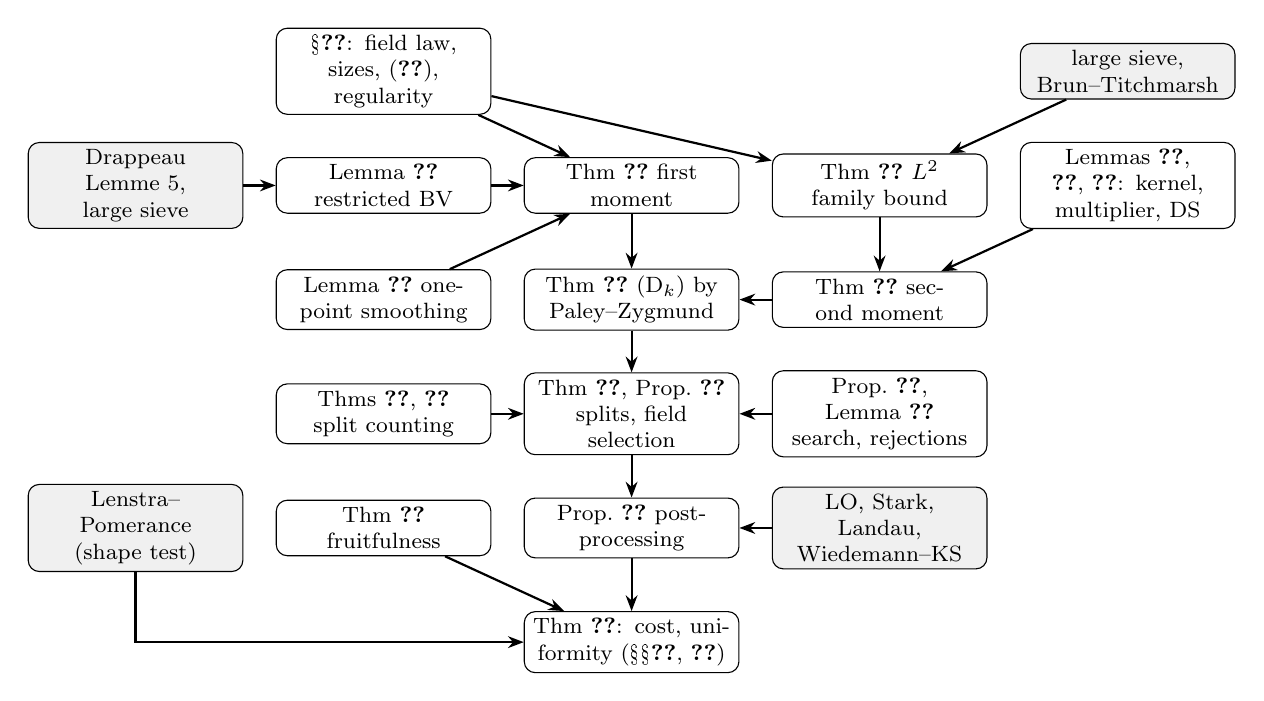
\begin{tikzpicture}[
  box/.style={draw,rounded corners,align=center,font=\footnotesize,inner sep=2.5pt,minimum height=7mm,text width=2.55cm},
  pub/.style={box,fill=gray!12},
  arr/.style={-{Stealth[length=2mm]},thick},
  x=3.15cm,y=1.45cm]
\node[box] (SETUP) at (1,1) {\S\ref{sec:algorithm}: field law, sizes, \eqref{eq:forced}, regularity};
\node[pub] (LS) at (4,1) {large sieve, Brun--Titchmarsh};
\node[pub] (LV) at (0,0) {Drappeau Lemme~5, large sieve};
\node[box] (L85) at (1,0) {Lemma~\ref{lem:85} restricted BV};
\node[box] (FM) at (2,0) {Thm~\ref{thm:FM} first moment};
\node[box] (L2) at (3,0) {Thm~\ref{thm:L2} $L^2$ family bound};
\node[box] (KW) at (4,0) {Lemmas \ref{lem:kern}, \ref{lem:W}, \ref{lem:DS}: kernel, multiplier, DS};
\node[box] (SM1) at (1,-1) {Lemma~\ref{lem:smooth1} one-point smoothing};
\node[box] (PZ) at (2,-1) {Thm~\ref{thm:Dk} $(\mathrm D_k)$ by Paley--Zygmund};
\node[box] (LD) at (3,-1) {Thm~\ref{thm:LD} second moment};
\node[box] (S) at (1,-2) {Thms \ref{thm:S}, \ref{thm:Sprime} split counting};
\node[box] (K) at (2,-2) {Thm~\ref{thm:K}, Prop.~\ref{prop:select} splits, field selection};
\node[box] (BS) at (3,-2) {Prop.~\ref{prop:BS}, Lemma~\ref{lem:reject} search, rejections};
\node[box] (DD) at (1,-3) {Thm~\ref{thm:DD} fruitfulness};
\node[box] (LV6) at (2,-3) {Prop.~\ref{prop:lv6} post-processing};
\node[pub] (NT) at (3,-3) {LO, Stark, Landau, Wiedemann--KS};
\node[pub] (LP) at (0,-3) {Lenstra--Pomerance (shape test)};
\node[box] (MAIN) at (2,-4) {Thm~\ref{thm:main}: cost, uniformity (\S\S\ref{sec:cost}, \ref{sec:uniform})};
\draw[arr] (LV)--(L85); \draw[arr] (L85)--(FM); \draw[arr] (SM1)--(FM); \draw[arr] (SETUP)--(FM);
\draw[arr] (SETUP)--(L2); \draw[arr] (LS)--(L2); \draw[arr] (L2)--(LD); \draw[arr] (KW)--(LD);
\draw[arr] (FM)--(PZ); \draw[arr] (LD)--(PZ); \draw[arr] (PZ)--(K); \draw[arr] (S)--(K); \draw[arr] (BS)--(K);
\draw[arr] (K)--(LV6); \draw[arr] (NT)--(LV6); \draw[arr] (LV6)--(MAIN); \draw[arr] (DD)--(MAIN);
\draw[arr] (LP)|-(MAIN);
\end{tikzpicture}
\caption{Dependencies. Shaded boxes are published results, used only through their statements. Drappeau's Lemme~5 is
published, but its proof refers to computations in Harper's unpublished preprint (Appendix~\ref{app:85}).}
\label{fig:deps}
\end{figure}

\begin{remark}[two interfaces that need care]\label{rem:interfaces}
\begin{enumerate}[label=(\alph*)]
\item \emph{Order of operations.} The moment bounds are proved under the raw product law $\cA$. Rejection
  of bad fields is then accounted for at the level of the bounded quantity $\delta_A\in[0,1]$, as
  $\Ex[\delta_A1_{\cR^c}]\ge\gamma-\Prob(\cR)$, and only after that is the field-selection rule applied. Conditioning on
  acceptance before the moment estimates would destroy the product structure that the second moment
  uses.
\item \emph{Computable $S$.} The algorithm cannot compute $\Psi$, so $S$ is an explicit function of $N$
  and $\Ex N_\ell$ need not be $\ge1$. The Paley--Zygmund form $\gamma\ge(\Ex N)^2/(\Ex N(N-1)+\Ex N)$ needs
  neither $\Ex N\ge1$ nor a polylogarithmic lower bound on $\gamma$. Indeed $S^2\rr\rF$ is $L^{o(1)}$ but,
  by de Bruijn's second-order term, smaller than every negative power of $\log N$. So only
  $\gamma\ge L^{-o(1)}$ holds, and that suffices because $k$ is fixed.
\end{enumerate}
\end{remark}

%======================================================================
\section{Split counting}\label{sec:split}
%======================================================================

In this section $N$ is odd and $h_2:=2^{\omega(N)}=[(\Z/N)^\times:Q_N]$. For a set $\cS$ of integers coprime to $N$, let $E_\cS$
be the event that $u\equiv Rv\pmod N$ for some $u,v\in\cS$, where $R$ is uniform on $Q_N$.

\begin{theorem}[split counting; ratio form of the Dixon--Pomerance lemma]\label{thm:S}
Let $Y'\ge2$ with $2Y'^2<N$, and let $\cS\subset[Y'/2,Y']\cap\Z$ consist of integers coprime to $N$. Then
\[
\Prob[E_\cS]\ \ge\ \frac{|\cS|^4}{2h_2\varphi(N)Y'^2(1+\log Y')}.
\]
Moreover, if $(u,v)\in\cS^2$ satisfies $u\equiv Rv$, then $(u,v)$ is an integer multiple of a shortest nonzero
vector $(u_0,v_0)$ of $\Lambda_R=\{(x,y)\in\Z^2:x\equiv Ry\pmod N\}$.
\end{theorem}

\begin{proof}
Put $n(R):=\#\{(u,v)\in\cS^2:u\equiv Rv\}$ for $R\in Q_N$.

\emph{First moment.} Let $\widehat G$ be the group of characters of $(\Z/N)^\times$ trivial on $Q_N$, so $|\widehat G|=h_2$, every
$\chi\in\widehat G$ is real, and $1[x\in Q_N]=h_2^{-1}\sum_{\chi\in\widehat G}\chi(x)$. Then
\[
\sum_{R\in Q_N}n(R)=\#\{(u,v)\in\cS^2:uv^{-1}\in Q_N\}=h_2^{-1}\sum_{\chi\in\widehat G}\Bigl(\sum_{u\in\cS}\chi(u)\Bigr)^2\ \ge\ |\cS|^2/h_2,
\]
by keeping only the trivial character.

\emph{Second moment.} If $u\equiv Rv$ and $u'\equiv Rv'$ then $uv'\equiv u'v\pmod N$ and $|uv'-u'v|<Y'^2<N$, so $uv'=u'v$:
the two vectors are proportional. Write $g=\gcd(u,v)$ and $(u,v)=g(u_1,v_1)$. The vectors of $\cS^2$
proportional to $(u,v)$ are of the form $j(u_1,v_1)$ with $ju_1\in[Y'/2,Y']$, and there are at most $Y'/(2u_1)+1\le2g$ of
them. Hence
\[
\sum_{R}n(R)^2\le\sum_{(u,v)\in\cS^2}2\gcd(u,v)\le2\sum_{g\ge1}g\lfloor Y'/g\rfloor^2\le2Y'^2(1+\log Y').
\]
\emph{Cauchy--Schwarz.} $\#\{R:n(R)>0\}\ge(\sum n)^2/\sum n^2$. Dividing by $|Q_N|=\varphi(N)/h_2$ gives the bound.

\emph{Shortest vector.} $\Lambda_R$ has determinant $N$. Let $(u,v)\in\cS^2\cap\Lambda_R$ and let $(u_0,v_0)$ be a shortest vector. Both have
Euclidean norm at most $\sqrt2Y'$, so $|uv_0-u_0v|\le2Y'^2<N$ by Cauchy--Schwarz. The determinant is a multiple of $N$, hence $0$,
and the vectors are proportional. A shortest vector is primitive in $\Lambda_R$, so $(u,v)\in\Z(u_0,v_0)$.
\end{proof}

\begin{theorem}[$k$-products]\label{thm:Sprime}
Let $\cD$ be a set of primes in a dyadic interval, all coprime to $N$, with $n:=|\cD|\ge4k^2$. Let $\cS$ be a set of
products of exactly $k$ distinct primes of $\cD$, contained in a window $[Y'/2,Y']$ with $2Y'^2<N$, and
with $|\cS|\ge\binom nk/(2k)$. Then
\[
\Prob[E_\cS]\ \ge\ \frac{|\cS|^2}{c_kh_2\varphi(N)},\qquad c_k:=8k^2\binom{2k}{k}.
\]
\end{theorem}

\begin{proof}
As before $\sum_Rn(R)\ge|\cS|^2/h_2$ and $\sum_Rn(R)^2\le\sum_{(u,v)\in\cS^2}\#\{\text{partners of }(u,v)\}$, where the partners are the elements of
$\cS^2$ proportional to $(u,v)$. Classify $(u,v)$ by the number $i$ of primes that $u$ and $v$ share. Then
$(u,v)=(ju_1,jv_1)$ with $j$ the product of the $i$ shared primes. There are at most $\binom ni\binom n{k-i}^2$ such pairs,
and each has at most $\binom ni$ partners $j'(u_1,v_1)$. Now
\[
\binom ni\binom n{k-i}=\binom ki\binom nk\prod_{t<i}\frac{n-t}{n-k+i-t}\le\binom ki\binom nk\Bigl(1+\frac k{n-k}\Bigr)^k\le\sqrt2\binom ki\binom nk,
\]
since $k^2/(n-k)\le1/3$ for $n\ge4k^2$ and $e^{1/3}<\sqrt2$. So the $i$-th class contributes at most
$2\binom ki^2\binom nk^2\le8k^2\binom ki^2|\cS|^2$. Summing, with $\sum_i\binom ki^2=\binom{2k}k$, gives $\sum n(R)^2\le c_k|\cS|^2$, and
Cauchy--Schwarz finishes the proof as before.
\end{proof}

\begin{remark}
No independence, no distribution of the primes and no character sum is used. The
square-class condition is absorbed by positivity, which is Dixon's coset pigeonhole written with
characters. The factor $2^{\omega(N)}$ is harmless after trial division (Lemma~\ref{lem:omega}).
\end{remark}

\begin{lemma}[small factors]\label{lem:omega}
If $N$ has no prime factor $\le B$, then $\omega(N)\le\log N/\log B$ and $2^{\omega(N)}=L^{o(1)}$.
\end{lemma}

\begin{proof}
$\omega(N)\log B\le\log N$, and $\log N/\log B\asymp(\log N/\log\log N)^{1/2}=o(\cL)$.
\end{proof}

%======================================================================
\section{Fruitfulness: Dixon descent}\label{sec:DD}
%======================================================================

\begin{theorem}[Dixon descent; Rabin/Dixon fibre symmetry]\label{thm:DD}
Let $N$ be odd with $\omega(N)\ge2$. Let $r_1,r_2,\dots$ be independent and uniform on $[1,N-1]$, let $R_i:=r_i^2\bmod N$, and let
$\xi$ be further randomness independent of $(r_i)$. Let $\cF:=\sigma((R_i)_i,\xi)$. Let $\cE\in\cF$ be an event on which
an $\cF$-measurable nonempty finite set $\sS$ of indices with every $R_i$ ($i\in\sS$) a unit, and an $\cF$-measurable
$\sY\in(\Z/N)^\times$, are given, with
$\sX^2\equiv\sY^2\pmod N$ where $\sX:=\prod_{i\in\sS}r_i$. Then, conditional on $\cF$, on $\cE$ the ratio $\sX/\sY$ is uniform on $\bmu$, and
\[
\Prob\bigl[1<\gcd(\sX-\sY,N)<N\,\big|\,\cF\bigr]=1-2^{1-\omega(N)}\ge\tfrac12\qquad\text{on }\cE.
\]
\end{theorem}

\begin{proof}
For every unit square $R$ fix a root $\rho(R)$. Conditional on $R_i$ (a unit), $r_i=\epsilon_i\rho(R_i)$ with $\epsilon_i$ uniform on
$\bmu$, because each unit square has exactly $|\bmu|$ roots and $r_i$ is uniform. These $\epsilon_i$ are independent of
each other and of $\xi$. So, conditional on $\cF$, they are i.i.d.\ uniform on $\bmu$. On $\cE$,
$\sX/\sY=\prod_{i\in\sS}\epsilon_i\cdot\prod_{i\in\sS}\rho(R_i)\sY^{-1}$, where the second factor is $\cF$-measurable and lies in
$\bmu$ (both $\sX/\sY$ and the first factor do). A product of independent uniform elements of a finite group over a nonempty
index set is uniform, so $\sX/\sY$ is uniform on $\bmu$. Finally, for $\zeta\in\bmu$ and the
factorisation $N=\prod p_j^{e_j}$ we have $\zeta\equiv\pm1\pmod{p_j^{e_j}}$ for each $j$, and $\zeta-1$ is a unit modulo
$p_j^{e_j}$ when $\zeta\equiv-1$ there ($N$ is odd). Hence $\gcd(\sX-\sY,N)=\gcd(\zeta-1,N)=\prod_{\zeta\equiv1\,(p_j^{e_j})}p_j^{e_j}$ with
$\zeta=\sX/\sY$, which is proper unless $\zeta=\pm1$. These are $2$ of the $2^{\omega(N)}$ elements.
\end{proof}

\begin{remark}[transcript invariance in Algorithm~\ref{alg:split}]\label{rem:T}
We check that SPLIT satisfies the hypothesis of Theorem~\ref{thm:DD} in each round. Every
quantity computed before $\sX_\sS$ is a function of the squares $R_i$ and of coins independent of the roots. This covers:
\begin{itemize}
\item the field $(g,w,c)$ and its checks;
\item the Gauss reduction of $\Lambda_{R_i}$ (with a fixed tie rule) and the Lenstra--Pomerance factorisation of $|u_0|,|v_0|$,
  whose coins are fresh;
\item the shape decision, and the special-$q$ searches with their cache, which depend on $(A,\ell)$ only;
\item the gcd checks (the unit status of $r_i$ is that of $R_i$);
\item all columns, characters, kernel vectors, the Hensel prime, square-root branches, the choice among three dependencies, and
  $\sY_\sS$ (Section~\ref{sec:lv6}).
\end{itemize}
The roots enter only through $\sX_\sS$. After a trivial gcd, all rows are discarded and the next round
uses fresh roots. For that round we apply Theorem~\ref{thm:DD} with $\xi$ containing everything from earlier rounds, including the
old roots, which are independent of the new ones. Field retention biases the law of the field and of
the accepted $R_i$, but not of the fibre signs $\epsilon_i$.

Two cautions. (i) Exactness needs $r$ uniform on all of $[1,N-1]$. Drawing from $[2,N-2]$, for instance, breaks it: at $N=15$,
$R=1$, the remaining roots $4,11$ both give proper factors. (ii) Accepted roots are \emph{not} uniform on $(\Z/N)^\times$,
because acceptance filters $R$. What holds, and what is used, is uniformity on the fibre $r_i\bmu$ given $\cF$.
\end{remark}

%======================================================================
\section{Bounded-\texorpdfstring{$k$}{k} splits and field selection}\label{sec:K}
%======================================================================

From now on $N$ is the input of SPLIT: odd, with no prime factor $\le B$ and not a prime power, and $N\ge N_0$.

\begin{lemma}[reverse Markov]\label{lem:revmarkov}
If $Z\in[0,1]$ and $\Ex Z\ge\beta$, then $\Prob[Z\ge\beta/2]\ge\beta/2$.
\end{lemma}

\begin{proof}
$\beta\le\Ex Z\le\beta/2+\Prob[Z\ge\beta/2]$.
\end{proof}

\begin{theorem}[complete descents in one field]\label{thm:K}
Let $A$ be a field for which $\mathrm{SAMPLE\_FIELD}$ returns $A$ (no rejection and no factor exit), and suppose
$|\cD_A|\ge4k^2$. Then one call of $\mathrm{DESCEND\_ONCE}(A)$ returns a row or makes a factor exit with probability at
least
\[
c_k'\Bigl(\frac{\delta_A}{\log N}\Bigr)^{2k}2^{-\omega(N)},
\]
with $c_k'>0$ depending only on $k$.
\end{theorem}

\begin{proof}
The products of $k$ distinct primes of $\cD_A\subset J$ lie in $(Y^k,(2Y)^k]\subset(X2^{-2k},X]$. By pigeonhole one of the $2k$
dyadic windows $[Y'/2,Y']$ with $Y'=X2^{-i}$, $0\le i<2k$, contains a set $\cS$ of at least $\binom{|\cD_A|}k/(2k)$ of them, and
$2Y'^2\le2X^2<N$ (Lemma~\ref{lem:sizes}(e)).
Every $\ell\in\cD_A$ satisfies $\ell\nmid N$, by definition of $N_\ell$. Let $E$ be the event that $r$ is a unit and $R\equiv u/v$
with $u,v\in\cS$. Given that $r$ is a unit, $R$ is uniform on $Q_N$, so Theorem~\ref{thm:Sprime} gives
\[
\Prob_r[E]\ge\frac{\varphi(N)}{N}\cdot\frac{|\cS|^2}{c_kh_2\varphi(N)}=\frac{|\cS|^2}{c_kh_2N}.
\]
Now $|\cS|\ge(|\cD_A|/k)^k/(2k)$ and $|\cD_A|=\delta_A\pi_J\ge\delta_AY/(2\log Y)$, while
$Y^{2k}\ge X^2/16^k\ge N/(4\cdot16^k)$ and $2k\log Y\le\log N$. This gives the displayed lower bound for $\Prob_r[E]$.

On $E$, Theorem~\ref{thm:S} shows $(u,v)=j(u_0,v_0)$. Unless a gcd check exits, $|u_0|$ and $|v_0|$ divide $u$ and $v$, so
each is a product of at most $k$ distinct primes of $\cD_A$. (This is why the rule says \emph{at most} $k$: the
condition is closed under taking divisors, whereas ``exactly $k$'' is not.) So the shape test passes. For each such
$\ell$ we have $N_\ell(A)\ge1$, and by Proposition~\ref{prop:BS} $\mathrm{SQ\_SEARCH}(A,\ell)$ returns an atom unless a gcd check
exits first. Hence the call returns a row or exits with a factor.
\end{proof}

\paragraph{Trials and costs.} A \emph{trial} is one call of SAMPLE\_FIELD followed, if a field is returned, by one call
of DESCEND\_ONCE. Its outcome is a factor exit, a row, or neither. Let $p_F$ and $b$ be the probabilities of the first two
outcomes and $p:=p_F+b$. For a field $A$ let $\varsigma_A$ be the probability that DESCEND\_ONCE$(A)$ returns a row ($\varsigma_A:=0$
for rejected fields and for fields on which SAMPLE\_FIELD exits). Let $C_{\rm trial}$ be a uniform upper bound for the
expected cost of one trial and of one call of DESCEND\_ONCE, conditional on everything before it.
Let $\mathrm T_{\rm post}$ be a uniform bound for the expected cost of POSTPROCESS. Let $\cR$ be the set of fields rejected in steps~2--4 of
SAMPLE\_FIELD, regardless of exits.

\begin{proposition}[field selection with factor exits]\label{prop:select}
\begin{enumerate}[label=(\roman*)]
\item If $\gamma\ge L^{-o(1)}$ and $\Prob_\cA(\cR)\le\gamma/2$, then $p\ge L^{-o(1)}$.
\item The expected running time of $\mathrm{SPLIT}(N)$ is at most $3(M_{\rm rows}C_{\rm trial}+\mathrm T_{\rm post})/p$.
\end{enumerate}
\end{proposition}

\begin{proof}
(i) Since $0\le\delta_A\le1$, $\Ex[\delta_A1_{\cR^c}]\ge\gamma-\Prob(\cR)\ge\gamma/2$. By Lemma~\ref{lem:revmarkov}, the set
$\cG^*:=\{A\notin\cR:\delta_A\ge\gamma/4\}$ has probability at least $\gamma/4$. For $A\in\cG^*$, either SAMPLE\_FIELD exits
with a factor, or it returns $A$. In the latter case $|\cD_A|\ge\gamma\pi_J/4\ge4k^2$ for large $N$ (as
$\pi_J=N^{2\nu+o(1)}$), and Theorem~\ref{thm:K} applies. Hence
$p\ge(\gamma/4)c_k'(\gamma/(4\log N))^{2k}2^{-\omega(N)}=L^{-o(1)}$, by Lemma~\ref{lem:omega} and because $k$ is fixed.

(ii) Trials are i.i.d., so the number of trials until the outcome is a factor or a row is geometric with
mean $1/p$. By Wald's identity the expected cost of selection is at most $C_{\rm trial}/p$. On a factor exit we are done.
Otherwise the outcome is a row, and the kept field $A^*$ has law $\Prob[A^*\in dA]=\varsigma_A\Prob_\cA(dA)/b$. Given $A^*=A$, a
round collects $M_{\rm rows}$ rows with an expected $M_{\rm rows}/\varsigma_A$ calls (or ends earlier with a factor), at expected cost at most
$M_{\rm rows}C_{\rm trial}/\varsigma_A+\mathrm T_{\rm post}$. By Theorem~\ref{thm:DD} and Remark~\ref{rem:T}, each round that reaches its final gcd succeeds with
conditional probability at least $1/2$, whatever happened before. So the expected cost given $A^*=A$ is at most
$2(M_{\rm rows}C_{\rm trial}/\varsigma_A+\mathrm T_{\rm post})$. Averaging over the law of $A^*$,
\[
\Ex\bigl[1/\varsigma_{A^*}\bigr]=\int\frac1{\varsigma_A}\frac{\varsigma_A}{b}\,\Prob_\cA(dA)=\frac{\Prob(\varsigma_A>0)}{b}\le\frac1b.
\]
The kept-field branch is reached with probability $b/p$, so its contribution is at most
$(b/p)\cdot2(M_{\rm rows}C_{\rm trial}/b+\mathrm T_{\rm post})\le2(M_{\rm rows}C_{\rm trial}+\mathrm T_{\rm post})/p$. Factor exits during collection only shorten the run.
\end{proof}

\begin{remark}
No lower bound on $\varsigma_A$ for the kept field is used: the harmonic-mean identity makes the cost
depend only on $b$. Nor do we claim that the law of the non-terminating fields retains $\gamma/2$. Factor exits are
absorbed as successful outcomes, which repairs a gap in an earlier draft of the argument.
\end{remark}

%======================================================================
\section{The first moment}\label{sec:FM}
%======================================================================

\subsection{One-point smoothing}
The coefficient vector $c$ enters $F_A(P)$ only through $\langle c,v(P)\rangle$. The next lemma replaces Lee and
Venkatesan's Lemmas~5.13, 5.18 and~5.20 \cite{lv2018} by a short self-contained argument.

\begin{lemma}[one-point smoothing]\label{lem:smooth1}
Let $P=(a,b)$ with $\gcd(a,b)=1$ and $ab\ne0$, put $V'=\max(|a|,|b|)$ and $l_i=|a|^{d-1-i}|b|^i$, and let $H\ge3dV'$. For $c$ uniform on
$C_H$ there is a probability measure $\vartheta$ on $\Z$ such that:
\begin{enumerate}[label=(\alph*)]
\item $\|\mathrm{Law}(\langle c,v(P)\rangle)-\vartheta\|_{\rm TV}\le3d^2V'/(2H+1)$;
\item $\vartheta$ is the law of $\sum_iY_i$ with $Y_i$ independent and uniform on integer intervals of lengths $(2H+1)l_i$;
\item $\vartheta(z)$ is a non-increasing function of $|z-M_0|$ for some $M_0\in\frac12\Z$ with $|M_0|\le dV'^{d-1}$;
\item $\max_z\vartheta(z)\le1/((2H+1)V'^{d-1})$.
\end{enumerate}
\end{lemma}

\begin{proof}
Write $v=v(P)$. Its entries have $\gcd(a^{d-1},b^{d-1})=1$. The vectors $u_j:=b\,e_j-a\,e_{j+1}$ ($0\le j\le d-2$)
lie in $\ker\langle\cdot,v\rangle$. The maximal minor of the matrix with rows $u_j$ that omits column $i$ equals
$\pm a^{d-1-i}b^i$, so the gcd of the maximal minors is $1$, and the $u_j$ are a basis of the lattice
$K:=\{x\in\Z^d:\langle x,v\rangle=0\}$. Each coordinate of a point $\sum s_ju_j$ with $s\in[0,1)^{d-1}$ has absolute value at most
$|a|+|b|\le2V'$.

\emph{Representations.} Let $m\in\Z$ with $|m|\le\|v\|_2$. Since $\gcd$ of the entries is $1$, the integer solutions of
$\langle x,v\rangle=m$ form a coset $x_0+K$. The real point $p_m:=mv/\|v\|_2^2$ lies on the same affine hyperplane and
has $\|p_m\|_\infty\le|m|/\|v\|_2\le1$. Writing $p_m-x_0=\sum s_ju_j$ and $x:=x_0+\sum\lfloor s_j\rfloor u_j$, we get
$\langle x,v\rangle=m$ and $\|x\|_\infty\le1+2V'$.

\emph{Smoothing.} Since $l_i\le V'^{d-1}\le\|v\|_2$, for each $i$ we may fix a set $S_i$ of $l_i$ vectors with
$\|x\|_\infty\le3V'$ on which $\langle\cdot,v\rangle$ is a bijection onto $\{0,\dots,l_i-1\}$. Let $x^{(i)}$ be uniform on $S_i$,
independent of each other and of $c$, and put $c':=c+\sum_ix^{(i)}$. Then
$\langle c',v\rangle=\sum_iY_i$ with $Y_i:=c_iv_i+\langle x^{(i)},v\rangle$. Here $c_iv_i=\pm c_il_i$ with $\pm c_i$ uniform on
$[-H,H]$, so $Y_i$ is uniform on an integer interval of length $(2H+1)l_i$. The $Y_i$ are independent. Let $\vartheta$ be the
law of $\sum Y_i$. For a fixed shift $y$, the uniform measures on $C_H$ and $C_H+y$ differ in total variation by
at most $\|y\|_1/(2H+1)$. Hence $\|\mathrm{Law}(c)-\mathrm{Law}(c')\|_{\rm TV}\le d\cdot3dV'/(2H+1)$, and (a) follows by
applying the map $\langle\cdot,v\rangle$.

(c) A uniform distribution on an integer interval is a log-concave sequence, symmetric about the midpoint of the
interval. Convolutions of log-concave sequences without internal zeros are log-concave (see e.g.\
\cite{stanley1989}), and a log-concave sequence is unimodal. A symmetric unimodal sequence is
non-increasing in the distance to its centre. The centre of $Y_i$ is $(l_i-1)/2$ or its negative, so $|M_0|\le\sum l_i/2\le dV'^{d-1}$.
(d) A convolution of probability measures has maximum at most the maximum of any factor. Take the factor with
$l_i=V'^{d-1}$.
\end{proof}

By (c), $\vartheta$ has a layer-cake decomposition
\begin{equation}\label{eq:layer}
\vartheta=\sum_mW_m\,\mathrm{Unif}\bigl([M_0-y_m,M_0+y_m]\cap\Z\bigr),\qquad W_m\ge0,\ \ \sum_mW_m=1,
\end{equation}
because every level set $\{z:\vartheta(z)\ge s\}$ is an integer interval symmetric about $M_0$.

\subsection{Good moduli}
Put $\varpi:=L$ and
\[
\cX:=\bigl\{\XF\varpi^{-2}(3/2)^i:i\ge0\bigr\}\cap\bigl[\XF\varpi^{-2},\,16d\XF\bigr],\qquad|\cX|=O(\cL).
\]
The grid $\cX$ does not depend on $\ell$, $P$, $g$, $w$, or any residue.

\begin{definition}\label{def:good}
A positive integer $t$ is \emph{good} if, for every $x\in\cX$ and every $r$ with $(r,t)=1$,
$|\Psi(x;t,r)-\Psi_t(x)/\varphi(t)|\le\Psi_t(x)/(2\varphi(t))$. Otherwise $t$ is \emph{bad}.
\end{definition}

\begin{lemma}[algebraic smoothness at a good modulus]\label{lem:goodmod}
Let $N\ge N_0$. Let $\ell\in J$, $P=(a,b)\in\cP_\ell$, $g\in\cG$ and $w$ be such that $t:=|G(P)|\in[MV_\ell/32,2MV_\ell]$, $t$ is good,
and $r_0:=\hat F_{g,w}(P)\bmod t$ satisfies $(r_0,t)=1$. Then
\[
\Prob_c\bigl[F_A(P)\in\cS_B\bigr]\ \ge\ \rF/(\log N)^{C}.
\]
\end{lemma}

\begin{proof}
Write $V=V_\ell$, $V'=\max(|a|,b)\in(V/2,V]$, $\hat F=\hat F_{g,w}(P)$ and $G=G(P)$. Since $F_A(P)=\hat F+G\langle c,v(P)\rangle$ and
$H\ge3dV'$, Lemma~\ref{lem:smooth1} gives
$\Prob_c[F_A(P)\in\cS_B]\ge\Prob_{Z\sim\vartheta}[\hat F+GZ\in\cS_B]-3d^2V/(2H+1)$. Use \eqref{eq:layer} and put
$Y_\varpi:=(2H+1)V'^{d-1}/\varpi$.

\emph{Small layers.} The layers with $y_m<Y_\varpi$ are supported in $|z-M_0|<Y_\varpi$, a set of $\vartheta$-mass at most
$(2Y_\varpi+1)/((2H+1)V'^{d-1})\le3/\varpi$ by Lemma~\ref{lem:smooth1}(d).

\emph{One large layer.} Fix $m$ with $y:=y_m\ge Y_\varpi$ and put $y':=\lfloor y/2\rfloor$. Since $|M_0|\le dV'^{d-1}\le Y_\varpi/2$, the
layer's interval contains $[0,y']$ and $[-y',0]$. Consider $z\in[0,y']$. The values $\hat F+Gz$ are all integers $\equiv
r_0\pmod t$ between $\hat F$ and $\hat F+Gy'$. If $G>0$ they include every $n\equiv r_0$ with $|\hat F|<n\le ty'-|\hat F|$. If $G<0$
they include every $n\equiv r_0$ with $-(ty'-|\hat F|)\le n<-|\hat F|$, that is, every $-n\equiv-r_0$ in the same range of $|n|$. So,
with $r'=\pm r_0$ (a reduced residue),
\[
\#\{0\le z\le y':\hat F+Gz\in\cS_B\}\ \ge\ \Psi(x_1;t,r')-\Psi(|\hat F|;t,r')
\]
for any $x_1\le ty'-|\hat F|$. By Lemma~\ref{lem:valuesizes}, $|\hat F|\le C_dMHV^dN^{-\eta_0/2}$, while
$ty'\ge(MV/32)(Y_\varpi/2-1)\ge c_dMHV^d/\varpi$. So $|\hat F|\le ty'/4$, and also $ty'/4\ge\XF\varpi^{-2}$ and
$ty'/2\le2MV\cdot d(H+1)V^{d-1}\le16d\XF$. Consecutive points of $\cX$ differ by the factor $3/2<2$, so we may take
$x_1\in\cX\cap(ty'/4,ty'/2]$. Since $t$ is good, and by Fact~\ref{fact:Ten} (here $\omega(t)\le\log N$, so its error
term is $o(1)$),
\[
\Psi(x_1;t,r')\ge\frac{\Psi_t(x_1)}{2\varphi(t)}\ge\frac{\Psi(x_1)}{3t}\ge\frac{y'}{12}\varrho(ty'/4)\ge\frac{y'\rF}{(\log N)^{C}},
\]
using Lemma~\ref{lem:local}(i),(ii): $ty'/4$ and $\XF$ differ by a factor $\le\varpi^2\le B^{C}$. Trivially
$\Psi(|\hat F|;t,r')\le|\hat F|/t+1$. The same bound holds for $z\in[-y',0]$. Dividing by the $2y+1$ points of the layer,
the proportion of smooth values in the layer is at least
\[
\frac{\rF}{3(\log N)^C}-\frac{|\hat F|/t+1}{y}\ \ge\ \frac{\rF}{3(\log N)^C}-C\varpi N^{-\eta_0/2}.
\]
\emph{Conclusion.} $\Prob_c\ge(1-3/\varpi)\bigl(\rF/(3(\log N)^C)-C\varpi N^{-\eta_0/2}\bigr)-3d^2V/(2H+1)$. Here $\rF=L^{-O(1)}$,
$\varpi=L$ and $V/H\le N^{-\nu-\eta_0}$, so the error terms are negligible.
\end{proof}

\subsection{Bad moduli are rare}
The next lemma is a restricted Bombieri--Vinogradov estimate for moduli of the form $\ell\cdot(\text{smooth})$.
It is the analogue of Lee--Venkatesan's Lemma~8.5 \cite{lv2018} for these moduli. Its proof, in Appendix~\ref{app:85}, does not use
that lemma; it rests on the exact identity of Lemma~\ref{lem:E2}, the large sieve, and Drappeau's Lemme~5.

\begin{lemma}[restricted BV for the moduli $\ell s$; ``Lemma~8.5$'$'']\label{lem:85}
Fix $\xi>0$ and $q_0$ with $2\nu<q_0<\xi/2$. Let $x=N^{\xi+o(1)}$ and $Q=N^{q_0+o(1)}$, and let
\[
\cT_Q:=\{t=\ell s\in(Q/2,Q]:\ \ell\in J,\ s\ge1,\ \Pp(s)\le B\}.
\]
Then, uniformly in such $x,Q$,
\[
\sum_{t\in\cT_Q}\ \max_{(r,t)=1}\Bigl|\Psi(x;t,r)-\frac{\Psi_t(x)}{\varphi(t)}\Bigr|\ \le\ \varepsilon_N\,\Psi(x)\,\frac{\#\cT_Q}{Q},
\]
where $\varepsilon_N=C\exp\bigl(-c_0(\log N)^{1/2}(\log\log N)^{-5/2}\bigr)$ for some fixed $C,c_0>0$. In particular
$\varepsilon_N(\log N)^{A}\to0$ for every fixed $A$.
\end{lemma}

\begin{corollary}\label{cor:bad}
In the setting of Lemma~\ref{lem:85} with $x$ ranging over $\cX$, the number of bad $t\in\cT_Q$ is at most $3|\cX|\varepsilon_N\#\cT_Q$.
\end{corollary}

\begin{proof}
If $t\in\cT_Q$ is bad, there are $x\in\cX$ and $(r,t)=1$ with
$|\Psi(x;t,r)-\Psi_t(x)/\varphi(t)|>\Psi_t(x)/(2\varphi(t))\ge\Psi(x)/(3t)\ge\Psi(x)/(3Q)$, by Fact~\ref{fact:Ten}. Sum
Lemma~\ref{lem:85} over $x\in\cX$ and apply Markov's inequality.
\end{proof}

\subsection{Rational fibres}

\begin{lemma}[fibres]\label{lem:fibres}
Fix $\ell\in J$ and $P=(a,b)\in\cP_\ell$, and put $\cG_P(n):=\{g\in\cG:G_g(P)=\ell n\}$.
\begin{enumerate}[label=(\roman*)]
\item The $g\in\Z^2$ with $G_g(P)=\ell n$ form a line $g^*+\Z(a,b)$, and $|\cG_P(n)|\le\sqrt2M/V_\ell+1\le2M/V_\ell$ for every $n$.
\item There is a set $I_P$ of consecutive integers $n$, of length at least $MV_\ell/(16\ell)-1$, on which $\ell n$ has constant sign,
  $MV_\ell/32\le\ell|n|\le2MV_\ell$, and $|\cG_P(n)|\ge M/(CV_\ell\log\log N)$.
\end{enumerate}
\end{lemma}

\begin{proof}
Write $V=V_\ell$. (i) $G_g(P)=g_1a-g_0b$ is constant along the direction $(a,b)$, which is primitive with
$|(a,b)|\ge b>V/2$, and the square $[M/2,M]^2$ has diameter $M/\sqrt2$.

(ii) Let $(g_0,g_1)$ be uniform on the real square $[M/2,M]^2$. Then $G=ag_1-bg_0$ is a sum of independent uniform
variables on intervals of lengths $\alpha\le\beta$ with $\beta=V'M/2$, $V'=\max(|a|,b)$. Its density is at least $1/(2\beta)$ on an
interval of length $\beta$. The density at $s$ equals (length of the chord $\{G=s\}$)$/(|(a,b)|M^2/4)$, so on that interval the
chord has length at least $(1/(V'M))\cdot V'\cdot M^2/4=M/4$. Removing $(-MV/32,MV/32)$ from an interval of length $\ge MV/4$
leaves a subinterval of length $\ge MV/16$ of constant sign. Let $I_P$ be the integers $n$ with $\ell n$ in it. For $n\in I_P$
the fibre line meets the closed square in at least $\lfloor(M/4)/|(a,b)|\rfloor\ge M/(8V)$ consecutive lattice points
$g^*+j(a,b)$.

\emph{Coprimality.} Fix $e\ge1$. Choose $x,y$ with $xa+yb=1$. If $e\mid\gcd(g_0,g_1)$ then $e\mid G=\ell n$. Conversely, if $e\mid\ell n$,
the $j$ with $e\mid g^*+j(a,b)$ are exactly those with $j\equiv-(xg_0^*+yg_1^*)\pmod e$: the matrix
$\bigl(\begin{smallmatrix}x&y\\-b&a\end{smallmatrix}\bigr)$ has determinant $1$ and maps $g$ to $(xg_0+yg_1,G)$. By M\"obius
inversion over $e\mid\ell|n|$, the number of coprime points among $J_0\ge M/(8V)$ consecutive ones is at least
$J_0\varphi(\ell|n|)/(\ell|n|)-2^{\omega(\ell|n|)}$. Finally $\varphi(m)/m\gg1/\log\log m$, and $2^{\omega(m)}=N^{o(1)}$ is small
compared with $M/V\ge N^{\eta_0/2}$ (Lemma~\ref{lem:sizes}(c)).
\end{proof}

\subsection{The first moment}

\begin{theorem}[first moment]\label{thm:FM}
For $N\ge N_0$,
\[
\Ex_{\ell\in J}\Ex_{A\sim\cA}N_\ell(A)\ \ge\ \frac{S^2\rr\rF}{(\log N)^{C}}.
\]
\end{theorem}

\begin{proof}
At most $O(1)$ primes of $J$ divide $N$, and we drop them. For $\ell\nmid N$,
\[
\Ex_AN_\ell(A)\ \ge\ \frac1{|\cG|}\sum_{P\in\cP_\ell}\ \sum_{\substack{n\in I_P,\ n\in\cS_B\\ \ell|n|\text{ good}}}\ \sum_{g\in\cG_P(n)}\Ex_w\Prob_c\bigl[F_A(P)\in\cS_B\bigr].
\]
This is an inequality, because the filter $|G(P)|\ge MV_\ell/32$ holds on $I_P$ and the other $n$ are dropped. For these
$(\ell,P,n,g)$ and every $w$, Lemma~\ref{lem:coprime} shows that $r_0$ is reduced, so Lemma~\ref{lem:goodmod} bounds the inner
probability below by $\rF/(\log N)^C$. Hence
\[
\Ex_AN_\ell(A)\ge\frac{\rF}{(\log N)^C|\cG|}\sum_{P\in\cP_\ell}\Bigl(\sum_{n\in I_P\cap\cS_B}|\cG_P(n)|-\frac{2M}{V_\ell}\beta_\ell\Bigr),
\]
where $\beta_\ell:=\#\{n:1\le|n|\le2MV_\ell/\ell,\ n\in\cS_B,\ \ell|n|\text{ bad}\}$ depends on $\ell$ only.

\emph{Good mass.} $I_P$ is an interval of length $\lambda\ge MV_\ell/(16\ell)-1$ whose right end (in absolute value) is at most
$32\lambda$. By Lemma~\ref{lem:local}(iii),(i) it contains at least $c\lambda\rr$ smooth integers. By Lemma~\ref{lem:fibres}(ii),
$\sum_{n\in I_P\cap\cS_B}|\cG_P(n)|\ge cM^2\rr/(\ell\log\log N)$.

\emph{Bad mass.} The moduli $\ell|n|$ counted by the $\beta_\ell$ lie in $\bigcup_Q\cT_Q$ for $O(1)$ dyadic values $Q$ covering
$[M\Vm/32,2M\VM]$, all with $Q=N^{\mu+\nu+o(1)}$. Lemma~\ref{lem:85} applies with $\xi=\mu+h+d\nu$ and $q_0=\mu+\nu$, because
$q_0-2\nu=\mu-\nu\ge\eta_0$ and $\xi/2-q_0=(h-\mu+(d-2)\nu)/2\ge\eta_0/2$ by the level floor. By Corollary~\ref{cor:bad},
\[
\frac1{\pi_J}\sum_{\ell\in J}\beta_\ell\le\frac{2}{\pi_J}\sum_Q3|\cX|\varepsilon_N\#\cT_Q
\le C|\cX|\varepsilon_N\frac{M\VM}{Y}\rr(\log N)^C,
\]
since $\#\cT_Q\le\sum_{\ell\in J}\Psi(Q/\ell)\le C\pi_J(M\VM/Y)\rr$ by Lemma~\ref{lem:local}(i).

\emph{Assembly.} $\#\cP_\ell\asymp V_\ell^2/\log V_\ell$ (there are $\asymp V/\log V$ primes $b\in(V/2,V]$, and for each at least $V$ values of
$a$ coprime to $b$), $|\cG|\asymp M^2$, and $V_\ell^2/\ell\ge S^2/2$. Averaging over $\ell$, the good mass contributes at least
$cS^2\rr\rF/(\log N)^{C'}$. The bad mass contributes at most $CS^2\rr\rF|\cX|\varepsilon_N(\log N)^{C''}$, which is smaller by the factor
$|\cX|\varepsilon_N(\log N)^{O(1)}\to0$.
\end{proof}

\begin{remark}
The bound is averaged over $\ell\in J$ as well as over the field. The bad-modulus step does not give it for each
individual $\ell$, and no such statement is needed. The loss is polylogarithmic: $1/\log V$ from prime $b$, $\log\log N$ from
$\varphi(m)/m$, and the $(\log N)^{O(1)}$ of Lemma~\ref{lem:local}(ii).
\end{remark}

%======================================================================
\section{The second moment and relation supply}\label{sec:SM}
%======================================================================

Throughout this section $\ell\in J$ with $\ell\nmid N$, $V=V_\ell$, and $T=T_\ell=dHV^{d-1}$. For $P\in\cP_\ell\cap\Lambda_\ell(g)$ write
$Y_P=Y_P(g):=1$ if $|G_g(P)|\ge MV/32$ and $G_g(P)/\ell\in\cS_B$, and $Y_P:=0$ otherwise.

\subsection{Pairs in one lattice}

\begin{lemma}[pairs]\label{lem:pairs}
Let $P\ne P'$ in $\cP_\ell\cap\Lambda_\ell(g)$ and $\Delta:=\det(P,P')$. Then $\Delta\ne0$ and $\ell\mid\Delta$. Put $q:=|\Delta|/\ell$; then $q\le2S^2$. For fixed $P$ and $q$, at most $12$ points $P'\in\cP_\ell$ satisfy
$|\det(P,P')|=\ell q$.
\end{lemma}

\begin{proof}
Both points have $b,b'>0$ and are primitive, so they are not proportional and $\Delta\ne0$. They are both annihilated
modulo $\ell$ by the nonzero linear form $(x,y)\mapsto g_1x-g_0y$, so they are proportional modulo $\ell$ and $\ell\mid\Delta$. Also
$|\Delta|\le2V^2\le2\ell S^2$. For fixed $P$ and $D$, the solutions of $\det(P,P')=D$ form a line $P''+\Z P$. It meets
$[-V,V]^2$ in a segment of length at most $2\sqrt2V$, and consecutive points differ by $|P|\ge V/2$. That gives at most $6$
points for each of $D=\pm\ell q$.
\end{proof}

\begin{lemma}[kernel transfer]\label{lem:kern}
Let $d\ge3$ and let $P=(a,b)\ne P'=(a',b')$ be primitive, with $\Delta=\det(P,P')\ne0$. Put $v=v(P)$, $v'=v(P')$ and
$\Phi:\Z^d\to\Z^2$, $c\mapsto(\langle c,v\rangle,\langle c,v'\rangle)$. Let $\kappa$ be an integer with $P'\equiv\kappa P\pmod\Delta$.
\begin{enumerate}[label=(\roman*)]
\item $\Gamma:=\Phi(\Z^d)=\{(X,X')\in\Z^2:X'\equiv\kappa^{d-1}X\pmod{\Delta}\}$, of index $|\Delta|$, and $\kappa$ is a unit modulo $\Delta$.
\item $\ker\Phi=Q_{PP'}\cdot\Z[x,y]_{d-3}$ with $Q_{PP'}=(bx-ay)(b'x-a'y)$, identifying $\Z^d$ with forms of degree $d-1$.
\item If $|a|,|b|,|a'|,|b'|\le V$ and $H\ge4V^2$, then for every $z\in\Z^2$,
  $\Prob_{c\in C_H}[\Phi(c)=z]\le C_d|\Delta|/(H^2\|v\wedge v'\|)\le C_d/(H^2(bb')^{d-2})$.
\end{enumerate}
\end{lemma}

\begin{proof}
For $\gamma\in GL_2(\Z)$, $v(\gamma P)=\rho(\gamma)v(P)$ with $\rho(\gamma)\in GL_d(\Z)$ (the symmetric power). By Cauchy--Binet, the gcd of
the $2\times2$ minors of the matrix with rows $v,v'$ is unchanged. Choose $\gamma$ with $\gamma P=(1,0)$. Then $\gamma P'=(u,\pm\Delta)$ with
$\gcd(u,\Delta)=1$, and the nonzero minors of the matrix with rows $(1,0,\dots,0)$ and $v(u,\pm\Delta)$ are $\pm u^{d-1-j}\Delta^j$, $j\ge1$.
Their gcd is $|\Delta|$. Hence $\Phi(\Z^d)$ has index $|\Delta|$. In these coordinates $P'\equiv uP\pmod\Delta$, so $\kappa$ exists, is a
unit, and by homogeneity $v'\equiv\kappa^{d-1}v\pmod\Delta$. Thus $\Phi(\Z^d)$ lies in the displayed lattice, which also has
index $|\Delta|$. This proves (i).

(ii) $\langle c,v(P)\rangle=C(P)$ for the form $C=\sum c_ix^{d-1-i}y^i$. If $C(P)=C(P')=0$ then $(bx-ay)\mid C$ and $(b'x-a'y)\mid C$ over $\Q$, and the two factors are coprime
since $\Delta\ne0$. By Gauss's lemma the quotient is integral. Conversely every such multiple lies in the kernel.

(iii) The kernel $K_2$ has rank $d-2$. It is saturated, and its orthogonal complement in $\Z^d$ is the saturation of
$\Z v+\Z v'$. That lattice has determinant $\|v\wedge v'\|$ and index $|\Delta|$ in its saturation (the gcd of the minors, by (i)). A saturated
lattice and its orthogonal complement have the same determinant, so $\det K_2=\|v\wedge v'\|/|\Delta|$. The monomial
multiples of $Q_{PP'}$ form a basis of $K_2$ with entries at most $2V^2$, so a fundamental cell has $\ell^\infty$-diameter at most
$2(d-2)V^2\le dH$. A fibre $\Phi^{-1}(z)\cap C_H$ is $(c_0+K_2)\cap C_H$. The translates of the cell at its points are disjoint
and lie in the intersection of the cube $[-(d+1)H,(d+1)H]^d$ with a $(d-2)$-flat, whose $(d-2)$-volume is at most
$C_dH^{d-2}$. Hence the fibre has at most $C_dH^{d-2}|\Delta|/\|v\wedge v'\|$ points, and we divide by $(2H+1)^d$. Finally, the minor of
columns $d-2,d-1$ equals $ab^{d-2}b'^{d-1}-b^{d-1}a'b'^{d-2}=(bb')^{d-2}\Delta$, so $\|v\wedge v'\|\ge|\Delta|(bb')^{d-2}$.
\end{proof}

For candidates $b,b'>V/2$, so (iii) gives $\Prob_c[\Phi(c)=z]\le C_d/(H^2V^{2d-4})$. The kernel floor $h\ge2\nu+\eta_0$ gives
$H\ge4V^2$ for large $N$.

\subsection{The multiplier}

\begin{lemma}[residue spreading]\label{lem:W}
For $N\ge N_0$, every $1\le t\le2M\VM$ and every $r\in\Z$,
\[
\Prob_w[w\equiv r\pmod t]\le\frac{C_W}{\varphi(t)},\qquad C_W:=\frac{24}{\eta_0}.
\]
Consequently, if $(\ell,P,g)$ satisfy the hypotheses of Lemma~\ref{lem:coprime} and $\Phi_0:\Z/t\to[0,\infty)$ does not
depend on $w$, then $\Ex_w\Phi_0(\hat F_{g,w}(P)\bmod t)\le(C_W/\varphi(t))\sum_{c\in(\Z/t)^\times}\Phi_0(c)$.
\end{lemma}

\begin{proof}
If $(r,t)>1$ the probability is $0$, since every $w$ is a prime larger than $t$. Otherwise Fact~\ref{fact:BT} with $x=W$, $y=W$ gives
$\pi(2W;t,r)-\pi(W;t,r)<2W/(\varphi(t)\log(W/t))$, while $\pi(2W)-\pi(W)\ge W/(2\log W)$. So the probability is at most
$4\log W/(\varphi(t)\log(W/t))$. Here $\log W\le\log N$, and $\log(W/t)\ge(\eta_0/3)\log N$ by Lemma~\ref{lem:sizes}(b). For the
consequence, $\hat F_{g,w}(P)\equiv c_Pw$ with $c_P$ a unit independent of $w$ (Lemma~\ref{lem:coprime}), and $x\mapsto c_Px$ permutes
$(\Z/t)^\times$.
\end{proof}

\subsection{Divisor switching}

\begin{lemma}[smooth numbers in short progressions]\label{lem:DS}
Fix $C_0\ge1$. Let $X$ be in range, $1\le q\le B^{C_0}$, and let $I\subset[XB^{-C_0},X]$ be an interval of length $A\ge XB^{-C_0}$.
Then for every $r\in\Z$,
\[
\#\{n\in I:\ n\equiv r\pmod q,\ \Pp(n)\le B\}\ \le\ \frac Aq\,\varrho(X)\,(\log N)^{O(C_0)}.
\]
\end{lemma}

\begin{proof}
Let $e=\gcd(r,q)$. If $e$ has a prime factor $>B$ the count is $0$. Otherwise write $n=en_1$. Then $n_1$ lies in $I/e$, an interval of
length $A/e$, and $n_1\equiv r/e\pmod{q'}$ with $q'=q/e$ and $\gcd(r/e,q')=1$, so $(n_1,q')=1$. Put $D:=\min(A/q,X/(eB^{C_0}))$. Then
$D\le\min(I/e)$. Every smooth $n_1\ge D$ has a divisor $d_1\in(D/B,D]$: take the largest product of its smallest prime factors not
exceeding $D$. Write $n_1=d_1m$. Then $(d_1,q')=1$, $m\equiv(r/e)d_1^{-1}\pmod{q'}$, and $m$ lies in an interval of length
$A/(ed_1)$. So there are at most $A/(d_1q)+1\le2A/(d_1q)$ choices of $m$ (as $d_1\le A/q$), and the count is at most
$(2A/q)\sum_{D/B<d_1\le D,\,\Pp(d_1)\le B}1/d_1$. Splitting into dyadic blocks and using Lemma~\ref{lem:local}(i), this sum is at most
$8\log_2(2B)\varrho(D/B)$. Finally $D\ge XB^{-2C_0}$, so $X/(D/B)\le B^{2C_0+1}$, and Lemma~\ref{lem:local}(ii) gives
$\varrho(D/B)\le\varrho(X)(\log N)^{O(C_0)}$.
\end{proof}

\subsection{An all-residue second moment for the family \texorpdfstring{$\ell^2nq$}{l\^{}2nq}}

Put $\cS^*:=\cS_B\cap[-\XF,\XF]$, so $\#\cS^*\le2\Psi(\XF)$, and
\begin{gather*}
S(\alpha):=\sum_{F\in\cS^*}e(\alpha F),\qquad\fQ(m):=\#\{(F,F')\in\cS^{*2}:F\equiv F'\pmod m\},\\
f(m'):=\sum_{\substack{b\bmod m'\\(b,m')=1}}|S(b/m')|^2.
\end{gather*}
Orthogonality and the reduction of fractions give the exact identity
\begin{equation}\label{eq:parseval}
\fQ(m)=\frac1m\sum_{h\bmod m}|S(h/m)|^2=\frac1m\sum_{m'\mid m}f(m'),\qquad f(1)=(\#\cS^*)^2.
\end{equation}
Let $X'_+:=2M\VM/Y=\Xr$, and $\cN_\ell:=\{n\in\Z:\ n\in\cS_B,\ MV_\ell/32\le\ell|n|\le2MV_\ell\}$, so $\#\cN_\ell\le2\Psi(X'_+)$. Fix $C_0$ so that
\[
R_0:=B^{C_0}\ \ge\ 64S^2L/(\rr\rF)
\]
for large $N$. This is possible because the right side is $L^{O(1)}$. Note that $R_0<Y$.

\begin{theorem}[$L^2$ bound for the family; ``$L2_{\rm fam}$'']\label{thm:L2}
Uniformly for $1\le q\le2S^2$,
\begin{equation}\label{eq:L2a}
\Ex_{\ell\in J}\sum_{n\in\cN_\ell}\ \sum_{m'\mid\ell^2|n|q,\ m'>1}f(m')\ \le\ \tau(q)(\log N)^{C}\,\Psi(X'_+)\Psi(\XF)^2,
\end{equation}
and consequently
\begin{equation}\label{eq:L2b}
\Ex_{\ell\in J}\sum_{n\in\cN_\ell}\frac{\fQ(\ell^2|n|q)}{\varphi(\ell|n|)}\ \le\ \tau(q)(\log N)^{C}\,\frac{\Psi(X'_+)\Psi(\XF)^2}{Yq(M\Vm)^2}.
\end{equation}
\end{theorem}

\begin{proof}
Every prime factor of $|n|q$ is at most $\max(B,2S^2)<Y$, so $|n|q$ has no prime factor in $J$.

\emph{Rearrangement.} Since $\XF$ does not depend on $\ell$, neither does $f$. So the left side of \eqref{eq:L2a} is
$\sum_{m'>1}f(m')\nu(m')$ with $\nu(m'):=\Ex_\ell\#\{n\in\cN_\ell:m'\mid\ell^2|n|q\}$. Partition the $m'>1$ into three classes:
(A) no prime factor in $J$ and $m'\le R_0$; (B) no prime factor in $J$ and $m'>R_0$; (C) some prime factor in $J$. The partition does
not depend on $\ell$. In classes (A) and (B), $m'\mid\ell^2|n|q$ iff $m'\mid|n|q$. In class (C), $m'\mid\ell^2|n|q$ forces the
$J$-primes of $m'$ to be exactly $\{\ell\}$, with exponent $i\in\{1,2\}$.

For any $m'$ write $m_2:=\gcd(m',q)$ and $m_1:=m'/m_2$. Then $m'\mid|n|q$ iff $m_1\mid n$, because $\gcd(m_1,q/m_2)=1$. The map
$m'\mapsto(m_1,m_2)$ is injective and $m_2\mid q$.

\emph{Class (A).} By Parseval over all $b\bmod m'$, $f(m')\le m'\sum_{c\bmod m'}N_c^2$ with $N_c:=\#\{F\in\cS^*:F\equiv c\ (m')\}$. Lemma~\ref{lem:DS}
on $\pm[\XF R_0^{-1},\XF]$, plus the trivial bound $\XF/(R_0m')+1$ on $|F|<\XF/R_0$, gives $N_c\le(\XF/m')\rF(\log N)^C$ (using
$R_0^{-1}\le\rF$ and $m'\le R_0\le\XF\rF$). Hence $f(m')\le m'\max_cN_c\cdot\#\cS^*\le\Psi(\XF)^2(\log N)^C$. For the multiplicity,
$\nu(m')=0$ unless $m_1$ is smooth, and then $\nu(m')\le2\Psi(X'_+/m_1)\le(\Psi(X'_+)/m_1)(\log N)^{O(C_0)}$ by Lemma~\ref{lem:local}(ii).
Since $\sum_{m'\le R_0}1/m_1\le\tau(q)(1+\log R_0)$, class (A) contributes at most $\tau(q)(\log N)^C\Psi(X'_+)\Psi(\XF)^2$.

\emph{Class (B).} Here $\nu(m')\le\#\{1\le|n|\le X'_+:m_1\mid n\}\le2X'_+q/m'$, and $\nu(m')=0$ unless $m'\le X'_+q$. On dyadic blocks
$(R,2R]$ with $R=R_02^i\le X'_+q$, Fact~\ref{fact:LS} with $K=2\lfloor\XF\rfloor+1$ gives
$\sum_{m'\in(R,2R]}f(m')\le(3\XF+4R^2)\cdot2\Psi(\XF)$. Summing over blocks, class (B) contributes at most
$C X'_+q\XF\Psi(\XF)/R_0+C(X'_+q)^2\Psi(\XF)$. Relative to $\Psi(X'_+)\Psi(\XF)^2=X'_+\XF\rr\rF\Psi(\XF)$ these are $Cq/(R_0\rr\rF)\le1$ and
$CX'_+q^2/(\XF\rr\rF)=N^{-h-(d+1)\nu}L^{O(1)}=o(1)$.

\emph{Class (C).} Let $\ell=\ell(m')$ be the unique $J$-prime of $m'$ and $m'':=m'/\ell^i$. Only this $\ell$ contributes, so
$\nu(m')=\pi_J^{-1}\#\{n\in\cN_\ell:m''\mid|n|q\}$. We have two bounds: $\nu(m')\le2\Psi(X'_+)/\pi_J$, and, as $m''\ge m'/(4Y^2)$,
$\nu(m')\le8X'_+qY^2/(\pi_Jm')$. The relevant $m'$ lie in $[Y,4Y^2X'_+q]$, which is $O(\log N)$ dyadic blocks. On each block
use the large sieve bound $(3\XF+4R^2)\cdot2\Psi(\XF)$, and the first bound for $\nu$ against $3\XF$ and the second against $4R^2$
(if $\nu\le A_1$ and $\nu\le A_2$ then $\nu(K_1+K_2)\le A_1K_1+A_2K_2$). Class (C) contributes at most
\[
\frac{C\log N}{\pi_J}\Psi(X'_+)\XF\Psi(\XF)+\frac{C}{\pi_J}(X'_+)^2q^2Y^4\Psi(\XF).
\]
Relative to the target these are $C\log N/(\pi_J\rF)=N^{-2\nu}L^{O(1)}$ and $CX'_+q^2Y^4/(\pi_J\XF\rr\rF)=N^{(5-d)\nu-h}L^{O(1)}$. The
latter is $o(1)$ because $h\ge2\nu+\eta_0>(5-d)\nu$ for every $d\ge3$. This proves \eqref{eq:L2a}.

\emph{\eqref{eq:L2b}.} For $n\in\cN_\ell$ put $m=\ell^2|n|q=\ell q t$ with $t=\ell|n|\ge M\Vm/32$, and note $\varphi(t)\ge t/(C\log\log N)$. By
\eqref{eq:parseval}, $\fQ(m)/\varphi(t)\le C\log\log N\,\bigl[(\#\cS^*)^2+\sum_{m'\mid m,m'>1}f(m')\bigr]/(Yq(M\Vm)^2)$. Sum over $n$,
average over $\ell$, and use $\#\cN_\ell\le2\Psi(X'_+)$ and \eqref{eq:L2a}.
\end{proof}

\begin{remark}
The average over $\ell$ is essential in class (C). For a single $\ell$, the frequencies with denominator $\ell^2$
contribute $\ell^2\sum_cN_c^2$ over classes modulo $\ell^2$, whose trivial bound is $\XF\Psi(\XF)\gg\Psi(\XF)^2$. Improving it would
require $L^2$-equidistribution of smooth numbers modulo $\ell^2=B^{\Theta(u)}$, which is out of reach unconditionally. Note also that the
statement is an upper bound at the main-term scale, with no saving; it does not follow from Harper's
Barban--Davenport--Halberstam theorem over all moduli \cite[Thm.~2]{harper2012}, whose error term $\Psi^2L^{-o(1)}$ exceeds the
family's main term.
\end{remark}

\subsection{The second moment}

\begin{theorem}[second moment; ``LD$^*$'']\label{thm:LD}
For $N\ge N_0$,
\[
\Ex_{\ell\in J}\Ex_{A\sim\cA}\bigl[N_\ell(A)(N_\ell(A)-1)\bigr]\ \le\ (\log N)^C\,S^4\rr^2\rF^2.
\]
\end{theorem}

\begin{proof}
\emph{Step 0 (law).} If $\ell\mid N$ then $N_\ell=0$. For $\ell\nmid N$, $N_\ell(N_\ell-1)$ counts ordered pairs of distinct
counted points, so
\[
\Ex_A[N_\ell(N_\ell-1)]\le\Ex_{g,w}\sum_{P\ne P'}Y_PY_{P'}\Prob_c\bigl[F_A(P),F_A(P')\in\cS_B\bigr],
\]
the sum running over $P\ne P'$ in $\cP_\ell\cap\Lambda_\ell(g)$. By Lemma~\ref{lem:pairs}, $|\Delta|=\ell q$ with $1\le q\le2S^2$. Only
$\hat F_{g,w}$ depends on $w$.

\emph{Step 1 (kernel).} By Lemma~\ref{lem:kern}(iii), $\Prob_c[\Phi(c)=z]\le C_d/(H^2V^{2d-4})$. Since $\Phi(C_H)\subset[-T,T]^2$ and
$\Gamma=\{z_2\equiv\kappa^{d-1}z_1\ (\Delta)\}$,
\[
\Prob_c[\text{both smooth}]\le\frac{C_d}{H^2V^{2d-4}}\,Z,\qquad Z:=\sum_{j\bmod|\Delta|}A_j(P)A_{\kappa^{d-1}j}(P'),
\]
where $A_j(P):=\#\{|z|\le T:z\equiv j\ (|\Delta|),\ \hat F(P)+G(P)z\in\cS_B\}$.

\emph{Step 2 (AM--GM).} $\kappa$ is a unit modulo $\Delta$, so $j\mapsto\kappa^{d-1}j$ permutes the classes and
$Z\le\frac12(\fq(P)+\fq(P'))$ with $\fq(P):=\sum_jA_j(P)^2$. This inequality is pointwise but one-sided.

\emph{Step 3 (enlargement).} $z\mapsto F=\hat F(P)+G(P)z$ is injective, $F\equiv r_0\pmod t$ with $t=|G(P)|$, and $z\equiv z'\pmod{|\Delta|}$
iff $F\equiv F'\pmod{t|\Delta|}$, for either sign of $G(P)$. All such $F$ lie in $[-\XF,\XF]$ (Lemma~\ref{lem:valuesizes}). Hence
\[
\fq(P)\le\fQ_0(t,|\Delta|;r_0):=\#\{(F,F')\in\cS^{*2}:F\equiv F'\equiv r_0\ (t),\ F\equiv F'\ (t|\Delta|)\},
\]
a function of $r_0$ alone, which does not depend on $w$ otherwise.

\emph{Step 4 (average over $w$).} When $Y_P=1$, Lemma~\ref{lem:W} applies to $\Phi_0=\fQ_0(t,|\Delta|;\cdot)$. Summing over the reduced classes
counts a subset of the pairs with $F\equiv F'\pmod{t|\Delta|}$, so $\Ex_w\fQ_0(t,|\Delta|;r_0)\le(C_W/\varphi(t))\fQ(t|\Delta|)$. The same holds
for $P'$. The pair sum is symmetric under $(P,P')\mapsto(P',P)$, so
\begin{equation}\label{eq:afterw}
\Ex_A[N_\ell(N_\ell-1)]\le\frac{C_dC_W}{H^2\Vm^{2d-4}}\ \Ex_g\sum_{P\ne P'}Y_PY_{P'}\frac{\fQ(\ell q\,t)}{\varphi(t)},\qquad t=|G_g(P)|,\ q=|\det(P,P')|/\ell.
\end{equation}
No joint law of the two residues under the shared $w$ is needed.

\emph{Step 5 (the partner's rational weight).} Fix $P=(a,b)$ and $P'$ with $|\Delta|=\ell q$. The algebraic factor in \eqref{eq:afterw}
depends on $g$ only through $n:=G_g(P)/\ell$, and $Y_P=1$ iff $n\in\cN_\ell$. For fixed $n$, the $g$ with $G_g(P)=\ell n$ are
$g^*+j(a,b)$ (Lemma~\ref{lem:fibres}), at most $2M/V$ values of $j$. Along the fibre, $G_g(P')=G_{g^*}(P')-j\Delta$, so $n'=G_g(P')/\ell$ runs
through a progression of difference $q$ in an interval of length at most $2qM/V$. The filter requires $|n'|\in[\Xr/256,\Xr]$. For each sign,
enlarge the $n'$-interval to length $\max(\cdot,\Xr B^{-C_0})$ inside $[\Xr B^{-C_0},\Xr]$. Lemma~\ref{lem:DS} (modulus $q\le2S^2\le B^{C_0}$) gives
\[
\#\{g\in\cG:G_g(P)=\ell n,\ Y_{P'}(g)=1\}\le U:=\frac{3M}{\Vm}\rr(\log N)^C,
\]
uniformly in $n$, using $\Xr B^{-C_0}/q\le M/V$. Hence
\[
\sum_gY_PY_{P'}\frac{\fQ(\ell qt)}{\varphi(t)}\le U\sum_{n\in\cN_\ell}\frac{\fQ(\ell^2|n|q)}{\varphi(\ell|n|)}.
\]

\emph{Step 6 (partners).} For fixed $P$ and $q$ there are at most $12$ points $P'$ (Lemma~\ref{lem:pairs}).

\emph{Step 7 (assembly).} Bound the $\ell$-dependent geometric factors by their envelopes: $\#\cP_\ell\le C\VM^2$, $|\cG|\ge cM^2$,
$V^{-(2d-4)}\le\Vm^{-(2d-4)}$. Then apply \eqref{eq:L2b}:
\[
\Ex_{\ell,A}[N_\ell(N_\ell-1)]\le\frac{C}{H^2\Vm^{2d-4}}\cdot\frac{\VM^2}{M^2}\cdot\frac{M\rr}{\Vm}(\log N)^C\sum_{q\le2S^2}\tau(q)\frac{\Psi(X'_+)\Psi(\XF)^2}{Yq(M\Vm)^2}.
\]
Insert $\Psi(X'_+)=X'_+\rr=(2M\VM/Y)\rr$ and $\Psi(\XF)=\XF\rF\le CMH\VM^d\rF$. The powers of $M$ and $H$ cancel exactly:
\[
\frac1{H^2V^{2d-4}}\cdot\frac{V^2}{M^2}\cdot\frac MV\cdot\frac{MV}{Y}\cdot\frac{M^2H^2V^{2d}}{Y(MV)^2}=\frac{V^4}{Y^2}\asymp S^4,
\]
up to constants from $\Vm\asymp\VM$. Finally $\sum_{q\le2S^2}\tau(q)/q\le(1+\log2S^2)^2=(\log N)^{O(1)}$.
\end{proof}

\begin{remark}
The residue is integrated out over $w$ (Step~4) \emph{before} any arithmetic estimate is applied. After that, the
algebraic factor depends on $g$ only through $n$, and this is what lets Step~5 sum the partner's rational indicator along
a fibre by divisor switching. In the design without $w$ (i.e.\ $F(g_0,g_1)=N$), the forced residue moves with the fibre index together
with the partner indicator (Proposition~\ref{prop:gauss}), and we do not know how to prove the corresponding bound.
\end{remark}

\subsection{Relation supply}

\begin{theorem}[relation supply]\label{thm:Dk}
For $N\ge N_0$, $\gamma=\Prob_{A,\ell}[N_\ell(A)\ge1]\ge L^{-o(1)}$. More precisely, with $m:=S^2\rr\rF=L^{o(1)}$ and a fixed polylogarithm $\mathcal P=(\log N)^{C}$,
$\gamma\ge1/(\mathcal P^3+\mathcal P/m)$.
\end{theorem}

\begin{proof}
By Cauchy--Schwarz (Paley--Zygmund) for the nonnegative integer variable $N_\ell(A)$ under the product law of $(\ell,A)$,
$\gamma\ge(\Ex N)^2/\Ex N^2=(\Ex N)^2/(\Ex N(N-1)+\Ex N)$. The function $z\mapsto z^2/(K+z)$ is increasing on $z>0$. By
Theorems~\ref{thm:FM} and~\ref{thm:LD}, $\Ex N\ge m/\mathcal P$ and $\Ex N(N-1)\le\mathcal Pm^2$. So
$\gamma\ge(m/\mathcal P)^2/(\mathcal Pm^2+m/\mathcal P)$. Finally $m=L^{o(1)}$ by \eqref{eq:rhosizes}.
\end{proof}

\begin{remark}
$m$ is in general smaller than every negative power of $\log N$: the leading terms of $\log(1/\rr)+\log(1/\rF)$ and $\log S^2$
cancel, but the second-order terms of the de Bruijn expansion do not. So $\gamma\ge1/(\log N)^{O(1)}$ need not hold for our
explicit $S$. Only $\gamma\ge L^{-o(1)}$ is used.
\end{remark}

\subsection{A rational pair correlation (not used in the proof)}

For comparison we record the purely rational version of Step~5, which explains why the rational side is randomised in two
dimensions. Put $R_1:=\Ex_{\ell,g}\sum_PY_P$ and $R_2:=\Ex_{\ell,g}\sum_{P\ne P'}Y_PY_{P'}$ (sums over $\cP_\ell\cap\Lambda_\ell(g)$).

\begin{proposition}[``Theorem R'']\label{prop:R}
$R_1\ge S^2\rr/(\log N)^C$ and $R_2\le(\log N)^CS^4\rr^2$.
\end{proposition}

\begin{proof}
The lower bound is the rational part of Theorem~\ref{thm:FM}. For the upper bound fix $\ell$, $P$ and $P'$ with $|\Delta|=\ell q$. The map
$g\mapsto(n,n')=(G_g(P)/\ell,G_g(P')/\ell)$ on $\{g:\ell\mid G_g(P)\}$ is injective, because the matrix $\bigl(\begin{smallmatrix}a&-b\\a'&-b'\end{smallmatrix}\bigr)$
has determinant $-\Delta\ne0$. Its image is the lattice $\Gamma_q=\{(n,n'):n'\equiv\lambda n\ (q)\}$, $\lambda\equiv b'b^{-1}$, of index $q$
($b>2S^2\ge q$ is prime, so $b$ is a unit modulo $q$). Indeed $bG_g(P')-b'G_g(P)=-g_1\Delta$, so the image lies in $\Gamma_q$, and both lattices have index $q$.
The image of $\cG$ lies in a parallelogram $\Pi$ of area $M^2q/(4\ell)$ inside $[-\Xr,\Xr]^2$, with one side of length $\asymp MV/\ell$ in a direction
making an angle in $[\arctan\frac12,\arctan2]$ with the axes. Cover $\Pi$ by $O(qS^2)$ squares of side $w_0=M/V$. In a square $I_1\times I_2$
away from the axes, Lemma~\ref{lem:DS} in each coordinate (modulus $q$, length $w_0\ge\Xr/(2S^2)$) gives at most
$\sum_{r\bmod q}\bigl((w_0/q)\rr(\log N)^C\bigr)^2=(w_0^2/q)\rr^2(\log N)^{2C}$ smooth points of $\Gamma_q$. Near the axes the filter
$|n|,|n'|\ge\Xr/256$ removes everything. So each pair has at most $(M^2/\ell)\rr^2(\log N)^C$ admissible $g$. There are at most $200S^2$
partners $P'$ per $P$ (they lie in the regular lattice $\Lambda_\ell((a,b))\cap[-V,V]^2$), and $\#\cP_\ell\le CV^2$. Dividing by $|\cG|\asymp M^2$ gives
$R_2\le CV^2S^2\ell^{-1}\rr^2(\log N)^C\le(\log N)^CS^4\rr^2$.
\end{proof}

\noindent In the one-dimensional design $G=x-my$ the rational values $(s,s')$ of a pair move on a \emph{line}
$b's-bs'=\Delta/\ell$ as $m$ varies. Then divisor switching reduces to counting solutions of one linear equation in a box,
which has no area main term, and we know no bound of the needed strength. In two dimensions the pair fills a lattice region of
area much larger than its perimeter times the lattice scale, and that is all the argument needs.

%======================================================================
\section{Post-processing at fixed degree}\label{sec:lv6}
%======================================================================

This section adapts the number field sieve post-processing of Buhler--Lenstra--Pomerance \cite{blp1993} and
Lee--Venkatesan \cite[\S6]{lv2018} to our rows. Because $d$ is fixed, every field-dependent quantity is
$N^{O(1)}$. This simplifies matters considerably: there are $O(\log N)$ character columns, at most one
exceptional square class, and the square root needs no lattice reduction.

\subsection{Field-level events}\label{sec:fieldevents}

\begin{lemma}[irreducibility certificate]\label{lem:IR}
Let $g\in\cG$ with $\gcd(g_1,N)=1$, let $w$ be a prime in $(W,2W]$, and let $N$ have no prime factor $\le B$. Let $\cP_{\rm IR}$ be
the set of primes in $(r_0(d),\frac12\log H]$, where $r_0(d)\ge16$ is a constant. For $c$ uniform on $C_H$, the probability that no
$r\in\cP_{\rm IR}$ has $f\bmod r$ of degree $d$ and irreducible over $\F_r$ is at most
\[
e\,(1-1/(4d))^{|\cP_{\rm IR}|}\ \le\ \exp\bigl(-\log H/(13d\log\log H)\bigr)\qquad(N\ge N_0).
\]
If some $r$ certifies, then $f$ is irreducible over $\Q$.
\end{lemma}

\begin{proof}
Let $Q_{\rm IR}=\prod_{r\in\cP_{\rm IR}}r=H^{1/2+o(1)}\le(2H+1)/d$. Every residue class of $C_H$ modulo $Q_{\rm IR}$ has between
$\lfloor(2H+1)/Q_{\rm IR}\rfloor^d$ and $\lceil(2H+1)/Q_{\rm IR}\rceil^d$ elements, so the law of $c\bmod Q_{\rm IR}$ is at most $(1+1/d)^d\le e$ times
uniform. Under the uniform law the reductions modulo distinct $r$ are independent (CRT). Fix $r\in\cP_{\rm IR}$; note $r<B$, so
$r\nmid Nw$. If $r\nmid g_1$, then $c\mapsto f\bmod r$ is an affine bijection from $\F_r^d$ onto the polynomials of degree at most $d$ with
$\phi(m_r)=Nwg_1^{-d}\ne0$, where $m_r=g_0g_1^{-1}\bmod r$: multiplication by $g_1x-g_0$ maps polynomials of degree at most $d-1$ bijectively onto
those vanishing at $m_r$. If $r\mid g_1$, then $g_1x-g_0\equiv-g_0$ is a unit, and $f\bmod r$ ranges over all polynomials with leading
coefficient $a_d\not\equiv0$ (as $a_dg_0^d\equiv Nw$). Monic irreducible polynomials of degree $d$ over $\F_r$ with prescribed constant term
$v\ne0$ correspond to the elements of degree $d$ of $\F_{r^d}$ with norm $(-1)^dv$. There are at least
$((r^d-1)/(r-1)-2r^{d/2})/d\ge r^{d-1}/(2d)$ of them. After the translation $x\mapsto x+m_r$ and summing over the $r-1$ leading coefficients, the
irreducible fraction is at least $(r-1)/(2dr)\ge1/(4d)$ in the first case, and at least $1/(2d)$ in the second. Hence the bound,
with $|\cP_{\rm IR}|\ge\log H/(3\log\log H)$. A factorisation of the primitive part of $f$ over $\Z$ would reduce modulo $r$ to a
factorisation with positive degrees, since $r\nmid f_d$.
\end{proof}

\begin{lemma}[rejection events]\label{lem:reject}
Under the raw law $\cA$, let $\cR$ be the union of the events: (i) no irreducibility certificate; (ii) $N\mid f'(m)$; (iii) the
content of $f$ equals $w$. Then $\Prob(\cR)\le\exp(-\log H/(13d\log\log H))+2/(2H+1)+1/W=L^{-\omega(1)}$. In particular $\Prob(\cR)\le\gamma/2$
for large $N$, by Theorem~\ref{thm:Dk}.
\end{lemma}

\begin{proof}
(i) is Lemma~\ref{lem:IR}. (ii) Modulo $N$, $f'(m)\equiv\hat f'(m)+g_1R_c(m,1)$, because the derivative of $(g_1x-g_0)R_c(x,1)$ is
$g_1R_c(x,1)+(g_1x-g_0)\partial_xR_c(x,1)$ and $g_1m-g_0\equiv0$. Here $R_c(m,1)=\sum_ic_im^{d-1-i}$ has coefficient $1$ at $c_{d-1}$ and $g_1$ is a
unit. So for fixed $c_0,\dots,c_{d-2}$ at most one $c_{d-1}\in[-H,H]$ gives $N\mid f'(m)$, since $2H+1<N$. (iii) If the content is $w$, then
$w\mid f_d=a_d+g_1c_0$, and $g_1$ is invertible modulo the prime $w>M$. For fixed $(g,w,c_1,\dots,c_{d-1})$ this fixes $c_0$ modulo $w$, so
the probability is at most $\lceil(2H+1)/w\rceil/(2H+1)$. Finally $\log H\asymp\log N$, so the bound in (i) is $\exp(-\Omega(\log N/\log\log N))=L^{-\omega(1)}$.
\end{proof}

\begin{remark}
Rejecting a field with content $w$ loses nothing: then every nonzero value $F_A(P)$ is divisible by the prime $w>B$, so
$N_\ell(A)=0$ for all $\ell$. Also, the leading coefficient never causes a degree drop ($f_d\not\equiv0\bmod g_1$), and a non-unit
leading coefficient is a factor exit because $0<|f_d|<N$. So no restriction to unit leading coefficients is needed.
\end{remark}

\subsection{Rows and the row identity}
Fix an accepted field: $\gcd(g_1f_dw,N)=1$, $f$ is irreducible and primitive, and $f_d^{d-2}f'(m)$ is a unit modulo $N$. Let $\alpha$ be a root
of $f$, $K=\Q(\alpha)$, $\beta:=f_d\alpha$, and let $g(y):=f_d^{d-1}f(y/f_d)\in\Z[y]$ be the monic minimal polynomial of $\beta$. Put
$D:=f_d\disc(f)$. Since $\disc(g)=f_d^{(d-1)(d-2)}\disc(f)$, the primes dividing $\disc(g)$ divide $D$. Define the ring homomorphism
\[
\psi:\Z[\beta]\to\Z/N,\qquad\beta\mapsto f_dm,\qquad m=g_0g_1^{-1}\bmod N .
\]
It is well defined because $g(f_dm)=f_d^{d-1}f(m)\equiv f_d^{d-1}g_1^{-d}Nw\equiv0$. For an atom $P=(a,b)$ put $z_P:=f_da-b\beta=f_d(a-b\alpha)\in\Z[\beta]$. Then
\[
\Norm_{K/\Q}(z_P)=f_d^{d-1}F_A(P),\qquad\psi(z_P)=f_dG(P)/g_1 .
\]
Write $G(P)=\sigma_P\ell n_P$. Then $\ell\equiv\sigma_Pg_1f_d^{-1}\psi(z_P)/n_P\pmod N$. A row $i$ comes from $R_i=r_i^2$ with primitive split
$R_i\equiv u_0/v_0$, signs $e_{i\ell}=\pm1$ and atoms $P_\ell$, so
\begin{equation}\label{eq:row}
\begin{gathered}
r_i^2\equiv\fq_i\,f_d^{-E_i}\prod_\ell\psi(z_{P_\ell})^{e_{i\ell}}\pmod N,\\
\fq_i:=\sgn(u_0v_0)\prod_\ell\bigl(\sigma_{P_\ell}g_1/n_{P_\ell}\bigr)^{e_{i\ell}}\in\Q^\times,\qquad E_i:=\sum_\ell e_{i\ell}.
\end{gathered}
\end{equation}
The factor $\sgn(u_0v_0)$ is necessary: for example $R=-1$ can have shortest vector $(1,-1)$, with an empty product of atoms. The same atom
can occur in several rows. For a set $\sS$ of rows put $e_P(\sS):=\sum_{i\in\sS}e_{iP}\in\Z$ and $E(\sS):=\sum_Pe_P(\sS)$.

\subsection{Columns}
The matrix has one row per row of the algorithm and the following columns, all over $\F_2$:
\begin{enumerate}[label=(\alph*)]
\item the sign of $\fq_i$;
\item for each prime $p\le B$: $\sum_\ell e_{i\ell}v_p(n_{P_\ell})$;
\item one parity column $E_i$;
\item for each prime $r\le B$ with $r\nmid D$ and each root $s$ of $f\bmod r$: $\sum_\ell e_{i\ell}\,[a_{P_\ell}\equiv b_{P_\ell}s\ (r)]\,v_r(F_A(P_\ell))$;
\item $t_\chi$ character columns (Section~\ref{sec:chars}).
\end{enumerate}
The prime factors of $g_1$ are never needed: if (a)--(c) vanish on $\sS$, then $E(\sS)$ is even and
$\fq_\sS:=\prod_{i\in\sS}\fq_i=g_1^{E(\sS)}\prod_Pn_P^{-e_P(\sS)}$ is a positive rational square, with the explicit square root
$g_1^{E(\sS)/2}\prod_{p\le B}p^{-\frac12\sum_Pe_P(\sS)v_p(n_P)}$. This parity column also makes $f_d^{-E(\sS)}$ a square. It is the device of
\cite[\S12.7]{blp1993}.

\begin{lemma}[good primes]\label{lem:C}
Let $r$ be a prime with $r\nmid D$, and let $(a,b)$ be coprime with $F_A(a,b)\ne0$.
\begin{enumerate}[label=(\roman*)]
\item If $r\mid b$, then $r\nmid F_A(a,b)$, and $a-b\alpha$ is a unit at every prime of $\cO_K$ above $r$.
\item If $r\nmid b$, the only prime $\fp\mid r$ with $\ord_\fp(a-b\alpha)\ne0$ is the degree-one prime corresponding to the root $s\equiv ab^{-1}$ of
  $f\bmod r$; it occurs only if $r\mid F_A(a,b)$, and then $\ord_\fp(a-b\alpha)=v_r(F_A(a,b))$.
\end{enumerate}
Consequently, if columns (d) vanish on $\sS$, then $\gamma_\sS:=\prod_P(a_P-b_P\alpha)^{e_P(\sS)}$ has even valuation at every prime of $\cO_K$
not dividing $D$.
\end{lemma}

\begin{proof}
As $r\nmid f_d$, $\alpha$ is $r$-integral, and $\Z_{(r)}[\alpha]$ has discriminant $\disc(f)f_d^{-(2d-2)}$, an $r$-unit. So $\Z_{(r)}[\alpha]$ is
the maximal order at $r$, and by Dedekind--Kummer the primes above $r$ correspond to the irreducible factors $\phi_j$ of $f\bmod r$ and are
unramified. (i) $F_A(a,b)\equiv f_da^d\not\equiv0$, and $a-b\alpha\equiv a$ modulo every $\fp\mid r$. (ii) $a-b\alpha\in\fp_j$ iff
$\phi_j(ab^{-1})\equiv0$, i.e.\ iff $\phi_j=x-ab^{-1}$. Since $\Norm(a-b\alpha)=F_A(a,b)/f_d$ and $\fp$ has degree one,
$\ord_\fp(a-b\alpha)=v_r(F_A(a,b))$. For the consequence: primes $r>B$ with $r\nmid D$ contribute nothing, since $F_A(P)$ is $B$-smooth.
\end{proof}

\subsection{The residual square-class group}
Let $S_D$ be the set of primes of $\cO_K$ above primes dividing $D$. Put $V_D:=\{\gamma\in K^\times:\ord_\fP\gamma\text{ even for all }\fP\notin S_D\}$ and
$\sH:=V_D/K^{\times2}$. By Lemma~\ref{lem:C}, every $\sS$ in the kernel of columns (a)--(d) has $\gamma_\sS\in V_D$, and
$\phi(\sS):=[\gamma_\sS]\in\sH$ is $\F_2$-linear in $\sS$, because $\gamma_{\sS+\sS'}=\gamma_\sS\gamma_{\sS'}/\gamma_{\sS\cap\sS'}^2$.

\begin{lemma}[size of $\sH$; cf.\ {\cite[Thm.~6.7]{blp1993}}]\label{lem:H}
$|\sH|\le2^{d\,\omega(D)+d}h_K$, and $\log|\sH|=O_d(\log N)$.
\end{lemma}

\begin{proof}
Let $W_0:=\{\gamma:\gamma\cO_K=\fa^2\}$ and $Y_0:=\cO_K^\times K^{\times2}$. Then $V_D\supset W_0\supset Y_0\supset K^{\times2}$. The map
$V_D\to\bigoplus_{\fP\in S_D}\Z/2$, $\gamma\mapsto(\ord_\fP\gamma\bmod2)$, has kernel $W_0$. The map $W_0\to\mathrm{Cl}(K)[2]$,
$\gamma\mapsto[\fa]$, is well defined (the ideal group is torsion-free) with kernel $Y_0$. And $Y_0/K^{\times2}\cong\cO_K^\times/\cO_K^{\times2}$ has order
$2^{r_1+r_2}\le2^d$, since the only roots of unity are $\pm1$ ($d$ odd). Also $|S_D|\le d\,\omega(D)$. For the size: $\|f\|_\infty\le M(H+1)<N$ and
$d$ is fixed, so $\log|D|$ and $\log|\disc g|$ are $O_d(\log N)$. Every ideal class contains an integral ideal of norm at most
$\sqrt{|\Delta_K|}\le\sqrt{|\disc g|}$, and there are at most $X(1+\log X)^{d-1}$ integral ideals of norm at most $X$. So $\log h_K=O_d(\log N)$.
\end{proof}

\subsection{Characters}\label{sec:chars}
For $0\ne\fq\in\sH$ let $L_\fq:=K(\sqrt\fq)$, of degree $2d$. Put $\bar\Delta:=|\disc g|^2\,8^d|D|^d$.

\begin{lemma}\label{lem:disc}
$|\Delta_{L_\fq}|\le\bar\Delta$, and the quadratic subfield $F$ of $L_\fq$, if any, has $|\Delta_F|\le\bar\Delta^{1/d}$.
\end{lemma}

\begin{proof}
$\Delta_{L}=\Delta_K^2\Norm_{K/\Q}(\mathfrak d_{L/K})$. A representative $\gamma\in V_D$ has even valuation at every $\fP\nmid2D$, so $L/K$ is
unramified there. At $\fP\mid D$ with $\fP\nmid2$, $\ord_\fP\mathfrak d\le1$, and at $\fP\mid2$, $\ord_\fP\mathfrak d\le2\ord_\fP(2)+1$. So
$\Norm(\mathfrak d)\le8^d|D|^d$, and $|\Delta_K|\le|\disc g|$. For $F\subset L$, $|\Delta_F|^{[L:F]}$ divides $\Delta_L$, and $[L:F]=d$.
\end{proof}

\begin{fact}[Stark {\cite[Lemma~8]{stark1974}}; {\cite[Fact~6.22]{lv2018}}]\label{fact:Stark}
Let $L$ be a number field of degree $n$, and $c(L)=4$ if $L/\Q$ is normal, $c(L)=4\cdot n!$ otherwise. If $\zeta_L$ has a real zero $\beta_0$ with
$1-(c(L)\log|\Delta_L|)^{-1}\le\beta_0<1$, then $\zeta_F(\beta_0)=0$ for some quadratic field $F\subset L$.
\end{fact}

\begin{fact}[{Landau; see \cite[Ch.~14]{davenport}, \cite[Fact~6.24]{lv2018}}]\label{fact:Landau}
There is an effective absolute constant $c_L>0$ such that for distinct real primitive characters $\chi_1,\chi_2$ of conductors $q_1,q_2$,
$L(s,\chi_1)L(s,\chi_2)$ has at most one real zero (with multiplicity) in $(1-c_L/\log(q_1q_2),1)$.
\end{fact}

\begin{fact}[Lagarias--Odlyzko {\cite[Thm.~1.3]{lo1977}}]\label{fact:LO}
Let $L/K$ be Galois with group $G$, $n_L=[L:\Q]$, $d_L=|\Delta_L|$, and $\mathcal C$ a conjugacy class. If $x\ge\exp(10n_L(\log d_L)^2)$,
then
\[
\Bigl|\pi_{\mathcal C}(x)-\frac{|\mathcal C|}{|G|}\mathrm{Li}(x)\Bigr|\le\frac{|\mathcal C|}{|G|}\mathrm{Li}(x^{\beta_0})+c_1x\exp\bigl(-c_2n_L^{-1/2}(\log x)^{1/2}\bigr),
\]
with absolute effective $c_1,c_2$. The $\beta_0$ term is present only if $\zeta_L$ has a real zero $\beta_0\in[1-(4\log d_L)^{-1},1)$.
Here $\pi_{\mathcal C}(x)$ counts primes $\fp$ of $K$ unramified in $L$ with $\Norm\fp\le x$ and Frobenius in $\mathcal C$.
\end{fact}

Put $\nu_1:=\min\bigl(1/(4(2d)!\log\bar\Delta),\ c_L/(2\log\bar\Delta)\bigr)$, and let $\mathsf E:=\{0\ne\fq\in\sH:\zeta_{L_\fq}$ has a real zero in $[1-\nu_1,1)\}$.

\begin{lemma}[at most one exceptional class]\label{lem:E}
$|\mathsf E|\le1$ for every field.
\end{lemma}

\begin{proof}
Let $\fq\in\mathsf E$ with zero $\beta_0$. By Fact~\ref{fact:Stark} (with $c=4(2d)!$, valid in all cases) there is a quadratic $F_\fq\subset L_\fq$ with
$\zeta_{F_\fq}(\beta_0)=0$, and as $\zeta(\beta_0)\ne0$ on $(0,1)$, $L(\beta_0,\chi_{F_\fq})=0$. Since $[L_\fq:\Q]=2d$ with $d$ odd, $L_\fq$ has at most one
quadratic subfield (two would generate a biquadratic subfield, and $4\nmid2d$), and $K$ has none. Hence $L_\fq=KF_\fq$. The map $\fq\mapsto L_\fq$ is
injective by Kummer theory, so $\fq\mapsto F_\fq$ is injective. If $\fq\ne\fq'$ were both in $\mathsf E$, then $\chi_{F_\fq},\chi_{F_{\fq'}}$ would be distinct
real primitive characters with conductors at most $\bar\Delta^{1/d}$ (Lemma~\ref{lem:disc}), each with a real zero $\ge1-\nu_1>1-c_L/\log(\bar\Delta^{2/d})$. That
contradicts Fact~\ref{fact:Landau}.
\end{proof}

\emph{Sampler.} Let $x$ be the least integer with $\log(x/2)\ge\max(20d(\log\bar\Delta)^2,(\log N)^2)$, so $\log x=O_d((\log N)^2)$. Draw $r$
uniform in $(x/2,x]$. If $r$ is prime (AKS), find the set $Z_r$ of roots of $f\bmod r$ (Las Vegas, e.g.\ Cantor--Zassenhaus
\cite{cantorzassenhaus1981}). With probability $|Z_r|/d$ output $(r,s)$ with $s$ uniform in $Z_r$; otherwise redraw. Each pair $(r,s)$ is output with the same
probability, so the output is uniform over the degree-one primes $\fp=(r,\alpha-s)$ with $\Norm\fp\in(x/2,x]$. Since $r>\bar\Delta\ge|D|$, $r>B$, and
$r$ exceeds every $|F_A(P)|$, no atom $a-b\alpha$ lies in $\fp$.

The expected number of draws is $O(d\log x)$. To see this, apply Fact~\ref{fact:LO} to $K/K$ (trivial group, $n_L=d$). If $\zeta_K$ had a real zero in
$[1-(4\cdot d!\log|\Delta_K|)^{-1},1)$, Fact~\ref{fact:Stark} would produce a quadratic subfield of $K$, which does not exist. A zero in the wider
interval of Fact~\ref{fact:LO} contributes at most $x^{1-1/(4d!\log\bar\Delta)}=o(x/\log x)$ because $\log x\ge(\log N)^2$. So there are at least
$x/(3\log x)$ prime ideals of $K$ with norm in $(x/2,x]$; those of degree $\ge2$ number at most $d\sqrt x$.

\emph{Characters.} A degree-one prime $\fp=(r,\alpha-s)$ with $r\nmid D$ defines a quadratic character on $\sH$: $\chi_\fp(\fq):=$ the
Legendre symbol modulo $\fp$ of a $\fp$-unit in the class $\gamma\fp^{-\ord_\fp\gamma}$, which is well defined on $V_D/K^{\times2}$.
On atoms, $\chi_\fp(a-b\alpha)=\bigl((a-bs)/r\bigr)$. The character columns are $\sum_\ell e_{i\ell}(1-\chi_{\fp_j}(a_{P_\ell}-b_{P_\ell}\alpha))/2\bmod2$,
for independent samples $\fp_1,\dots,\fp_{t_\chi}$.

\begin{lemma}[characters separate]\label{lem:X}
For every field and every $\fq\in\sH\setminus(\mathsf E\cup\{0\})$, $\Prob_\fp[\chi_\fp(\fq)=-1]\ge1/(5d)$ for $N\ge N_0(d)$. With
$t_\chi:=\lceil5d(\ln|\sH|_{\rm bd}+2\ln\log N)\rceil=O_d(\log N)$, where $|\sH|_{\rm bd}$ is the bound of Lemma~\ref{lem:H}, the probability that
$\sH_0:=\sH\cap\bigcap_j\ker\chi_{\fp_j}$ is not contained in $\mathsf E\cup\{0\}$ is at most $(\log N)^{-2}$. Otherwise $|\sH_0|\le2$.
\end{lemma}

\begin{proof}
Apply Fact~\ref{fact:LO} to $L_\fq/K$ with $G=C_2$, $\mathcal C=\{\sigma\}$, $n_L=2d$, $d_L\le\bar\Delta$. For $\fp\nmid2D$, $\chi_\fp(\fq)=-1$ iff the Frobenius
of $\fp$ is $\sigma$. The main term contributes $\frac12(\mathrm{Li}(x)-\mathrm{Li}(x/2))\ge x/(4\log x)(1-o(1))$ inert primes of norm in $(x/2,x]$. A real zero,
if present, is $<1-\nu_1$ because $\fq\notin\mathsf E$, and contributes at most $2x^{1-\nu_1}\le2x\exp(-\nu_1(\log N)^2)=o(x/\log x)$, since $\nu_1\gg_d1/\log N$.
The error term is $2c_1x\exp(-c_2\log N/\sqrt{2d})=o(x/\log x)$, as $\log x=O((\log N)^2)$. Primes of degree $\ge2$ and ramified primes are
negligible. There are at most $d(\pi(x)-\pi(x/2))\le0.6dx/\log x$ degree-one primes in all, so the ratio is at least $1/(5d)$. Independence and a
union bound over $\sH$ give the probability. Finally $\sH_0$ is a subgroup contained in $\mathsf E\cup\{0\}$, so $|\sH_0|\le2$.
\end{proof}

\subsection{Square roots}

\begin{algorithm}[$\mathrm{SQ}(\Gamma)$; after {\cite[\S9]{blp1993}}]\label{alg:SQ}
Input: $\Gamma=g'(\beta)^2\prod_Pz_P^{|e_P|}\in\Z[\beta]$, and the bound $A_{\rm sq}$ of Lemma~\ref{lem:SQ}.
\begin{enumerate}[label=\arabic*.]
\item Let $p$ be the least prime in $(B,2B]$ with $p\nmid D$, found by sieving $(B,2B]$ once per field. Then $g\bmod p$ is squarefree, and
  $\Gamma$ is a unit at $p$, because $\Norm(\Gamma)=\pm\disc(g)^2\prod(f_d^{d-1}F_A(P))^{|e_P|}$ has only prime factors $\le B$ or dividing $D$.
\item Factor $g\bmod p=\phi_1\cdots\phi_\tau$ over $\F_p$. In each $\F_p[y]/(\phi_j)$ test whether $\Gamma$ is a square and compute a
  square root $\rho_j$ (Tonelli--Shanks). If some component is a non-square, output NONSQUARE.
\item For each of the $2^{\tau-1}$ sign vectors $\epsilon$ with $\epsilon_1=+1$: combine the $\epsilon_j\rho_j$ by the Chinese remainder theorem to
  $\rho_\epsilon\in\Z[\beta]/p$; Newton-lift the inverse square root from $z_0=\rho_\epsilon^{-1}$ by $z\mapsto z+z(1-\Gamma z^2)/2$ to precision
  $p^e>2A_{\rm sq}$; put $\eta_\epsilon:=\Gamma z\bmod p^e$ with centred coefficients. If $\eta_\epsilon^2=\Gamma$ exactly, output $\eta_\epsilon$.
\item Output NONSQUARE.
\end{enumerate}
\end{algorithm}

\begin{lemma}[square roots]\label{lem:SQ}
Let $\mathrm{Mh}:=\lfloor\|g\|_2\rfloor+1$, $g_{\rm d}:=d\|g\|_1\mathrm{Mh}^{d-1}$, $U:=g_{\rm d}^2\prod_P(\|z_P\|_1\mathrm{Mh}^{d-1})^{|e_P|}$ and
$A_{\rm sq}:=d\lceil U^{1/2}\rceil2^{d-1}\mathrm{Mh}\,g_{\rm d}^{d-1}$. Then:
\begin{enumerate}[label=(\roman*)]
\item Any output $\eta$ satisfies $\eta^2=\Gamma$. If $\Gamma\in K^{\times2}$, then $\Gamma=\eta^2$ with $\eta\in\Z[\beta]$, $\|\eta\|_\infty\le A_{\rm sq}$, and SQ outputs $\pm\eta$.
\item $\log A_{\rm sq}=O_d((1+\sum_P|e_P|)\log N)$, and SQ runs in $O_d(\mathsf M(\log A_{\rm sq})\log\log A_{\rm sq})+(\log N)^{O(1)}$ bit operations
  (Las Vegas), where $\mathsf M$ is the cost of integer multiplication.
\end{enumerate}
\end{lemma}

\begin{proof}
(i) If $\Gamma=\delta^2$ with $\delta\in K$, then $(\delta/g'(\beta))^2=\prod z_P^{|e_P|}\in\cO_K$, so $\delta/g'(\beta)\in\cO_K$. Moreover
$g'(\beta)\cO_K\subset\Z[\beta]$, because $\cO_K\subset\cO_K^\vee\subset\Z[\beta]^\vee=g'(\beta)^{-1}\Z[\beta]$ (Euler's lemma). So $\eta:=\delta\in\Z[\beta]$.
Since $p\nmid\disc g$, $\Z_p[\beta]\cong\prod_j\Z_p[y]/(G_j)$ with unramified local factors lifting the $\phi_j$. The reduction of $\eta$ is $\pm\rho_\epsilon$ for exactly
one $\epsilon$ with $\epsilon_1=+1$. A unit square root with prescribed residue lifts uniquely ($p$ odd), so $\eta_\epsilon\equiv\pm\eta\pmod{p^e}$, and centring recovers
$\pm\eta$ since $p^e>2A_{\rm sq}$. NONSQUARE at step~2 is correct, since $\eta$ would reduce to a square in each residue field
$\cO_K/\fP=\F_p[y]/(\phi_j)$ ($p$ is prime to the index). The coefficient bound: the conjugates satisfy $|\sigma_k(z)|\le\|z\|_1\mathrm{Mh}^{d-1}$ and
$|g'(\beta_k)|\le g_{\rm d}$, so $|\sigma_k(\eta)|\le U^{1/2}$. The coefficients of $\eta$ are recovered with the inverse Vandermonde matrix,
$(V^{-1})_{jk}=[y^j](g(y)/(y-\beta_k))/g'(\beta_k)$. Its numerators are at most $2^{d-1}\mathrm{Mh}$ in absolute value, and
$\prod_k|g'(\beta_k)|=|\disc g|\ge1$ gives $|g'(\beta_k)|\ge g_{\rm d}^{-(d-1)}$. (ii) The bound on $\log A_{\rm sq}$ is immediate. The cost
consists of a product tree for $\Gamma$, Newton iteration doubling the precision with $O(d^2)$ multiplications per step, and $2^{d-1}=O(1)$ sign vectors.
\end{proof}

\subsection{Linear algebra and the congruence}

\begin{algorithm}[$\mathrm{POSTPROCESS}(A,\text{rows})$]\label{alg:lv6}
\begin{enumerate}[label=\arabic*.]
\item Sample $\fp_1,\dots,\fp_{t_\chi}$ and build the $M_{\rm rows}\times C_{\rm col}$ matrix over $\F_2$ of columns (a)--(e).
\item Sample two uniform left-kernel vectors $s_1,s_2$ (Wiedemann's method over $\F_{2^e}$ with the Kaltofen--Saunders
  preconditioners \cite{wiedemann1986,kaltofensaunders1991}). Verify them, and retry until they are linearly independent.
\item For $\sS=s_1,s_2,s_1+s_2$ in turn, run SQ on $\Gamma_\sS:=g'(\beta)^2\prod_Pz_P^{|e_P(\sS)|}$, and stop at the first $\sS$ for which it returns $\eta$.
  If none does, go back to step~1 with fresh characters.
\item Return $\sS$ and
  \[
  \sY_\sS:=\sqrt{\fq_\sS}\cdot f_d^{-E(\sS)/2}\cdot\psi(\eta)\cdot\bigl(\psi(\gamma^-_\sS)\psi(g'(\beta))\bigr)^{-1}\bmod N,\qquad\gamma^-_\sS:=\prod_{e_P(\sS)<0}z_P^{|e_P(\sS)|}.
  \]
\end{enumerate}
\end{algorithm}

\begin{proposition}[post-processing]\label{prop:lv6}
Let $N\ge N_0$ and fix an accepted field and $M_{\rm rows}\ge C_{\rm col}+12$ rows. Algorithm~\ref{alg:lv6} is Las Vegas. Its expected time is
$M_{\rm rows}^2(\log N)^{O_d(1)}+B^{1+o(1)}$, and it returns a nonempty set $\sS$ of rows and $\sY_\sS\in(\Z/N)^\times$ with
$\prod_{i\in\sS}r_i^2\equiv\sY_\sS^2\pmod N$. Its output and all its intermediate quantities are functions of the field, the
certificates $(R_i,u_0,v_0,\text{atoms})$ and its own coins.
\end{proposition}

\begin{proof}
\emph{Kernel sampling.} The matrix has at most $M_{\rm rows}(2k\log_2N+t_\chi+2)$ nonzero entries. Wiedemann's method with the Kaltofen--Saunders preconditioners,
run over $\F_{2^e}$ with $2^e\ge M_{\rm rows}^4$, returns a uniformly random kernel element of a black-box singular system in expected
$O(M_{\rm rows}\cdot\#\text{entries}+M_{\rm rows}^2)$ field operations \cite[Thms.~2--4]{kaltofensaunders1991}. Here is how to sample uniformly from the binary
kernel. Draw $x$ uniform in $\F_2^{M_{\rm rows}}$, solve $A^\top y=A^\top x$ (padding $A^\top$ to a square matrix), and return the coordinate of $x-y$ at the basis
element $1$ of a fixed $\F_2$-basis of $\F_{2^e}$. Given $A^\top x$, the vector $x$ is uniform on a coset of the kernel, and the solver sees only $A^\top x$; so
the output is uniform on the binary kernel. Every output is verified. The kernel has dimension $r\ge12$, so two samples are independent with probability
$(1-2^{-r})(1-2^{1-r})\ge1-3\cdot2^{-12}$.

\emph{One of three is a square.} Columns (a)--(d) vanish on $s_1,s_2$, so $\phi(s_1),\phi(s_2)\in\sH$. Columns (e) vanish too, so they lie in $\sH_0$. If
$|\sH_0|\le2$ (probability $\ge1-(\log N)^{-2}$ by Lemma~\ref{lem:X}), either one of $\phi(s_1),\phi(s_2)$ is $0$ or both equal the
nonzero element, and then $\phi(s_1+s_2)=0$. In every case some $\sS\in\{s_1,s_2,s_1+s_2\}$ is nonempty with $\gamma_\sS\in K^{\times2}$. Then
$\gamma'_\sS:=\prod_Pz_P^{e_P(\sS)}=f_d^{E(\sS)}\gamma_\sS$ is a square ($E(\sS)$ even), hence so is $\Gamma_\sS=g'(\beta)^2\gamma'_\sS(\gamma_\sS^-)^2$, and SQ returns $\eta$
by Lemma~\ref{lem:SQ}. A failed round has probability at most $(\log N)^{-2}+3\cdot2^{-12}$, so the expected number of rounds is $O(1)$.

\emph{The congruence.} $\psi$ is a ring homomorphism, so $\psi(\eta)^2=\psi(g'(\beta))^2\prod_P\psi(z_P)^{|e_P|}$. Hence
\[
\sY_\sS^2=\fq_\sS f_d^{-E(\sS)}\prod_P\psi(z_P)^{|e_P|}\big/\psi(\gamma^-_\sS)^2=\fq_\sS f_d^{-E(\sS)}\prod_P\psi(z_P)^{e_P(\sS)}\equiv\prod_{i\in\sS}r_i^2
\]
by \eqref{eq:row}. Every quantity inverted is a unit modulo $N$. Indeed $\psi(z_P)=f_dG(P)/g_1$ with $G(P)=\pm\ell n_P$ coprime to $N$;
$\psi(g'(\beta))=f_d^{d-2}f'(m)$ by the field check; and $\sqrt{\fq_\sS}$ involves only $g_1$ and primes $\le B$.

\emph{Cost.} Building the matrix and the characters costs $M_{\rm rows}(\log N)^{O(1)}$, and kernel sampling $M_{\rm rows}^2(\log N)^{O(1)}$. Each SQ call costs
$O(\mathsf M(kM_{\rm rows}\log N)\log\log N)$ by Lemma~\ref{lem:SQ}. The Hensel prime costs $\tilde O(B)$, and $\sqrt{\fq_\sS}$ costs $M_{\rm rows}(\log N)^{O(1)}$. No square
root modulo $N$ is ever extracted. The last claim of the proposition holds by construction: no step reads a root $r_i$.
\end{proof}

\begin{remark}[relation to the literature]
The obstruction-group chain is \cite[Thm.~6.7]{blp1993}, with the index $[\cO_K:\Z[\alpha]]$ replaced by $2^{|S_D|}$. The random characters were suggested in
\cite[\S8]{blp1993} and carried out rigorously in \cite[\S6]{lv2018}. The $p$-adic square root with exact verification is
\cite[\S9]{blp1993}, after \cite{weinbergerrothschild1976}. Lee--Venkatesan's degree is $\asymp(\log N)^{1/3}$, which leads to $O(\log\log N)$ exceptional
classes and an exceptional set of fields. At fixed degree, Lemma~\ref{lem:E} gives at most one exceptional class for every field, and three tests
suffice. We know of no explicit statement of this specialisation. Lenstra--Pomerance \cite[\S\S3--4]{lp1992} use a similar
explicit Hecke-character estimate with at most one exceptional zero, and random primes up to $\exp(c(\log|\Delta|)^2)$ to avoid GRH.
\end{remark}

%======================================================================
\section{Batch smoothness}\label{sec:batch}
%======================================================================

\begin{lemma}[smooth parts; Bernstein {\cite{bernstein2004,bernstein2008}}]\label{lem:BS}
Let $\mathcal P_B:=\prod_{p\le B}p$, and let $x\ge2$ and $2^e\ge\log_2x$. The $B$-smooth part of $x$ is
$\gcd\bigl(x,\ (\mathcal P_B\bmod x)^{2^e}\bmod x\bigr)$. For given $x_1,\dots,x_n$, all their smooth parts can be computed in
$O(\mathsf M(b)\log b)$ bit operations, where $b=\log_2\mathcal P_B+\sum_i\log_2x_i$.
\end{lemma}

\begin{proof}
Write $x=s\,u$ with $s$ smooth and $\gcd(u,\mathcal P_B)=1$. Every $p^j\,\|\,s$ has $j\le\log_2x\le2^e$, so $s\mid\mathcal P_B^{2^e}$, while
$\gcd(u,\mathcal P_B^{2^e})=1$. For the cost, form a product tree of the $x_i$, reduce $\mathcal P_B$ modulo the product, and descend a
remainder tree; each level costs $O(\mathsf M(b))$ \cite[\S\S10.1--10.3]{gathengerhard}. Then perform $e=O(\log\log x)$ modular squarings and a gcd for each $x_i$.
\end{proof}

\begin{proposition}[the special-$q$ search recognises $N_\ell(A)$ exactly]\label{prop:BS}
$\mathrm{SQ\_SEARCH}(A,\ell)$ is a deterministic function of $(A,\ell)$ and runs in time $\tilde O(B+S^2\log N)$. If $\ell\nmid N$, then either it makes a
factor exit, or it returns an atom if and only if $N_\ell(A)\ge1$, and every atom it returns is a counted point.
\end{proposition}

\begin{proof}
If $N_\ell(A)\ge1$, the lattice is regular (Lemma~\ref{lem:reg}), so step~1 does not fail. Step~2 enumerates at most $200S^2$ points from the reduced
basis. It keeps exactly the points of $\cP_\ell\cap\Lambda_\ell(g)\cap[-V,V]^2$ with $G(P)\ne0$, $F_A(P)\ne0$ and $|G(P)|\ge MV/32$. Every counted point is
kept, and its gcd checks pass (its values are coprime to $N$). Step~3 computes all smooth parts exactly (Lemma~\ref{lem:BS}). So step~4 returns
a counted point whenever one exists, and only counted points. Lemma~\ref{lem:BS} applies with $b=O(B+S^2\log N)$, since every value has
$O(\log N)$ bits (Lemma~\ref{lem:valuesizes}). Trial division of the two chosen values costs $\tilde O(B)$.
\end{proof}

\begin{remark}
Since $B\le S^2$ when $\theta\le1$, the batch costs $\tilde O(S^2)$ per box, the same as the enumeration. No smoothness test is
probabilistic, and in particular no hyperelliptic curve method is used. (The published proof of the hyperelliptic
curve method's running time \cite{lpp1993} refers to an unpublished third part; Lee--Venkatesan's congruence theorem relies on it.)
The Lenstra--Pomerance algorithm used in the shape test does not use the hyperelliptic method either; it uses the elliptic
curve method on ``recognisable'' smooth numbers \cite[\S7]{lp1992}.
\end{remark}

%======================================================================
\section{Cost assembly and the constant}\label{sec:cost}
%======================================================================

\begin{proposition}[cost of one split]\label{prop:cost}
For $N\ge N_0$ as in Section~\ref{sec:K}, the expected running time of $\mathrm{SPLIT}(N)$ is at most
\[
L^{\max(a+1/\sqrt2,\ a+\theta/(2a),\ 2a)+o(1)}=L^{(1+\theta)/\sqrt2+o(1)}.
\]
\end{proposition}

\begin{proof}
By Lemma~\ref{lem:reject} and Theorem~\ref{thm:Dk}, the hypotheses of Proposition~\ref{prop:select}(i) hold, so $p\ge L^{-o(1)}$. We bound the
remaining quantities in Proposition~\ref{prop:select}(ii).
\begin{itemize}
\item \emph{Rows.} $M_{\rm rows}\le(d+1)\pi(B)+O_d(\log N)=L^{a+o(1)}$.
\item \emph{One trial.} SAMPLE\_FIELD costs $(\log N)^{O(1)}$ in expectation. DESCEND\_ONCE costs one Gauss reduction, two runs of the
  Lenstra--Pomerance algorithm on integers $\le\sqrt{2N}$, and at most $2k$ special-$q$ searches. The first has expected cost
  $L_{\sqrt{2N}}[1/2,1+o(1)]=L^{1/\sqrt2+o(1)}$ (Fact~\ref{fact:LP}), uniformly over the inputs. Each search costs $\tilde O(B+S^2\log N)=L^{1/\sqrt2+o(1)}$
  (Proposition~\ref{prop:BS}; recall $S^2=L^{\theta/(2a)+o(1)}$ and $\theta/(2a)=1/\sqrt2$). AKS certification of the output primes is
  polynomial. So $C_{\rm trial}=L^{\max(1/\sqrt2,\theta/(2a))+o(1)}$.
\item \emph{Post-processing.} $\mathrm T_{\rm post}=M_{\rm rows}^2(\log N)^{O(1)}+B^{1+o(1)}=L^{2a+o(1)}$ (Proposition~\ref{prop:lv6}).
\end{itemize}
Hence the expected time is at most $L^{o(1)}(L^{a+o(1)}L^{\max(1/\sqrt2,\theta/(2a))}+L^{2a})$. With $a=\theta/\sqrt2$ the first two exponents
both equal $(1+\theta)/\sqrt2$, and $2a=\sqrt2\theta<(1+\theta)/\sqrt2$ because $\theta<1$.
\end{proof}

\begin{remark}[the choice of $a$]
For a general smoothness exponent $a$ (with $S^2=L^{\theta/(2a)}$) the same proof gives $L^{c(a)+o(1)}$ with
$c(a)=\max(2a,a+1/\sqrt2,a+\theta/(2a))$. For $a>\theta/\sqrt2$ the term $a+1/\sqrt2$ exceeds $(1+\theta)/\sqrt2$. On $(0,\theta/\sqrt2)$ the function
$a+\theta/(2a)$ is decreasing, because $\theta/\sqrt2<\sqrt{\theta/2}$ for $\theta<1$. So $a=\theta/\sqrt2$ is optimal, and the minimum is $(1+\theta)/\sqrt2$.
\end{remark}

%======================================================================
\section{Uniformity, small factors and prime powers; proof of the main theorem}\label{sec:uniform}
%======================================================================

\begin{proof}[Proof of Theorem~\ref{thm:main}]
\emph{Correctness.} Every prime in the output is certified by AKS. Every proper factor returned by SPLIT, or by a factor exit,
divides the current integer. FACTOR recurses on both cofactors and stops at certified primes. So the output is the complete
factorisation, and the algorithm is Las Vegas: it never errs, only its running time is random.

\emph{Preprocessing.} Step~1 of FACTOR (primality, perfect powers) costs $(\log N)^{O(1)}$. Trial division to $B(N)$ costs $L^{a+o(1)}$. The cofactor
$N'$ handed to SPLIT is odd, has no prime factor $\le B(N)$, and is neither a prime nor a perfect power, so $\omega(N')\ge2$. Since
$B(N')\le B(N)$, $N'$ has no prime factor $\le B(N')$, and all statements of Sections~\ref{sec:split}--\ref{sec:cost} apply to $N'$ with its own
parameters. A non-squarefree $N'$ (for example $p^2q$) needs no special treatment: Theorem~\ref{thm:DD} uses $|\bmu|=2^{\omega}$, and the other
sections use only $\gcd(N',t)=1$ and $N'\mid F_A(g_0,g_1)$.

\emph{Small $N'$.} Step~3 of FACTOR runs SPLIT and trial division in parallel, so its cost is at most twice the smaller of their costs. For
$N'<N_0$, trial division bounds it by $O(\sqrt{N_0})=O(1)$. For $N'\ge N_0$, Proposition~\ref{prop:cost} bounds it by
$L_{N'}^{(1+\theta)/\sqrt2+o(1)}\le L_N^{(1+\theta)/\sqrt2+o(1)}$. Here $N_0=N_0(d,k,\mu,\eta_0)$ is effective (it involves the effective constants of
Facts~\ref{fact:Stark}--\ref{fact:LO} and of the smooth-number facts), but it need not be known to the algorithm.

\emph{Recursion.} Every call of SPLIT produces a proper factor, and the factorisation tree has fewer than $\log_2N$ internal nodes. So
there are at most $\log_2N$ calls of SPLIT and of trial division, each on an integer $\le N$, plus polynomial bookkeeping. The bound of
Proposition~\ref{prop:cost} is uniform in the input. To apply it to all smaller inputs at once, replace the $o(1)$ by a non-increasing
envelope; this costs only a polylogarithmic factor. Hence the expected total time is $L_N^{(1+\theta)/\sqrt2+o(1)}$.

\emph{Uniformity.} All $L^{o(1)}$ factors are uniform in $N$: $(\log N)^{O(k)}$, $\binom{2k}k$, $2^{O(\omega(N))}$ (Lemma~\ref{lem:omega}),
$\gamma^{-O(k)}$ (Theorem~\ref{thm:Dk}), and the Wiedemann and Hensel polylogarithms. No exceptional set of $N$ arises. The analytic inputs need
only $\gcd(N,t)=1$, the absence of prime factors $\le B$, and the coprimality statements of Lemma~\ref{lem:coprime}. They need no squarefreeness
and no condition on the residue classes of the prime factors of $N$.
\end{proof}

\begin{remark}[expected time versus probability]
Every loop of the algorithm is Las Vegas with verified outputs: primes are certified, kernel vectors checked, $\eta^2=\Gamma$ tested, and gcds
checked. So only expected costs have to be bounded. The Lenstra--Pomerance algorithm is used only through its expected-time bound, so
no cap on its running time is needed.
\end{remark}

%======================================================================
\section{A toy implementation}\label{sec:toy}
%======================================================================

We implemented the whole pipeline at toy scale as a correctness check. It is not evidence for any asymptotic claim. The code
is in \texttt{src/thmA/} with tests in \texttt{tests/test\_thmA.py}; the run was pre-registered (commit \texttt{9c67cc6}) before it was made.

\paragraph{What is implemented.} The pipeline implements the following, and receives only $N$, a public configuration and a seed.
\begin{itemize}
\item The random field with $(g_0,g_1)$ random and $F(g_0,g_1)=Nw$ for a random prime $w$.
\item Dixon descent of uniform squares: Gauss split, shape test, and a special-$q$ atom for every large prime, found with batch smoothness per box.
\item The row identity \eqref{eq:row} including the split sign.
\item The columns of Section~\ref{sec:lv6} with one parity column, first-degree primes $r\nmid f_d\disc f$, and $40$ quadratic characters.
\item A binary kernel, the Hensel square root in $\Z[\beta]$, the congruence, and the final gcd.
\end{itemize}

\paragraph{Deviations from the theorem (all disclosed in the pre-registration).}
\begin{itemize}
\item $d=3$, $\mu=1/3$, $H=4$, and the floors on $h$ are not imposed.
\item $w$ is a random prime in $(2M,4M]$ rather than in $(W,2W]$. So the algebra of $F(g_0,g_1)=Nw$ is tested, but the analytic role of Lemma~\ref{lem:W} is not.
\item The split shape is relaxed: each half is a smooth part times at most two primes in $(B,4B]$, with at least one large prime per row. The
  theorem's shape (at most $k$ primes near $N^{1/(2k)}$) is far too rare at 30--50 bits.
\item The shape test uses Pollard--Brent rather than Lenstra--Pomerance, and primality uses deterministic Miller--Rabin rather than AKS.
\item The kernel is computed by Gaussian elimination.
\end{itemize}

\paragraph{Results.} Run E1 used 48 instances: 20 balanced semiprimes, 12 three-prime integers, 4 unbalanced, 4 small prime times semiprime, 4 of the form
$p^2q$, and 4 powers or primes, at 30--50 bits. Run E1b used 12 further instances in a diagnostic mode that continues after accidental factors.
\begin{center}
\begin{tabular}{@{}ll@{}}
\toprule
registered prediction & result\\
\midrule
correct complete factorisation (E1) & $48/48$ (E1b: $12/12$)\\
row identity \eqref{eq:row} & $0$ violations\\
congruence $\sX_\sS^2\equiv\sY_\sS^2$ & $0$ violations\\
tested kernel vectors that are squares in $K$ & $352/352$\\
Theorem~\ref{thm:DD}, $\omega=2$ (predicted $1/2$) & $137/288=0.476$ ($z=-0.82$)\\
Theorem~\ref{thm:DD}, $\omega=3$ (predicted $3/4$) & $49/64=0.766$ ($z=+0.29$)\\
accidental exits within the null bound & $32\le118$\\
preprocessing (small factors, powers, primes) & $12/12$\\
\bottomrule
\end{tabular}
\end{center}
Descriptively, the special-$q$ success rate was $0.06$--$0.13$, and $35$--$260$ fields were tried per kept field. Each split used $83$--$743$
rows and took $0.15$--$3.1$\,s. The toy confirms the algebra and the hidden-root symmetry end to end. It cannot test relation supply
(Theorems~\ref{thm:FM} and~\ref{thm:LD}), which is where the content of the theorem lies, and its running times say nothing about
the constant $c$.

%======================================================================
\section{Limitations and open problems}\label{sec:limits}
%======================================================================

\begin{itemize}
\item \emph{Not refereed.} The proof was produced and checked with AI assistance only (see the Acknowledgements). An earlier version of
  Lemma~\ref{lem:85} imported a bound from inside the proof of Lee--Venkatesan's Lemma~8.5; reviewers named it the weakest link,
  and it has been replaced by the self-contained proof of Appendix~\ref{app:85}. The one remaining external input there, Drappeau's
  Lemme~5, is published, but its proof refers to an unpublished preprint of Harper. The second moment
  (Theorem~\ref{thm:LD}) is the most novel analytic component, and the field-selection bookkeeping (Proposition~\ref{prop:select}) is
  the most delicate probabilistic one.
\item \emph{Infimum versus a single algorithm.} At fixed $d$ we prove $(1+\theta)/\sqrt2+o(1)$ for each fixed $k$; the infimum over $k$ is not attained.
  Proving $(1+3/(d+1))/\sqrt2+o(1)$ at fixed $d$ would need $k=k(N)\to\infty$ with control of the $k$-dependence of every constant.
\item \emph{The constant $1/\sqrt2$.} It comes from factoring two $\sqrt N$-size integers with Lenstra--Pomerance. A recursive variant that uses the
  algorithm itself as its shape test, if it could be made rigorous at all scales, would give the fixed point $c=\sqrt{(1+\sqrt2)\theta}$
  ($\approx0.851$ at $d=9$). We have not proved this.
\item \emph{Practicality.} The constants (Stark, Landau, Lagarias--Odlyzko) are effective but astronomically large, and the algorithm is a vehicle for a
  rigorous bound, not a practical method. The heuristic number field sieve is far faster.
\item \emph{Below $L[1/2]$.} This architecture does not reach a rigorous $L[1/3]$. Bounded $k$ forces the $L[1/2,1/\sqrt2]$ shape test, and unbounded
  $k$ needs averaged estimates of a precision we cannot prove.
\item \emph{Other problems.} Whether the same devices (Dixon descent, the random resultant multiplier, the two-dimensional rational side and the
  family large-sieve bound) improve rigorous bounds for discrete logarithms or class groups is open.
\end{itemize}

%======================================================================
\section*{Acknowledgements}
%======================================================================

This work was carried out with heavy AI assistance. We describe the process so that readers can weigh it.
\begin{itemize}
\item \emph{The human author} set the research question and direction and decided which threads to pursue.
\item \emph{An orchestrating Claude session} (Anthropic, Claude Opus 5.5) planned the work and reviewed results.
\item \emph{Claude Opus 5.5 subagents} produced the proofs, the code, the toy experiments and the project notes on which this paper is based. They
  worked under written rules (exact arithmetic, no access to the factors in operational code, status labels, and pre-registration of
  experiments). This paper was drafted by such a subagent from those notes.
\item \emph{GPT-6.1-sol} (OpenAI, through the Codex CLI with web search) was used for blind attempts, literature searches and adversarial review.
  In two places it found the key device independently: the two-dimensional rational randomisation with divisor switching, and the random
  multiplier of the resultant.
\end{itemize}
Each component passed at least one GPT-6.1-sol referee and one independent Claude critic. The assembled theorem was audited by two blind GPT-6.1-sol
referees and three blind Claude critics, all of whom returned ``accept with fixes'' with no fatal or major finding. Reviews found and corrected real
errors, among them:
\begin{itemize}
\item a claimed shape-test cost of $L^{o(1)}$ (actually $L_N[1/2,1/\sqrt2]$), which changed the constant from $\sqrt{2\theta}$ to $(1+\theta)/\sqrt2$;
\item a second-moment comparison that failed for candidates with small rational value, repaired by the filter $|G(P)|\ge MV/32$;
\item a missing sign in the row identity;
\item an inference about field selection that ignored factor exits;
\item a polylogarithmic lower bound on $\gamma$ that is false for a computable $S$;
\item the conflation of an infimum over $k$ with an $o(1)$.
\end{itemize}
No human has checked the proofs line by line. AI review is not peer review.

%======================================================================
\appendix
\section{Proof of Lemma~\ref{lem:85}}\label{app:85}

This appendix gives a self-contained proof of Lemma~\ref{lem:85}. It does not use Lee--Venkatesan's Lemma~8.5,
neither its statement nor its proof. It also does not use Harper's preprint \cite{harper2012} directly.
\begin{itemize}
\item For moduli $t=\ell s$ with $\ell$ a prime $>B$, the part of the error coming from characters principal at $\ell$ is
  \emph{exactly} the error modulo $s$ divided by $\ell-1$ (Lemma~\ref{lem:E2}). So we need a restricted Bombieri--Vinogradov estimate over
  smooth moduli with a relative saving, which we prove as Lemma~\ref{lem:SM}.
\item Characters of large conductor are handled by the classical multiplicative large sieve and a Perron bound (Lemma~\ref{lem:LS}).
\item Characters of small conductor are handled by one published lemma of Drappeau (Fact~\ref{fact:D}).
\end{itemize}
The proof follows the project note \texttt{notes/lem85\_results.md}, which was checked by one GPT-6.1-sol and two Claude referees.

\paragraph{Honest statement of the one external input.} Fact~\ref{fact:D} is a published, numbered statement:
Drappeau \cite[Lemme~5]{drappeau2015}, restated by Pascadi \cite[Lemma~3.2]{pascadi2025}. In both sources, however, its proof
consists of a reference to the computations of \S3.3 of Harper's preprint \cite{harper2012}, which has not been published. Drappeau
writes ``il d\'ecoule des calculs de la section~3.3 de [Har12b]''. Our argument never enters the preprint, but the preprint stands
behind that published statement. Removing it would mean re-proving Harper's zero-density and zero-free-region analysis of
$\Psi(x,y;\chi)$, with Page's theorem, and we have not done that. We apply Fact~\ref{fact:D} with $A=1/2$ and discard the factor
$(\log x)^{-A}$. So Siegel's theorem is never needed, and only the effective part of Harper's computation is involved.

\subsection{Setting and statement}
Throughout, $y:=B=\lfloor L^a\rfloor$, and $S(z,y)$ is the set of $y$-smooth $n\le z$. We write $\Psi(z,y)=\#S(z,y)$,
$\varrho(z,y)=\Psi(z,y)/z$ and $\Psi(z,y;\chi)=\sum_{n\in S(z,y)}\chi(n)$. For $(a,q)=1$ put
$E(z,y;q,a):=\Psi(z,y;q,a)-\Psi_q(z,y)/\varphi(q)$, and let $\Delta(q):=\varphi(q)^{-1}\sum_{\chi\ne\chi_0\bmod q}|\Psi(z,y;\chi)|$. Let
$H(u):=\exp(u/\log^2(u+1))$ and $u=\log x/\log y$. Let $\alpha(z,y)$ be the Hildebrand--Tenenbaum saddle point. $\Pp(n)$ and
$P^-(n)$ denote the largest and smallest prime factors.

\emph{Regime (R).} Fix $a>0$, a compact $\Xi\subset(0,\infty)$ with $\xi_{\max}:=\max\Xi$, and $\lambda\in(0,1/4)$. Let
$x$ be real with $\log x/\log N\in\Xi$. Put $K:=6+\lceil2\xi_{\max}/a^2\rceil$, $R_1:=y^K$, and
$\varepsilon_N:=\exp\bigl(-c_0(\log N)^{1/2}/(\log\log N)^{5/2}\bigr)$, where $c_0:=\delta_D\min\Xi/(2a)$ and $\delta_D$ is the constant of
Fact~\ref{fact:D}.

\begin{lemma}[general form of Lemma~\ref{lem:85}]\label{lem:85gen}
In regime (R), let $Y,Q$ satisfy $y^K\le Y$ and $x^\lambda Y\le Q\le x^{1/2-\lambda}$. Put $J_Y:=\{\ell\text{ prime}:Y<\ell\le2Y\}$,
$\cT_Q:=\{t=\ell s\in(Q/2,Q]:\ell\in J_Y,\ \Pp(s)\le y\}$ and $\delta_\cT:=\varrho(Q/Y,y)/\log Y$. Then there are $N_0,C$, depending only
on $(a,\Xi,\lambda)$ and on the constants of the cited results, such that for $N\ge N_0$:
\begin{enumerate}[label=(\roman*)]
\item $Q\delta_\cT/10\le\#\cT_Q\le3Q\delta_\cT$;
\item $\sum_{t\in\cT_Q}\max_{(r,t)=1}|E(x,y;t,r)|\le C\,\Psi(x,y)\,\delta_\cT\,\varepsilon_N$.
\end{enumerate}
\end{lemma}

\emph{Deduction of Lemma~\ref{lem:85}.} In Lemma~\ref{lem:85}, $Y=N^{2\nu+o(1)}\ge y^K$ and $Q/Y=N^{q_0-2\nu+o(1)}$. Take $\Xi$ a small
closed neighbourhood of $\xi$ and $\lambda:=\min(q_0-2\nu,\ \xi/2-q_0)/(4\xi)$. Then $x^\lambda Y\le Q\le x^{1/2-\lambda}$. By~(i),
$\delta_\cT\le10\#\cT_Q/Q$, so~(ii) gives Lemma~\ref{lem:85} with this $\varepsilon_N$. In the regime of Lemma~\ref{lem:85},
$u\asymp(\log N/\log\log N)^{1/2}$, so $\varepsilon_N$ beats every power of $\log N$. The bound is uniform over the grid $\cX$ and the
$O(1)$ dyadic values of $Q$ used in Theorem~\ref{thm:FM}. \qed

\subsection{Cited results}

\begin{fact}[Drappeau {\cite[Lemme~5]{drappeau2015}}; Pascadi {\cite[Lemma~3.2]{pascadi2025}}]\label{fact:D}
There exist constants $\eta_D,c_D,\delta_D>0$ such that, whenever $(\log x)^{c_D}\le y\le x$ and $Q\le x$, for every fixed $A>0$,
\[
\sum_{q\le Q}\frac1{\varphi(q)}\sum_{\substack{\chi\bmod q\\1<\mathrm{cond}(\chi)\le x^{\eta_D}}}\Bigl|\sum_{n\in S(x,y)}\chi(n)\Bigr|\ \ll_A\
\Psi(x,y)\bigl\{H(u)^{-\delta_D}(\log x)^{-A}+y^{-\delta_D}\bigr\}.
\]
The implied constant is effective if $A<1$.
\end{fact}

\noindent Drappeau states effectivity for the implied constant when $A<1$, but not for $\eta_D,c_D,\delta_D$. Harper fixes
these explicitly from effective inputs, so we believe they are effective, but no published source says so. Our use lies within Harper's
literal setting: we take $Q=R_1=y^K\le\sqrt{\Psi}$ and discard $(\log x)^{-A}$. The algorithm never uses these constants (see
Remark~\ref{rem:noN0}).

\begin{fact}[Drappeau {\cite[Lemme~1(i)]{drappeau2015}}, from de la Bret\`eche--Tenenbaum {\cite[Thm.~2.4(i)]{dbt2005}}]\label{fact:dBT}
For $2\le y\le x$ and $1\le d\le x$, $\Psi(x/d,y)\le C_{\rm dBT}\Psi(x,y)d^{-\alpha(x,y)}$, with $C_{\rm dBT}$ absolute.
\end{fact}

\begin{fact}[Iwaniec--Kowalski {\cite[Thm.~7.13]{ik2004}}]\label{fact:IK}
For complex $a_n$ supported on $M<n\le M+N'$ and integers $Q\ge1$,
$\sum_{q\le Q}\frac q{\varphi(q)}\sum^*_{\chi\bmod q}\bigl|\sum_na_n\chi(n)\bigr|^2\le(Q^2+N'-1)\sum|a_n|^2$, where $\sum^*$ runs over primitive characters.
\end{fact}

\begin{fact}[Rosser--Schoenfeld \cite{rs1962}]\label{fact:RS}
$\pi(z)<1.25506z/\log z$ for $z>1$; $\pi(2z)-\pi(z)>3z/(5\log z)$ for $z\ge20.5$; and $n/\varphi(n)<e^\gamma\log\log n+2.51/\log\log n$ for $n\ge3$.
\end{fact}

\noindent Hildebrand--Tenenbaum (Fact~\ref{fact:HT}) gives, in regime (R) and for $N\ge N_0$:
\begin{itemize}
\item[($\alpha1$)] $3/4\le\alpha(z,y)\le1$ for $2y\le z\le x$;
\item[($\alpha2$)] $1-\alpha(z,y)\le(\log(u\log y)+C_\alpha\log\log y)/\log y$ for $2y\le z\le x$.
\end{itemize}
To see ($\alpha2$), note that $\log(1+y/\log z)\ge\log y-\log\log z$ and $\log z\le u\log y$. ($\alpha1$) follows in regime (R).

\begin{lemma}[truncated Perron kernel]\label{lem:perron}
For $c>0$, $T>0$ and $w>0$ with $w\ne1$,
$\bigl|\frac1{2\pi i}\int_{c-iT}^{c+iT}w^s\frac{ds}s-1_{w>1}\bigr|\le\frac{w^c}{\pi T|\log w|}$.
\end{lemma}

\begin{proof}
The integrand $w^s/s$ has one simple pole, at $s=0$, with residue $1$. If $w>1$, close the contour with a rectangle whose left side is at
$\Re s=-\sigma_0$, $\sigma_0\to\infty$. The left side contributes at most $w^{-\sigma_0}2T/\sigma_0\to0$, and each horizontal side at most
$(2\pi)^{-1}\int_{-\infty}^cw^\sigma d\sigma/T=w^c/(2\pi T\log w)$. If $w<1$, close to the right; there is no pole.
\end{proof}

\subsection{Elementary lemmas}

\begin{lemma}[orthogonality]\label{lem:E1}
For $(a,q)=1$, $E(z,y;q,a)=\varphi(q)^{-1}\sum_{\chi\ne\chi_0}\bar\chi(a)\Psi(z,y;\chi)$. Hence $\max_{(a,q)=1}|E(z,y;q,a)|\le\Delta(q)$.
\end{lemma}

\begin{proof}
Orthogonality of characters, together with $\Psi(z,y;\chi_0)=\Psi_q(z,y)$.
\end{proof}

\begin{lemma}[lift averaging]\label{lem:E2}
Let $\ell>y$ be prime, let $\ell\nmid s$, and put $t=\ell s$. For every $(r,t)=1$,
\[
E(z,y;t,r)=\frac{E(z,y;s,r)}{\ell-1}+\mathrm{Rem}(t,r),\qquad|\mathrm{Rem}(t,r)|\le\Delta_\ell(t):=\frac1{\varphi(t)}\sum_{\chi\bmod t,\ \ell\mid\mathrm{cond}\chi}|\Psi(z,y;\chi)|.
\]
\end{lemma}

\begin{proof}
Every character modulo $t$ is $\chi_\ell\chi_s$, and $\ell\mid\mathrm{cond}\chi$ iff $\chi_\ell$ is non-principal. Every $y$-smooth $n$ is
coprime to $\ell$, so $\Psi(z,y;\chi_0^{(\ell)}\chi_s)=\Psi(z,y;\chi_s)$. Also $\Psi_t=\Psi_s$ and $\varphi(t)=(\ell-1)\varphi(s)$. In
Lemma~\ref{lem:E1} for the modulus $t$, the terms with $\chi_\ell$ principal and $\chi_s$ non-principal add up to $E(z,y;s,r)/(\ell-1)$.
\end{proof}

\begin{lemma}[coprimality by M\"obius]\label{lem:E3}
Let $\chi\bmod q$ be induced by a primitive $\chi^*\bmod r$, and put $q_y:=\prod_{p\mid q,\,p\le y}p$. Then
$\Psi(z,y;\chi)=\sum_{d\mid q_y,\,(d,r)=1}\mu(d)\chi^*(d)\Psi(z/d,y;\chi^*)$.
\end{lemma}

\begin{proof}
For $y$-smooth $n$, $(n,q)=1$ iff $(n,q_y)=1$. Expand $1_{(n,q_y)=1}=\sum_{d\mid(n,q_y)}\mu(d)$ and write $n=dn'$ with $n'\in S(z/d,y)$. Terms with
$(d,r)>1$ vanish.
\end{proof}

\begin{lemma}[factorisation]\label{lem:E4}
Let $M_1\ge1$. Every $n\in S(z,y)$ with $n>M_1$ has exactly one factorisation $n=mk$ with $M_1<m\le\Pp(m)M_1$, $\Pp(m)\le P^-(k)$
and $k\in S(z,y)$. Moreover $k\le z/M_1$.
\end{lemma}

\begin{proof}
List the primes of $n$ in increasing order and let $m$ be the shortest initial product exceeding $M_1$. Conversely, the two conditions
force the primes of $m$ to come first, and $m/\Pp(m)\le M_1<m$ fixes their number.
\end{proof}

\begin{lemma}[constants]\label{lem:E56}
\begin{enumerate}[label=(\roman*)]
\item $\sum_{j\le X}1/\varphi(j)\le2(1+\log X)$ for $X\ge1$.
\item Over squarefree $d$: $\sum_d1/(d\varphi(d))<1.95$, $\sum_d1/(\varphi(d)d^{1/2})<6$, and $\sum_dd^{1-\beta-\beta'}/\varphi(d)<6$ if $\beta,\beta'\ge3/4$.
\item $n/\varphi(n)\le5\log\log(n+16)$ for all $n\ge1$.
\end{enumerate}
\end{lemma}

\begin{proof}
(i) $j/\varphi(j)=\sum_{e\mid j}\mu^2(e)/\varphi(e)$, so the sum is at most $(1+\log X)\sum_e\mu^2(e)/(e\varphi(e))$, and
$\sum_e\mu^2(e)/(e\varphi(e))=\zeta(2)\zeta(3)/\zeta(6)<1.95$. (ii) The Euler products are $\prod_p(1+2p^{-3/2})\le\exp(2\sum_pp^{-3/2})<e^{1.7}<6$ and
$\prod_p(1+p^{-1/2}/(p-1))<6$. (iii) Fact~\ref{fact:RS} for $n\ge16$, and inspection for $n<16$.
\end{proof}

\begin{lemma}[density lower bound]\label{lem:E7}
For $2y\le z\le x$ and $N\ge N_0$, $\varrho(z,y)\ge y^{-1}\exp(-u\log(4u\log y))$. In regime (R), $\varrho(z,y)\ge y^{-1-\xi_{\max}/a^2-o(1)}$.
\end{lemma}

\begin{proof}
Let $k_0:=\lfloor\log z/\log y\rfloor\le u$, and let $\cP$ be the set of primes in $(y/2,y]$, so $\#\cP\ge3y/(10\log y)\ge k_0$ by Fact~\ref{fact:RS}. Products
of $k_0$ distinct primes of $\cP$ are distinct, $y$-smooth and at most $y^{k_0}\le z$. So
$\Psi(z,y)\ge\binom{\#\cP}{k_0}\ge(z/y)(3/(10k_0\log y))^{k_0}$. In regime (R), $u\log(4u\log y)=(\xi/a^2)(1+o(1))\log y$.
\end{proof}

\begin{lemma}[weights over smooth moduli]\label{lem:E8}
Let $2y\le Q'\le x$, let $r,d\ge1$ with $(r,d)=1$, and put $\beta':=\alpha(Q',y)$. Then
\[
\sum_{\substack{Q'/2<s\le Q',\ \Pp(s)\le y\\ rd\mid s}}\frac1{\varphi(s)}\ \le\ 10C_{\rm dBT}\log\log(Q'+16)\,\varrho(Q',y)\frac{(rd)^{1-\beta'}}{\varphi(r)\varphi(d)}.
\]
\end{lemma}

\begin{proof}
Write $s=rdj$, so $1/\varphi(s)\le1/(\varphi(r)\varphi(d)\varphi(j))$, with $j$ $y$-smooth in $(J'/2,J']$, $J':=Q'/(rd)$. By
Lemma~\ref{lem:E56}(iii), $\sum_j1/\varphi(j)\le5\log\log(Q'+16)(2/J')\Psi(J',y)$. By Fact~\ref{fact:dBT},
$\varrho(J',y)=\Psi(Q'/(rd),y)rd/Q'\le C_{\rm dBT}\varrho(Q',y)(rd)^{1-\beta'}$.
\end{proof}

\subsection{Large conductors}

\begin{lemma}[large conductors]\label{lem:LS}
Let $y\ge2$, $z\ge\max(4,y^{3/2})$ and $R\ge1$. Then
\[
\sum_{R<r\le2R}\frac r{\varphi(r)}\sum^*_{\chi\bmod r}|\Psi(z,y;\chi)|\ \le\ 30\pi(y)\log(2zR)\bigl(y^{3/2}z+y^{1/2}z^{1/2}R^2\bigr).
\]
\end{lemma}

\begin{proof}
Write $w_\chi:=r/\varphi(r)$, so $\sum_\chi w_\chi\le4R^2$. Put $M_1:=z^{1/2}$. By Lemma~\ref{lem:E4},
\[
\Psi(z,y;\chi)=\sum_{n\le M_1,\,n\in S(z,y)}\chi(n)+\sum_{p\le y}\ \sum_{mk\le z}a^{(p)}_mb^{(p)}_k\chi(m)\chi(k),
\]
with $a^{(p)}_m:=1$ if $\Pp(m)=p$ and $M_1<m\le pM_1$, and $b^{(p)}_k:=1$ if $P^-(k)\ge p$, $\Pp(k)\le y$, $k\le z/M_1$ (and $0$ otherwise).
Neither sequence depends on $\chi$, and their supports have sizes at most $yM_1$ and $z/M_1$.

\emph{Short part.} Cauchy--Schwarz and Fact~\ref{fact:IK} with $Q=\lfloor2R\rfloor$ give at most
$(4R^2)^{1/2}((4R^2+M_1)M_1)^{1/2}\le2Rz^{1/2}+4R^2z^{1/4}$.

\emph{Bilinear part.} Let $z':=\lfloor z\rfloor+\frac12$, $c:=1/\log(2z)$ and $T:=(2zR)^4$. For integers $m,k\ge1$ we have $1_{mk\le z}=1_{z'/(mk)>1}$.
On the support, $mk\le yz$ and $|z'-mk|\ge1/2$, so $|\log(z'/mk)|\ge1/(4yz)$ and $(z'/mk)^c\le e$. By Lemma~\ref{lem:perron} each pair contributes an
error at most $4eyz/(\pi T)$. Summing over at most $yz$ pairs per $p$, at most $y$ primes $p$, and total weight $4R^2$, the error is
at most $16ey^3z^2R^2/T\le3$. The main term is $(2\pi i)^{-1}\int_{c-iT}^{c+iT}A_p(\chi,s)B_p(\chi,s)z'^s\,ds/s$, with
$A_p(\chi,s)=\sum_ma^{(p)}_m\chi(m)m^{-s}$ and $B_p$ similarly. For each $t$, Cauchy--Schwarz and Fact~\ref{fact:IK} give
\[
\sum_\chi w_\chi|A_pB_p|(c+it)\le(yM_1+4R^2)^{1/2}(z/M_1+4R^2)^{1/2}(yM_1)^{1/2}(z/M_1)^{1/2}\le y^{3/2}z+4y^{1/2}z^{1/2}R^2 .
\]
Also $\int_{-T}^T dt/|c+it|\le2/c+2\log T\le10\log(2zR)$ and $z'^c\le e$. Summing over $p\le y$ and adding the short part gives the bound.
\end{proof}

\begin{corollary}[moduli with smooth cofactor]\label{cor:LS}
Let $z_0\ge\max(4,y^{3/2})$ and $1\le R_0\le Q_0$ with $z_0/Q_0\ge\max(4,y^{3/2})$. For each $q\le Q_0$ let $\mathcal X(q)$ be any set of
characters modulo $q$ whose conductors lie in $(R_0,Q_0]$. Then
\[
\sum_{q\le Q_0}\frac1{\varphi(q)}\sum_{\chi\in\mathcal X(q)}|\Psi(z_0,y;\chi)|\ \le\ 1.5\cdot10^3\pi(y)(\log z_0)^2\bigl(y^{3/2}z_0/R_0+y^{1/2}z_0^{1/2}Q_0\bigr).
\]
\end{corollary}

\begin{proof}
Group $(q,\chi)$ by the inducing primitive $\chi^*\bmod r$ and apply Lemma~\ref{lem:E3}: $|\Psi(z_0,y;\chi)|\le\sum_{d\mid q_y,(d,r)=1}|\Psi(z_0/d,y;\chi^*)|$,
with $d$ squarefree and $d\le Q_0$. By Lemma~\ref{lem:E56}(i) and $\varphi(rdj)\ge\varphi(r)\varphi(d)\varphi(j)$, we have
$\sum_{q\le Q_0,\,rd\mid q}1/\varphi(q)\le2(1+\log Q_0)/(\varphi(r)\varphi(d))$. On each dyadic block $r\in(R',2R']$ with $R_0\le R'\le Q_0$, use
$1/\varphi(r)\le(r/\varphi(r))/R'$ and Lemma~\ref{lem:LS} at $z=z_0/d\ge z_0/Q_0$. Here $\log(2zR')\le2\log z_0$. Sum over the blocks
($\sum1/R'\le2/R_0$, $\sum R'\le2Q_0$) and then over $d$ with Lemma~\ref{lem:E56}(ii). Finally $1+\log Q_0\le\log z_0$.
\end{proof}

\subsection{Smooth moduli with a relative saving}

\begin{lemma}[smooth moduli]\label{lem:SM}
In regime (R), let $2y\le Q'\le x^{1/2-\lambda}$ and $\cS':=\{s\in(Q'/2,Q']:\Pp(s)\le y\}$. Then for $N\ge N_0$,
\[
\sum_{s\in\cS'}\max_{(a,s)=1}|E(x,y;s,a)|\le\sum_{s\in\cS'}\Delta(s)\le C_{\rm SM}\Psi(x,y)\varrho(Q',y)\varepsilon_N .
\]
\end{lemma}

\begin{proof}
The first inequality is Lemma~\ref{lem:E1}. Split $\Delta(s)$ by the conductor $r$ of $\chi$: case (a) $1<r\le R_1$, case (b) $r>R_1$.

\emph{(a) Small conductors.} Apply Lemma~\ref{lem:E3} ($s$ is $y$-smooth) and exchange the sums. Only $d\le Q'$ occurs. By Lemma~\ref{lem:E8} with $\beta'=\alpha(Q',y)$,
\begin{gather*}
(a)\le10C_{\rm dBT}\log\log(Q'+16)\varrho(Q',y)R_1^{1-\beta'}\sum_{d\le Q'}\frac{d^{1-\beta'}}{\varphi(d)}\mathsf D(x/d),\\
\mathsf D(z):=\sum_{1<r\le R_1}\frac1{\varphi(r)}\sum^*_{\chi\bmod r}|\Psi(z,y;\chi)|,
\end{gather*}
with $d$ squarefree, $y$-smooth and coprime to $r$. Apply Fact~\ref{fact:D} to the primitive characters only (the terms $q=r$ of its left
side, with $Q:=R_1$), with $A=1/2$ and argument $x/d$. Its hypotheses hold: $x/d\ge x^{1/2}$, so $(\log(x/d))^{c_D}\le y$, and
$R_1=N^{o(1)}\le(x/d)^{\eta_D}$. Hence $\mathsf D(x/d)\le C_D\Psi(x/d,y)(H(u/2)^{-\delta_D}+y^{-\delta_D})$, because $u_d:=\log(x/d)/\log y\ge u/2$ and $H$ is
increasing on $[4,\infty)$. By Fact~\ref{fact:dBT}, $\Psi(x/d,y)\le C_{\rm dBT}\Psi(x,y)d^{-\beta}$ with $\beta=\alpha(x,y)$. By ($\alpha1$) and
Lemma~\ref{lem:E56}(ii), $\sum_dd^{1-\beta-\beta'}/\varphi(d)<6$. By ($\alpha2$), $R_1^{1-\beta'}\le(\log x)^{K(1+C_\alpha)}$. Therefore
\[
(a)\le60C_{\rm dBT}^2C_D\log\log x\,(\log x)^{K(1+C_\alpha)}\bigl(e^{-\delta_D(u/2)/\log^2(u/2+1)}+y^{-\delta_D}\bigr)\Psi(x,y)\varrho(Q',y).
\]
In regime (R), $\delta_D(u/2)/\log^2(u/2+1)=(2\delta_D\xi/a)(\log N)^{1/2}(\log\log N)^{-5/2}(1+o(1))$. This beats $(\log x)^{O(1)}$ and gives
$(a)\le\Psi(x,y)\varrho(Q',y)\varepsilon_N$.

\emph{(b) Large conductors.} If $Q'\le R_1$, case (b) is empty. Otherwise apply Corollary~\ref{cor:LS} with $z_0=x$, $Q_0=Q'$, $R_0=R_1$, keeping only
the moduli in $\cS'$. This gives $(b)\le1.5\cdot10^3\pi(y)(\log x)^2(y^{3/2}x/y^K+y^{1/2}x^{1/2}Q')$. By Lemma~\ref{lem:E7},
$\Psi(x,y)\varrho(Q',y)\ge xy^{-2-2\xi_{\max}/a^2-o(1)}$. The first term is then at most $\Psi\varrho(Q')y^{-1}$ by the choice of $K$, and the second
at most $\Psi\varrho(Q')x^{-\lambda}y^{O(1)}$, since $Q'\le x^{1/2-\lambda}$.
\end{proof}

\noindent The argument works exactly at $y=L^{\Theta(1)}$. The large sieve needs $\log R_1\gtrsim u\log u$, while the small-conductor transfer
costs $R_1^{1-\beta'}=\exp(\log R_1\cdot\log(u\log y)/\log y)$. Both are compatible with $\log R_1\asymp\log y$ precisely when $u\log u\asymp\log y$.

\subsection{Proof of Lemma~\ref{lem:85gen}}

\emph{(i).} Since $\ell>y\ge\Pp(s)$, each $t$ determines $(\ell,s)$, so $\#\cT_Q=\sum_{\ell\in J_Y}(\Psi(Q/\ell,y)-\Psi(Q/2\ell,y))$. The upper
bound follows from $\#J_Y\le1.256\cdot2Y/\log2Y$ and $\Psi(Q/\ell,y)\le(Q/Y)\varrho(Q/Y,y)$. For the lower bound put $z:=Q/(2\ell)\ge x^\lambda/4$. Then
Fact~\ref{fact:HT} with $c=2$ and $c=4$ (and $\alpha\to1$) gives $\Psi(2z,y)-\Psi(z,y)\ge0.8\Psi(z,y)$ and $\Psi(Q/Y,y)\le4.1\Psi(z,y)$. So each
$\ell$ contributes at least $0.19(Q/Y)\varrho(Q/Y,y)$, and $\#J_Y\ge3Y/(5\log Y)$.

\emph{(ii).} By Lemma~\ref{lem:E2}, $\max_{(r,t)=1}|E(x,y;t,r)|\le\max_{(a,s)=1}|E(x,y;s,a)|/(\ell-1)+\Delta_\ell(t)$.

\emph{Part 1 (characters principal at $\ell$).} The sum of the first terms is
\[
\sum_{\ell\in J_Y}\frac1{\ell-1}\sum_{s\in(Q/2\ell,Q/\ell],\,\Pp(s)\le y}\max_a|E(x,y;s,a)|.
\]
Lemma~\ref{lem:SM} applies with $Q'=Q/\ell$, since $Q/\ell\ge x^\lambda/2\ge2y$ and $Q/\ell\le x^{1/2-\lambda}$. It gives at most
$C_{\rm SM}\Psi(x,y)\varepsilon_N\sum_\ell\varrho(Q/\ell,y)/(\ell-1)$. Now $\varrho(Q/\ell,y)\le2\varrho(Q/Y,y)$ and $\sum_{\ell\in J_Y}1/(\ell-1)\le2.6/\log Y$, so Part~1
is at most $5.2C_{\rm SM}\Psi(x,y)\delta_\cT\varepsilon_N$.

\emph{Part 2 (characters with $\ell\mid$ conductor).} Every such conductor exceeds $Y$. Apply Corollary~\ref{cor:LS} with $z_0=x$, $Q_0=Q$,
$R_0=Y$, and $\mathcal X(t)=\{\chi\bmod t:\ell_t\mid\mathrm{cond}\chi\}$ for $t\in\cT_Q$ (empty otherwise). This gives at most
$1.5\cdot10^3\pi(y)(\log x)^2(y^{3/2}x/Y+y^{1/2}x^{1/2}Q)$. By Lemma~\ref{lem:E7}, $\Psi(x,y)\delta_\cT\ge xy^{-2-2\xi_{\max}/a^2-o(1)}/\log Y$. Since
$Y\ge y^K$ and $Q\le x^{1/2-\lambda}$, Part~2 is at most $\Psi(x,y)\delta_\cT y^{-1/2}\le\Psi(x,y)\delta_\cT\varepsilon_N$.

Adding the two parts proves (ii). \qed

\begin{remark}[exceptional zeros, effectivity, and the algorithm]\label{rem:noN0}
Only case (a) of Lemma~\ref{lem:SM} could see a Siegel or Page zero, and it is handled entirely through Fact~\ref{fact:D} with $A=1/2$. Every
other step uses no information about zeros of $L$-functions. There is no exceptional set of $N$ and no exceptional set of moduli. The
algorithm uses none of the analytic constants: its parameters $B,S,M,H,W,J$ and $\cX$ are explicit functions of $N$ and of $(d,k,\mu,\eta_0)$. The only
place where a threshold $N_0$ could enter the algorithm is the small-$N$ branch, and FACTOR removes it by alternating trial division with SPLIT
step by step (Algorithm~\ref{alg:factor}, step~3). This costs at most a factor~$2$ in expected time. So even if some constant behind
Fact~\ref{fact:D} were ineffective, the algorithm would be explicit and Theorem~\ref{thm:main} would be unaffected; only the threshold beyond
which its time bound applies would become ineffective.
\end{remark}


\bibliographystyle{plain}
\bibliography{refs}

\end{document}
